\documentclass{article}

  % packages
    % basic stuff for rendering math
    \usepackage[letterpaper, top=1in, bottom=1in, left=1in, right=1in]{geometry}
    \usepackage[utf8]{inputenc}
    \usepackage[english]{babel}
    \usepackage{amsmath} 
    \usepackage{amssymb}
    \usepackage{polynom}
    \usepackage{longdivision}

    % extra math symbols and utilities
    \usepackage{mathtools}        % for extra stuff like \coloneqq
    \usepackage{mathrsfs}         % for extra stuff like \mathsrc{}
    \usepackage{centernot}        % for the centernot arrow 
    \usepackage{bm}               % for better boldsymbol/mathbf 
    \usepackage{enumitem}         % better control over enumerate, itemize
    \usepackage{hyperref}         % for hypertext linking
    \usepackage{fancyvrb}          % for better verbatim environments
    \usepackage{newverbs}         % for texttt{}
    \usepackage{xcolor}           % for colored text 
    \usepackage{listings}         % to include code
    \usepackage{lstautogobble}    % helper package for code
    \usepackage{parcolumns}       % for side by side columns for two column code
    

    % page layout
    \usepackage{fancyhdr}         % for headers and footers 
    \usepackage{lastpage}         % to include last page number in footer 
    \usepackage{parskip}          % for no indentation and space between paragraphs    
    \usepackage[T1]{fontenc}      % to include \textbackslash
    \usepackage{footnote}
    \usepackage{etoolbox}

    % for custom environments
    \usepackage{tcolorbox}        % for better colored boxes in custom environments
    \tcbuselibrary{breakable}     % to allow tcolorboxes to break across pages

    % figures
    \usepackage{pgfplots}
    \pgfplotsset{compat=1.18}
    \usepackage{float}            % for [H] figure placement
    \usepackage{tikz}
    \usepackage{tikz-cd}
    \usepackage{circuitikz}
    \usetikzlibrary{arrows}
    \usetikzlibrary{positioning}
    \usetikzlibrary{calc}
    \usepackage{graphicx}
    \usepackage{caption} 
    \usepackage{subcaption}
    \captionsetup{font=small}

    % for tabular stuff 
    \usepackage{dcolumn}

    \usepackage[nottoc]{tocbibind}
    \pdfsuppresswarningpagegroup=1
    \hfuzz=5.002pt                % ignore overfull hbox badness warnings below this limit

  % New and replaced operators
    \DeclareMathOperator{\Tr}{Tr}
    \DeclareMathOperator{\Sym}{Sym}
    \DeclareMathOperator{\Span}{span}
    \DeclareMathOperator{\im}{Im}
    \DeclareMathOperator{\Div}{div}
    \DeclareMathOperator{\curl}{curl}
    \DeclareMathOperator{\GL}{GL}
    \DeclareMathOperator{\SU}{SU}
    \DeclareMathOperator{\SL}{SL}
    \DeclareMathOperator{\GA}{GA}
    \DeclareMathOperator{\std}{std}
    \DeclareMathOperator{\Cov}{Cov}
    \DeclareMathOperator{\Var}{Var}
    \DeclareMathOperator{\Corr}{Corr}
    \DeclareMathOperator{\Int}{Int}
    \DeclareMathOperator{\Id}{Id}
    \DeclareMathOperator{\Lie}{Lie}
    \DeclareMathOperator{\Hom}{Hom}
    \DeclareMathOperator{\Alt}{Alt}
    \DeclareMathOperator{\rank}{rank}
    \DeclareMathOperator{\conv}{conv}
    \DeclareMathOperator{\aff}{aff}
    \DeclareMathOperator{\arccot}{arccot}
    \DeclareMathOperator*{\argmin}{\arg\!\min}
    \DeclareMathOperator*{\argmax}{\arg\!\max}
    \newcommand{\qed}{\hfill$\blacksquare$}     % I like QED squares to be black

  % Custom Environments
    \newtcolorbox[auto counter, number within=section]{question}[1][]
    {
      colframe = orange!25,
      colback  = orange!10,
      coltitle = orange!20!black,  
      breakable, 
      title = \textbf{Question \thetcbcounter ~(#1)}
    }

    \newtcolorbox[auto counter, number within=section]{exercise}[1][]
    {
      colframe = teal!25,
      colback  = teal!10,
      coltitle = teal!20!black,  
      breakable, 
      title = \textbf{Exercise \thetcbcounter ~(#1)}
    }
    \newtcolorbox[auto counter, number within=section]{solution}[1][]
    {
      colframe = violet!25,
      colback  = violet!10,
      coltitle = violet!20!black,  
      breakable, 
      title = \textbf{Solution \thetcbcounter}
    }
    \newtcolorbox[auto counter, number within=section]{lemma}[1][]
    {
      colframe = red!25,
      colback  = red!10,
      coltitle = red!20!black,  
      breakable, 
      title = \textbf{Lemma \thetcbcounter ~(#1)}
    }
    \newtcolorbox[auto counter, number within=section]{theorem}[1][]
    {
      colframe = red!25,
      colback  = red!10,
      coltitle = red!20!black,  
      breakable, 
      title = \textbf{Theorem \thetcbcounter ~(#1)}
    } 
    \newtcolorbox[auto counter, number within=section]{proposition}[1][]
    {
      colframe = red!25,
      colback  = red!10,
      coltitle = red!20!black,  
      breakable, 
      title = \textbf{Proposition \thetcbcounter ~(#1)}
    } 
    \newtcolorbox[auto counter, number within=section]{corollary}[1][]
    {
      colframe = red!25,
      colback  = red!10,
      coltitle = red!20!black,  
      breakable, 
      title = \textbf{Corollary \thetcbcounter ~(#1)}
    } 
    \newtcolorbox[auto counter, number within=section]{proof}[1][]
    {
      colframe = orange!25,
      colback  = orange!10,
      coltitle = orange!20!black,  
      breakable, 
      title = \textbf{Proof. }
    } 
    \newtcolorbox[auto counter, number within=section]{definition}[1][]
    {
      colframe = yellow!25,
      colback  = yellow!10,
      coltitle = yellow!20!black,  
      breakable, 
      title = \textbf{Definition \thetcbcounter ~(#1)}
    } 
    \newtcolorbox[auto counter, number within=section]{example}[1][]
    {
      colframe = blue!25,
      colback  = blue!10,
      coltitle = blue!20!black,  
      breakable, 
      title = \textbf{Example \thetcbcounter ~(#1)}
    } 
    \newtcolorbox[auto counter, number within=section]{code}[1][]
    {
      colframe = green!25,
      colback  = green!10,
      coltitle = green!20!black,  
      breakable, 
      title = \textbf{Code \thetcbcounter ~(#1)}
    } 

    \definecolor{dkgreen}{rgb}{0,0.6,0}
    \definecolor{gray}{rgb}{0.5,0.5,0.5}
    \definecolor{mauve}{rgb}{0.58,0,0.82}
    \definecolor{lightgray}{gray}{0.93}

    % default options for listings (for code)
    \lstset{
      autogobble,
      frame=ltbr,
      language=C,                           % the language of the code
      aboveskip=3mm,
      belowskip=3mm,
      showstringspaces=false,
      columns=fullflexible,
      keepspaces=true,
      basicstyle={\small\ttfamily},
      numbers=left,
      firstnumber=1,                        % start line number at 1
      numberstyle=\tiny\color{gray},
      keywordstyle=\color{blue},
      commentstyle=\color{dkgreen},
      stringstyle=\color{mauve},
      backgroundcolor=\color{lightgray}, 
      breaklines=true,                      % break lines
      breakatwhitespace=true,
      tabsize=3, 
      xleftmargin=2em, 
      framexleftmargin=1.5em, 
      stepnumber=1
    }

  % Page style
    \pagestyle{fancy}
    \fancyhead[L]{Abstract Algebra}
    \fancyhead[C]{Muchang Bahng}
    \fancyhead[R]{August 2021} 
    \fancyfoot[C]{\thepage / \pageref{LastPage}}
    \renewcommand{\footrulewidth}{0.4pt}          % the footer line should be 0.4pt wide
    \renewcommand{\thispagestyle}[1]{}  % needed to include headers in title page

\begin{document}

\title{Abstract Algebra}
\author{Muchang Bahng}
\date{Spring 2024}

\maketitle
\tableofcontents
\pagebreak 

This covers computability theory, complexity theory, and automata theory. 
Alphabet. Boolean logic


\section{Groups} 

\subsection{Monoids and Semigroups} 

  Now the endowment of some structures gives rise to the following. Usually, we will start with the most general algebraic structures and then as we endow them with more structure, we can prove more properties. 

  \begin{definition}[Semigroup]
    A \textbf{semigroup} $(S, *)$ is a set $S$ with an associative binary operation. 
  \end{definition} 

  \begin{definition}[Monoid]
    A \textbf{monoid} $(M, *)$ is a semigroup with an identity element $1 \in M$ such that given a $m \in M$
    \begin{equation}
      1 * m = m * 1 = m
    \end{equation}
  \end{definition}

  Groupoids aren't necessarily that interesting, but there are cases in which semigroups and monoids come up. 

  \begin{example}[Continuous Time Markov Chain]
    Let $(\Omega, \mathcal{F}, \mathbb{P})$ be a probability space and $(S, \mathcal{S})$ a measurable space. Then, a homogeneous continuous-time Markov chain is a stochastic process $\{X_t\}_{t \geq 0}$ taking values in $S$ (i.e. $X_t: \Omega \rightarrow S$) satisfying the \textbf{Markov property}: for every bounded measurable $f$ and and $t, s \geq 0$, 
    \begin{equation}
      \mathbb{E}[ f(X_{t + s}) \mid \{X_r\}_{r \leq t} ] = \mathbb{E}[ f(X_{t + s}) \mid X_t ] = (P_s f)(X_t)
    \end{equation}
    The set $\{P_t\}_{t \geq 0}$ is called the \textbf{Markov semigroup}. 
  \end{example} 

  \begin{example}[Monoid of Transformations]
    Given a set $S$, consider the set of all functions $f: S \rightarrow S$. This forms a monoid with the identity function $f(x) = x$ as the identity element. Proof of associativity is shown in my set theory notes. 
  \end{example} 

  \begin{theorem}[Cardinality of Monoid of Transformations]
    If $|S| = n$, then the monoid of transformations has cardinality $n^n$. 
  \end{theorem}

  \begin{example}
    Let $S$ be any nonempty set. Then $(2^S, \cup, \emptyset)$ and $(2^S, \cap, S)$ are monoids. 
  \end{example}

  We first should ask whether the identity is unique in a monoid. It turns out it is. 

  \begin{lemma}[Uniqueness of Monoid Identity]
    The identity $1$ of a monoid $M$ is unique. 
  \end{lemma}
  \begin{proof}
    Assume not, i.e. there are 2 identities $1 \neq 1^\prime$. But then 
    \begin{equation}
      1 = 1 1^\prime = 1^\prime \implies 1 = 1^\prime
    \end{equation}
    where the implication follows from transitivity of equivalence relations. 
  \end{proof} 

  \begin{definition}[Submonoid]
    Given a monoid $(M, \ast)$, let $M^\prime \subset M$. If the restriction of $\ast$ to $M^\prime \times M^\prime$ is closed in $M^\prime$, then we can define the \textbf{submonoid} $(M^\prime, \ast)$. 
  \end{definition} 

  \begin{theorem}[Identities of Submonoids]
    If $M^\prime$ with identity $1^\prime$ is a submonoid of $M$ with identity $1$, Then $1 = 1^\prime$. 
  \end{theorem}
  \begin{proof}
    Assume not. $1^\prime \in M$, which means that 
  \end{proof}

\subsection{Groups}

  \begin{definition}[Group]
    A \textbf{group} $(G, \ast)$ is a set with binary operation $x \ast y$---also written as $xy$---having the following properties.\footnote{Note that this is a monoid with the additional property of inverses.}
    \begin{enumerate}
      \item \textit{Closure}. $x, y \in G \implies xy \in G$\footnote{but not necessarily $xy  = yx$}
      \item \textit{Associativity}. $\forall x, y, z \in G, x(yz) = (xy)z$
      \item \textit{Identity}. $\exists e \in G$ s.t. $\forall x \in G, xe = ex = x$
      \item \textit{Inverses}. $\forall x \in G \; \exists x^{-1} \in G$ s.t. $x x^{-1} = x^{-1} x = e$
    \end{enumerate}
  \end{definition} 

  This is an extremely simple structure, and the first thing we should prove is the uniqueness of the identity and inverses. 

  \begin{lemma}[Uniqueness of Identity and Inverse]
    The identity and the inverse is unique, and for any $a, b$, the equation $x*a = b$ has the unique solution $x = b* a^{-1}$.
  \end{lemma}
  \begin{proof}
     Assume that there are two identities of group $(G,*)$, denoted $e_{1}, e_{2}$, where $e_{1} \neq e_{2}$. According to the properties of identities, $e_{1} = e_{1} * e_{2} = e_{2} \implies e_{1} = e_{2}$. \\
    As for uniqueness of a inverses, let $a$ be an element of $G$, with its inverses $a_{1}^{-1}, a_{2}^{-1}$. Then, 
    \begin{align*}
      a * a_{1}^{-1} = e & \implies a_{2}^{-1} * \Big(a * a_{1}^{-1} \Big)= a_{2}^{-1} * e \\
       & \implies \Big(a_{2}^{-1} * a \Big) * a_{1}^{-1} = a_{2}^{-1} \\
       & \implies e * a_{1}^{-1} = a_{2}^{-1}
    \end{align*}
    Since the inverse is unique, we can operate on each side of the equation $x*a = b$ to get $x*a*a^{-1} = b*a^{1} \implies x * e = x = b*a^{-1}$. Clearly, the derivation of this solution is unique since the elements that we have operated on are unique.
  \end{proof} 
  
  At this point, we can see that for each group there is a corresponding ``multiplication table'' defined by the operation. For example, we can create a set of $6$ elements $\{r_0, r_1, r_2, s_0, s_1, s_2\}$ and define the operation $\times$ as the following. 

  \begin{figure}[H]
    \centering 
    \begin{tabular}{c|cccccc}
      $\times$ & $r_0$ & $r_1$ & $r_2$ & $s_0$ & $s_1$ & $s_2$ \\
      \hline
      $r_0$ & $r_0$ & $r_1$ & $r_2$ & $s_0$ & $s_1$ & $s_2$ \\
      $r_1$ & $r_1$ & $r_2$ & $r_0$ & $s_1$ & $s_2$ & $s_0$ \\
      $r_2$ & $r_2$ & $r_0$ & $r_1$ & $s_2$ & $s_0$ & $s_1$ \\
      $s_0$ & $s_0$ & $s_2$ & $s_1$ & $r_0$ & $r_2$ & $r_1$ \\
      $s_1$ & $s_1$ & $s_0$ & $s_2$ & $r_1$ & $r_0$ & $r_2$ \\
      $s_2$ & $s_2$ & $s_1$ & $s_0$ & $r_2$ & $r_1$ & $r_0$ \\
    \end{tabular}
    \caption{Multiplication table for some random (or is it?) group. Note that we can only write such a table explicitly for a group of finite elements. But even for arbitrary groups, we should think of the operation completely defining a possibly ``infinite'' table.} 
  \end{figure} 

  Let's prove a little more about groups so that we have more tools for manipulation. 

  \begin{lemma}[Properties of Group Operation]
    Given $a, b, c \in G$, 
    \begin{enumerate}
      \item $ab = cb \implies a = c$. 
      \item $\forall a \in G$, $(a^{-1})^{-1} = a$. 
      \item $(ab)^{-1} = b^{-1} a^{-1}$. 
    \end{enumerate}
  \end{lemma}
  \begin{proof}
    TBD. 
  \end{proof}

  \begin{definition}[Order of a Group]
    The \textbf{order} of a group $G$ is its cardinality, denoted $|G|$. 
  \end{definition} 

  \begin{definition}[Abelian Group]
    An \textbf{abelian group} $(A, +)$ is a group where $+$ is commutative.\footnote{Note that I switched the notation from $\ast$ to $+$. By convention and to avoid confusion, $+$ denotes commutative operations. }
  \end{definition} 

  It is clear that in an abelian group, the multiplication table must be symmetric across the diagonal. 

  \begin{example}[Abelian Groups]
    Here are some examples. 
    \begin{enumerate}
      \item $\mathbb{Z}, \mathbb{Q}, \mathbb{R}$ are all abelian groups with respect to addition. $\mathbb{Q}^{*} \equiv \mathbb{Q} \setminus \{0\}$ and $\mathbb{R}^{*} \equiv \mathbb{R} \setminus \{0\}$ are abelian groups with respect to multiplication.
      \item The set of all functions on a given interval $[a,b]$ is abelian with respect to addition, defined as $(f+g)(x) \equiv f(x) + g(x)$. 
    \end{enumerate}
  \end{example} 

  We can construct groups a simpler forms of more complex algebraic structures, which we will see later. If you know about rings and fields, it is trivially true that for a ring $(R, +, \times)$ or field $(F, +, \times)$, $(R, +)$ and so $(F, +)$ is a group. We can also construct a group with the multiplication operation. 

  \begin{example}[Group of Units in a Ring]
    Given a ring $(R, +, \times)$, let $R^\ast$ be the set of units. 
    \begin{equation}
      R^\ast \coloneqq \{r \in R \mid r^{-1} \in R\}
    \end{equation}
    Then, $(R^\ast, \times)$ is a group, called the \textbf{group of units} of $R$. We can see that $a, b \in R^\ast \implies ab \in R^\ast$ since $(ab)^{-1} = b^{-1} a^{-1}$, which exists by closure. Associativity is inherited from $R$ to $R^\ast$. The identity is a unit and thus is in $R^\ast$. Finally for inverses, given $a \in R$ is a unit, $a^{-1}$ exists and is also a unit since $(a^{-1})^{-1} = a$. 
  \end{example} 

  Since a field $F$ is a ring, it is immediately true that $(F^\ast, \times) = (F \setminus \{0\}, \times)$ is a group. 

  \begin{definition}[Subgroup]
    Given group $(G, \ast)$ and $(G^\prime, \ast)$ with the same operations, $G^\prime$ is a \textbf{subgroup} of $G$ if $G^\prime \subset G$. 
  \end{definition} 

\subsection{Generating Sets and Group Presentations} 

  A group $G$ may be very abstract and complicated, and so working with all its elements can be a bit painful. It would be more useful to work with a smaller subset $S$ of $G$ that can completely characterize $G$.\footnote{Note that this is similar to the basis that generates a topology.} We would like to formalize this notion, which will be very useful later on. For now, let's start off with a simple element $a \in G$, and perhaps we can consider the elements 
  \begin{equation}
    \ldots, a^{-2}, a^{-1}, a^0 = e, a^1, a^2, \ldots
  \end{equation}
  It may or may not be the case that $a$ may cycle back to itself for some $n$, i.e. $a = a^n$. 

  \begin{definition}[Order of an Element]
    The \textbf{order} of a group element $a \in G$ is the minimum number $n \in \mathbb{N}$ s.t. $a = a^n$, denoted $|a|$ or $\ord(a)$.\footnote{Note that this is different from the order of a group. This is confusing, I know. }
  \end{definition} 

  Now the set of all multiples of $a$ may or may not be the group, but if we take a certain subset of these elements and take all multiples of all combinations of them, we may have better coverage of the group. 

  \begin{definition}[Word]
    A \textbf{word} is any written product of group elements and inverses. They are generally in the form
    \begin{equation}
      s_{1}^{\epsilon_{1}} s_{2}^{\epsilon_{2}} s_{3}^{\epsilon_{3}}... s_{k}^{\epsilon_{k}}, \text{ where} e_i \in \mathbb{Z}
    \end{equation} 
    e.g. given a set $\{x,y,z\}$, $x y, x z^{-1} y y x^{-2},...$ are words. 
  \end{definition}

  \begin{definition}[Generating Set]
    The \textbf{generating set} $\langle S \rangle$ of a group $G$ is a subset of $G$ such that every element of the group can be expressed as a word of finitely many elements under the group operations. The elements of the generating set are called \textbf{generators}.
  \end{definition}

  \begin{definition}[Free Group]
    The \textbf{free group} $F_{S}$ over a given set $S$ consists of all words that can be built from elements of $S$. 
  \end{definition}

  Now for notational convenience, one method of specifying a group is to put it in the form
  \begin{equation}
    \big\langle \; S \; | \; R \;\big\rangle
  \end{equation}
  where $S$ is the generating set and $R$ is a set of relations. This is called the \textit{group presentation}. 

  \begin{example}[Group Presentations]
    The cyclic group of order $n$ could be presented as
    \begin{equation}
      \big\langle \; a \; | \; a^{n} = 1 \;\big\rangle
    \end{equation}
    Dih $(8)$, with $r$ representing a rotation by $45$ degrees in the direction of the orientation and $f$ representing a flip over any axis, is presented by
    \begin{equation}
      \big\langle \; \{ r, f\} \; | \; r^{8} = 1, f^{2} = 1, (r f)^{2} = 1 \;\big\rangle
    \end{equation}
  \end{example}

  A lot of groups fall into one or more categories depending on what properties they have. We will proceed to just define these categories and introduce the groups as needed. 

\subsection{Group Homomorphisms}

  At this point, we would like to try and classify groups (e.g. can we find \textit{all} possible groups of a finite set?). But consider the two groups. 

  \begin{figure}[H]
    \centering
    \begin{subfigure}[b]{0.48\textwidth}
      \centering
      \begin{tabular}{c|ccc}
        \hline
        $+$ & 0 & 1 & 2 \\
        \hline
        0 & 0 & 1 & 2 \\
        1 & 1 & 2 & 0 \\
        2 & 2 & 0 & 1 \\
        \hline
      \end{tabular}
    \end{subfigure}
    \hfill 
    \begin{subfigure}[b]{0.48\textwidth}
      \centering
      \begin{tabular}{c|ccc}
        \hline
        $+$ & a & b & c \\
        \hline
        a & a & b & c \\
        b & b & c & a \\
        c & c & a & b \\
        \hline
      \end{tabular}
    \end{subfigure}
    \caption{Two isomorphic groups.}
  \end{figure} 

  These groups have different elements, but the operation behaves in exactly the same way between them (it may be a little harder if I relabeled the elements or permuted the rows/columns). Since we can trivially make arbitrary sets there really isn't much meaning to having two versions of the same group (at least in the algebraic sense). Therefore, these groups should be labeled ``equivalent'' in some way, and we will precisely define this notion now. 

  \begin{definition}[Group Homomorphism]
    Let $(G, \circ)$ and $(H, *)$ be two groups. The mapping $f: (G, \circ) \longrightarrow (H, *)$ is a \textbf{group homomorphism} if for all $a, b \in G$, 
    \begin{equation}
      f(a \circ b) = f(a) * f(b)
    \end{equation} 
    Furthermore, 
    \begin{enumerate}
      \item A \textbf{group isomorphism} is a bijective group homomorphism, and we call groups $M, N$ \textbf{isomorphic}, denoted $M \simeq N$, if there exists an isomorphism between them. 
      \item An \textbf{endomorphism} is a homomorphism from a group to itself. 
      \item An \textbf{automorphism} is a isomorphism from a group to itself. 
    \end{enumerate}
  \end{definition} 

  It turns out that from the simple property that $f(ab) = f(a) f(b)$, it also maps identities to identities, and inverses to inverses!  

  \begin{lemma}[Homomorphisms Maps Identities/Inverses to Identities/Inverses]
    Given a homomorphism $f: (G, \ast) \rightarrow (H, \times)$ and $a \in G$, 
    \begin{equation}
      f(e_G) = e_H, \qquad f(a^{-1}) = f(a)^{-1}
    \end{equation}
  \end{lemma}
  \begin{proof}
    Let $a \in G$. Then 
    \begin{equation}
      f(a) = f(a e_G) = f(a) f(e_G) \implies e_H = f(a)^{-1} f(a) = f(a)^{-1} f(a) f(e_G) = f(e_G)
    \end{equation}
    To prove inverses, we see that 
    \begin{equation}
      f(a) f(a^{-1}) = f(a a^{-1}) = f(e_G) = e_H
    \end{equation}
    from above, and this implies that $f(a^{-1}) = f(a)^{-1}$. We can also do this with right hand side multiplication. 
  \end{proof}

  \begin{example}[Exponential Map]
    The map $a \mapsto 2^{a}$ is an isomorphism between $(\mathbb{R}, +)$ and $(\mathbb{R}^{+}, \times)$ since 
    \begin{equation}
      2^{a+b} = 2^a \times 2^b
    \end{equation} 
    which is proved in my real analysis notes when constructing the exponential map on the reals. 
  \end{example} 

  \begin{example}[Determinant]
    The determinant $\det: \GL_n (\mathbb{F}) \rightarrow \mathbb{F}^\ast$ is a homomorphism because of the product rule for determinants. 
  \end{example}

  Therefore, we can see that an isomorphism is really just a ``renaming'' of the elements, which aligns with our view of equivalence as above. Not only does it renamee the elements, but it preserves all the algebraic properties of the group and each element. 

  \begin{theorem}[Preservation of Properties in Isomorphism]
    If $f: G \rightarrow H$ is an isomorphism, then 
    \begin{enumerate}
      \item $f^{-1}$ is also an isomorphism. 
      \item $|G| = |H|$.
      \item $\forall a \in G$, $\ord(a) = \ord(f(a))$. 
      \item $G$ is abelian $\implies H$ is abelian. 
    \end{enumerate} 
  \end{theorem}
  \begin{proof}
    Listed. 
    \begin{enumerate}
      \item Since $f$ is bijective by definition, $f^{-1}$ is well-defined and bijective as well. Now we show that $f^{-1}$ is a group homomorphism. Given $c, d \in H$, take 
      \begin{equation}
        f \big( f^{-1} (c), f^{-1} (d)\big) = f \big( f^{-1} (c) \big) \, f \big( f^{-1} (d) \big) = cd 
      \end{equation}
      where the first equality follows since $f$ is a homomorphism, and the second since $f^{-1}$ is the inverse mapping. Now mapping both sides through $f^{-1}$, we get 
      \begin{equation}
        f^{-1} (c) f^{-1} (d) = f^{-1} (cd)
      \end{equation}
      and so $f^{-1}$ is a homomorphism. 

      \item This is trivial by bijectivity. 
      \item TBD. 
      \item Let $c, d \in H$. Then $c = f(a), d = f(b)$ for some $a, b \in G$, and so $cd = f(a) f(b) = f(ba) = f(b) f(a) = dc$. 
    \end{enumerate}
  \end{proof}

  A trivial example is the identity map, which is an automorphism. But can we generalize this a bit better? 

  \begin{theorem}
    Let $G$ be a group with $a \in G$. Then the following is an automorphism on $G$. 
    \begin{equation}
      \phi: G \longrightarrow G, \; \phi (x) = a x a^{-1}
    \end{equation}
  \end{theorem}
  \begin{proof}
    The map $\psi: G \longrightarrow G, \; \psi(x) = a^{-1} x a$ is clearly the inverse of $\phi$, with $\phi \psi = \psi \phi = I$ for all $x \in G \implies \phi$ is bijective. Secondly, $\phi(x) \phi(y) = a x a^{-1} a y a^{-1} = a (x y) a ^{-1} = \phi (x y) \implies \phi$ preserves the group structure. 
  \end{proof} 

  \begin{definition}[Kernel]
    Given group homomorphism $f: G \rightarrow H$, the \textbf{kernel} of $f$ is defined 
    \begin{equation}
      \ker(f) \coloneqq \{g \in G \mid f(g) = e_H\}
    \end{equation}
    That is, it is the preimage of the identity. 
  \end{definition} 

  \begin{theorem}[Kernels are Subgroup]
    Given a group homomorphism $f: G \rightarrow H$, 
    \begin{enumerate}
      \item $\ker(f)$ is a subgroup of $G$.  
      \item $f$ is injective $\iff \ker(f) = \{e_G\}$. 
    \end{enumerate}
  \end{theorem}
  \begin{proof}
    For the first part, we prove the properties of a group. To show closed, consider $a, b \in \ker(f)$. Then $f(ab) = f(a) f(b) = e_H e_H = e_H \implies ab \in \ker(f)$. Since $f(e_G) = e_H$, $e_G \in \ker(f)$. If $a \in \ker(f)$, then $f(a^{-1}) = f(a)^{-1} = e_H^{-1} = e_H \implies a^{-1} \in \ker(f)$. Finally associativity follows from associativity of the supgroup. 

    For the second part, we prove bidirectionally. 
    \begin{enumerate}
      \item $(\rightarrow)$. Since $f$ is injective, $f(a) = f(b) \implies a = b$. Let $a \in \ker(f)$. Then $f(a) = e_H$, and so $f(e_G) = e_H = f(a)$. By injectivity, $a = e_G$, and so $\ker(f) = \{e_G\}$. 
      \item $(\leftarrow)$. Let $a, b \in G$ s.t. $f(a) = f(b)$. Then $f(a) f(b)^{-1} = e_H \implies af(a) f(b^{-1}) = f(a b^{-1}) = e_H \implies ab^{-1} \in \ker(f)$. But by hypothesis $\ker(f) = \{e_G\} \implies ab^{-1} = e_G \implies a = b$. 
    \end{enumerate}
  \end{proof}

  \begin{example}[Projection onto Unit Circle]
    Given $\mathbb{C}^\ast = \mathbb{C} \setminus \{0\}$ with $\times$ and $S^1 = \{x \in \mathbb{C} \mid |x| = 1\}$ (which is a group under multiplication), the map $f: \mathbb{C}^\ast \rightarrow S^1$ defined $f(z) = z/|z|$ is a group homomorphism since 
    \begin{equation}
      f(z_1 z_2) = \frac{z_1 z_2}{|z_1 z_2|} = \frac{z_1 z_2}{|z_1| |z_2|} = f(z_1) f(z_2)
    \end{equation}
  \end{example} 

  \begin{theorem}[Tip]
    To prove a group homomorphism, show that every element of $G$ and $H$ can be written as a word of certain $g_i$'s in $G$ and then $h_i$'s in $H$, and map the $g_i$'s to $h_i$'s. 
  \end{theorem}

\subsection{Some Types of Groups} 

  At this point we are ready to start identifying some types of groups. We will introduce the following (non-exclusive) categories: cyclic groups, symmetric groups, symmetry groups\footnote{confusing name, I know}, and Lie groups. There is one other category called the dicyclic group but I omit it. Just know that the group of quaterions of order $8$ is one such dicyclic group that doesn't fit into any other categories. Here is a table of all known groups of small orders. We will prove this theorem as we go along. 

  \begin{theorem}[Classification of Simple Groups of Small Order]
    The following are the only groups of order $n$. You can notice that it is dominated by direct products of cyclic groups, since they exist for every order, while the other types increase in order very fast.   

    \begin{figure}[H]
      \centering
      \begin{tabular}{|c|l|l|}
      \hline
      $n$ & \textbf{Abelian Groups} & \textbf{Non-Abelian Groups} \\
      \hline
      1 & $\{e\}$ (trivial group) & None \\
      \hline
      2 & $\mathbb{Z}_2 = S_2 = \text{Dih}(1)$ & None \\
      \hline
      3 & $\mathbb{Z}_3 = A_3$ & None \\
      \hline
      4 & $\mathbb{Z}_4$, $\mathbb{Z}_2 \times \mathbb{Z}_2 = \text{Dih}(2)$ & None \\
      \hline
      5 & $\mathbb{Z}_5$ & None \\
      \hline
      6 & $\mathbb{Z}_6 = \mathbb{Z}_3 \times \mathbb{Z}_2$ & $S_3 = \text{Dih}(3)$ \\
      \hline
      7 & $\mathbb{Z}_7$ & None \\
      \hline
      8 & $\mathbb{Z}_8$, $\mathbb{Z}_4 \times \mathbb{Z}_2$, $\mathbb{Z}_2 \times \mathbb{Z}_2 \times \mathbb{Z}_2$ & $D_4 = \text{Dih}(4)$, $Q_8$ (quaternion) \\
      \hline
      9 & $\mathbb{Z}_9$, $\mathbb{Z}_3 \times \mathbb{Z}_3$ & None \\
      \hline
      10 & $\mathbb{Z}_{10} = \mathbb{Z}_5 \times \mathbb{Z}_2$ & $D_5 = \text{Dih}(5)$ \\
      \hline
      11 & $\mathbb{Z}_{11}$ & None \\
      \hline
      12 & $\mathbb{Z}_{12} = \mathbb{Z}_4 \times \mathbb{Z}_3$, $\mathbb{Z}_6 \times \mathbb{Z}_2$, $\mathbb{Z}_2 \times \mathbb{Z}_2 \times \mathbb{Z}_3$ & $A_4$, $D_6 = \text{Dih}(6)$, $\mathbb{Z}_3 \rtimes \mathbb{Z}_4$ (dicyclic) \\
      \hline
      \end{tabular}
      \caption{Classification of groups up to order 12.}
      \label{tab:groups_up_to_order_10}
    \end{figure}
  \end{theorem}

\subsubsection{Cyclic Groups}

  \begin{definition}[Cyclic Group]
    A \textbf{cyclic group}, denoted $Z_{n}$, is a group generated by a single element. In a \textbf{finite cyclic group}, there exists a $k \in \mathbb{N}$ such that $g^{k} = g^{0} = 1$ (or in additive notation, $kg = 0g = 0$), where $g$ is the generator. A \textbf{finitely generated group} is a group generated by a finite number of elements. In \textbf{infinite cyclic groups}, all elements are distinct for distinct $k$. 
  \end{definition}

  \begin{example}[Cyclic Groups] 
    Here are some examples of cyclic groups. 
    \begin{enumerate}
      \item $(\mathbb{Z}_n, +)$, the integers mod $n$, is a cyclic group of order $n$, generated by $1$.\footnote{In fact, the generator of $\mathbb{Z}_n$ can be any integer relatively prime to $n$ and less than $n$.} 
      \item The $n$th roots of unity in $\mathbb{C}$ is a cyclic group of order $n$, generated by the counterclockwise rotation $e^{2\pi/n}$. 
      \item The set of discrete angular rotations in $SO(2)$, in the form of 
      \begin{equation}
        R =  \bigg\{ \begin{pmatrix}
        \sin{\theta} & \cos{\theta} \\
        \cos{\theta} & -\sin{\theta}
        \end{pmatrix}\; \bigg| \; \theta \in \Big\{\frac{2 \pi}{n} k\Big\}_{k = 0}^{n-1} \bigg\}
      \end{equation}

      \item $(\mathbb{Z}, +)$ is an infinite cyclic group. 
    \end{enumerate}
  \end{example}

  That's really it for cyclic groups, and to make things simpler, there is a complete characterization of them. 

  \begin{theorem}[Cyclic Groups are Unique up to Order]
    Given a cyclic group, $Z$ or $Z_n$ 
    \begin{enumerate}
      \item If it is finite, then $(Z_n, +) \simeq (\mathbb{Z}_n, +) \simeq \langle 1 \rangle$. 
      \item If it is infinite, then $(Z, +) \simeq (\mathbb{Z}, +) \simeq \langle 1 \rangle$. 
    \end{enumerate}
  \end{theorem}
  \begin{proof}
    
  \end{proof}

  Therefore, we have completely characterized all cyclic groups! However, note that there can be isomorphisms from a cyclic group to a subgroup. 

  \begin{example}[Integers to Even Integers]
    Let $2 \mathbb{Z}$ denote the set of all even integers with addition. Then we can verify that this is a group, and 
    \begin{equation}
      \mathbb{Z} \simeq 2 \mathbb{Z}
    \end{equation}
  \end{example}

\subsubsection{Symmetric and Alternating Groups}

  Notice that given any set $S$, we can define the set of all functions $f: S \rightarrow S$ as a monoid. What if we consider the set of all invertible functions? This by definition means bijective functions, and so consider this subset.  

  \begin{definition}[Symmetric/Transformation Group]
    Given a set $S$, the \textbf{transformation group}, or \textbf{symmetric group}, of $S$ is the group of all bijective maps from $S$ to itself. 
  \end{definition} 

  This exists for all sets $S$, and if $S$ is finite, we call it a \textbf{permutation group}, since the set of bijective transformations of it is a permutation of its elements. 

  \begin{definition}[Permutation Group]
    The \textbf{permutation group} is the set of all bijective transformations from any set $X$ to the same set, denoted either Sym$(X)$ or $S_n$. If $X = \{1, 2, 3 ,... , n\}$, known as the set of all permutations of $X$, with cardinality $n!$. 
  \end{definition}

  \begin{lemma}
    Every element in finite $S_{n}$ can be decomposed into a partition of cyclic rotations.
  \end{lemma}

  \begin{example}
    Listed.
    \begin{enumerate}
      \item $(1 2)$ is a mapping $1 \rightarrow 2,\; 2 \rightarrow 1$. 
      \item $(1 2 3)$ is a mapping $1\rightarrow 2,\; 2 \rightarrow 3,\; 3 \rightarrow 1$. 
      \item $(1 2 3) (4 5)$ is a mapping $1\rightarrow 2,\; 2 \rightarrow 3,\; 3 \rightarrow 1, \;4 \rightarrow 5, \;5 \rightarrow 4$. 
    \end{enumerate}
  \end{example}

  \begin{definition}
    The \textbf{conjugacy class} of $S_{n}$ correspond to the cycle structures of $S_{n}$. Two elements of $S_{n}$ are conjugate in $S_{n}$ if and only if they consist of the same number of disjoint cycles of the same lengths. 
  \end{definition} 

  \begin{example}
    \begin{enumerate}
      \item $(1 2 3) (4 5)$ is conjugate to $(1 4 3) (2 5)$.
      \item $(1 2) (4 5)$ is not conjugate to $(1 4 3) (2 5)$. 
    \end{enumerate}
  \end{example}

  \begin{theorem}[Transpositions]
    The set of all \textbf{transpositions} forms a generating set of $S_{n}$. 
  \end{theorem}

  \begin{definition}
    The \textbf{signature} of a permutation is a homomorphism
    \begin{equation}
      \text{sgn}: S_{n} \longrightarrow \{1, -1\}
    \end{equation}
  \end{definition}

  \begin{lemma}
    The signature of a permutation changes for every transposition that is applied to it. 
  \end{lemma}

  Now the reason that symmetric groups are nice is that we can embed a group into its symmetric group.  

  \begin{theorem}[Cayley's Theorem]
    Every group $G$ is isomorphic to a subgroup of its symmetric group. If $G$ is finite, then so is Sym$(G)$, so every finite group is a subgroup of $S_{n}$, for some $n$.
  \end{theorem}
  \begin{proof}
    Let $H =$ Sym$(G)$. We define the map
    \begin{equation}
      \phi: G \longrightarrow H
    \end{equation}
    by the following rule. For $a \in G$, map it to permutation $\sigma = \phi (a) \in H$ defined as $\sigma(g) = a g$ for all $g \in G$. Note that given an $a \in G$, $a g$ must also be in $G$, meaning that a corresponding $\sigma \in H$ exists. It is sufficient to prove that $\phi$ is an isomorphism onto its image. We first prove injectivity. Given $a \neq b \in G$, $\phi(a)=\sigma, \phi(b) = \tau$. Assume $\sigma = \tau \implies a = a e =  \sigma(e) = \tau (e) = b e = b \implies a = b$, a contradiction. We now check that $\phi(a b) = \phi(a) \phi(b)$. Given $g \in G, \phi(a) \phi(b) (g) = \phi(a) (bg) = a(bg)= (ab) g = \phi(ab) (g).$
  \end{proof}

  \begin{definition}[Alternating Group]
    The \textbf{alternating group} of order $n$ is the set of all \textbf{even permutations} (permutations that have signature $1$) of $\{1, 2, ..., n\}$. It is denoted $A_{n}$ or Alt$(n)$ and its cardinality is $\frac{1}{2} n!$. Note that the set of odd permutations do not form a group, since the composition of two odd permutations (each having signature $-1$ is an even permutation. 
  \end{definition}

  \begin{example}[Low Order Symmetric Groups]
    \begin{enumerate}
      \item $S_{0}$ is the set of all permutations on the \textbf{null set}. $S_{1}$ is the set of all permutations on the \textbf{singleton set}. Both sets have cardinality 1 and the element is \textbf{trivial}. Note that $S_{1} = A_{1}$. 
      \item $S_{2}$ is a cyclic, abelian group of order 2 consisting of the identity permutation and the transposition of two elements. 
      \item $S_{3}$ is the first cyclic, nonabelian group, with order 6.$S \simeq \text{Dih}(3)$, which can be seen as the group of rotations and reflections on the equilateral triangle, and the elements of $S_{3}$ equate to permuting the vertices on the triangle. 
    \end{enumerate}
  \end{example}

  In lecture, we talked about the number of all finite set is $e$. Since $n!$ is the order of permutation groups, i.e. the order of automorphism groups, we can sum their inverses over all $n \in \mathbb{N}$ to get $e$. 

\subsubsection{Symmetry Groups of Geometric Objects} 

  \begin{definition}[Polytope]
    A \textbf{polytope} in $n$-dimensions is a geometrical object with "flat sides, " called an n-polytope. It is a generalization of a polygon or a polyhedron to an arbitrary number of dimensions. 
  \end{definition}

  \begin{definition}[Simplex]
    A \textbf{n-simplex} is a n-polytope which is the n-dimensional convex hull of its $n+1$ vertices. Moreover, the $n+1$ vertices must be \textbf{affinely independent}, meaning that
    \begin{equation}
      \{u_1 - u_0, u_2 - u_0, ..., u_n - u_0 | \{u_i\}_{i=0}^{n} \text{ vertices} \}
    \end{equation}
    are linearly independent vectors that span the n-dimensional space. 
  \end{definition}

  \begin{definition}[Symmetry Group]
    The \textbf{symmmetry group} of a geometrical object is the group of all transformations in which the object is invariant. Preserving all the relevant structure of the object. 
  \end{definition}

  \begin{definition}[Dihedral Group]
    A common example of such groups is the \textbf{dihedral group} of order $2n$, with the group presentation 
    \begin{equation}
      \Dih(n) \coloneqq \langle r, f \mid r^n = f^2 = e, rfr = f  \rangle
    \end{equation}
    , denoted $\Dih(n)$ of order $2n$, which is the group of symmetries of a n-simplex, which includes rotations and reflections. 
  \end{definition}

  \begin{example}[$\Dih(3)$ on Triangle]
    The group of rotations and flips you can do on a equilateral triangle is called the Dihedral Group $\Dih(3)$. It is not abelian. 

    \begin{figure}[H]
      \centering 
      \begin{tabular}{|c|c|c|c|c|c|c|}
        \hline
        & $r_0$ & $r_1$ & $r_2$ & $s_0$ & $s_1$ & $s_2$ \\
        \hline
        $r_0$ & $r_0$ & $r_1$ & $r_2$ & $s_0$ & $s_1$ & $s_2$ \\
        \hline
        $r_1$ & $r_1$ & $r_2$ & $r_0$ & $s_1$ & $s_2$ & $s_0$ \\
        \hline
        $r_2$ & $r_2$ & $r_0$ & $r_1$ & $s_2$ & $s_0$ & $s_1$ \\
        \hline
        $s_0$ & $s_0$ & $s_2$ & $s_1$ & $r_0$ & $r_2$ & $r_1$ \\
        \hline
        $s_1$ & $s_1$ & $s_0$ & $s_2$ & $r_1$ & $r_0$ & $r_2$ \\
        \hline
        $s_2$ & $s_2$ & $s_1$ & $s_0$ & $r_2$ & $r_1$ & $r_0$ \\
        \hline
      \end{tabular}
      \caption{Multiplication table for $D_3$. } 
      \label{fig:triangle_d3}
    \end{figure}
  \end{example} 

  \begin{example}[Groups of Order 3]
    $\Dih(3) \simeq S_{3}$, since permutations of the vertices of a triangle are isomorphic to a permutations of a 3-element set. 
  \end{example}  

  However, $S_4$ is not isomorphic to the symmetry group of a square. It is however, isomorphic to that of a tetrahedron, i.e. $\Dih(4)$. 

  \begin{example}[Low Order Dihedral Group]
    We introduce some low order Dihedral groups. 
    \begin{enumerate}
      \item Dih$(3)$ is the group of all rotations and reflections that preserve the structure of the equilateral triangle in $\mathbb{R}^2$, a regular 2-simplex. 
      \begin{center}
      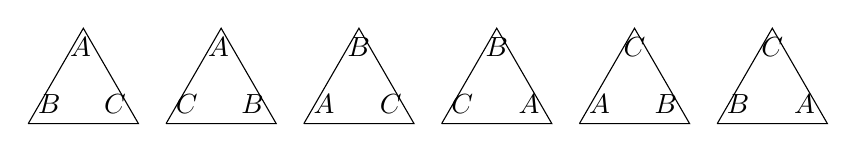
\begin{tikzpicture}[scale=0.7]
          \draw (-1,0)--(1,0)--(0,1.732)--(-1,0);
          \draw (-3.5,0)--(-1.5,0)--(-2.5,1.732)--(-3.5,0);
          \draw (-6,0)--(-4,0)--(-5,1.732)--(-6,0);
          \draw (4,0)--(6,0)--(5,1.732)--(4,0);
          \draw (1.5,0)--(3.5,0)--(2.5,1.732)--(1.5,0);
          \draw (6.5,0)--(8.5,0)--(7.5,1.732)--(6.5,0);
          \node[below] at (-5.05, 1.732) {$A$};
          \node[below] at (-2.55, 1.732) {$A$};
          \node[below] at (-0, 1.732) {$B$};
          \node[below] at (2.5, 1.732) {$B$};
          \node[below] at (5, 1.732) {$C$};
          \node[below] at (7.5, 1.732) {$C$};
          \node[above right] at (-6,0) {$B$};
          \node[above right] at (-3.5,0) {$C$};
          \node[above right] at (-1,0) {$A$};
          \node[above right] at (1.5,0) {$C$};
          \node[above right] at (4,0) {$A$};
          \node[above right] at (6.5,0) {$B$};
          \node[above left] at (-4.05,0) {$C$};
          \node[above left] at (-1.55,0) {$B$};
          \node[above left] at (0.95,0) {$C$};
          \node[above left] at (3.45,0) {$A$};
          \node[above left] at (5.95,0) {$B$};
          \node[above left] at (8.45,0) {$A$};
      \end{tikzpicture}
      \end{center}
      \item Dih$(4)$ is the group of all rotations and reflections that preserve the structure of the regular tetrahedron in $\mathbb{R}^{3}$. An incorrect, yet somewhat useful, way of visualizing this group is to imagine a square in $\mathbb{R}^{2}$. However, the points are not pairwise equidistant and therefore does not preserve symmetry between all points.
      \item Dih$(n)$ is similarly the group of all rotations and reflections that preserve the structure of a regular $(n-1)$-simplex in $\mathbb{R}^{n-1}$. 
    \end{enumerate}
  \end{example} 

  \begin{example}[Klein 4 Group]
    The \textbf{Klein 4-Group} can be described as the symmetry group of a non-square rectangle. With the three non-identity elements being horizontal reflection, vertical reflection, and 180-degree rotation. 

    \begin{figure}[H]
      \centering 
      \begin{tabular}{c|cccc}
        \hline
        $\cdot$ & $e$ & $a$ & $b$ & $c$ \\
        \hline
        $e$ & $e$ & $a$ & $b$ & $c$ \\
        $a$ & $a$ & $e$ & $c$ & $b$ \\
        $b$ & $b$ & $c$ & $e$ & $a$ \\
        $c$ & $c$ & $b$ & $a$ & $e$ \\
        \hline
      \end{tabular}
      \caption{Multiplication table for the Klein 4-group ($V_4$)} 
      \label{fig:klein4group}
    \end{figure}
  \end{example}

  \begin{example}[Groups of Order 4]
    There are only 2 groups of order 4. 
    \begin{figure}[H]
      \centering
      \begin{subfigure}[b]{0.48\textwidth}
        \centering
        \begin{tabular}{|c|c|c|c|c|}
          \hline
          $C_4$ & $e$ & $a$ & $a^2$ & $a^3$ \\
          \hline
          $e$ & $e$ & $a$ & $a^2$ & $a^3$ \\
          \hline
          $a$ & $a$ & $a^2$ & $a^3$ & $e$ \\
          \hline
          $a^2$ & $a^2$ & $a^3$ & $e$ & $a$ \\
          \hline
          $a^3$ & $a^3$ & $e$ & $a$ & $a^2$ \\
          \hline
        \end{tabular}
        \caption{Cyclic group $C_4$}
      \end{subfigure}
      \hfill 
      \begin{subfigure}[b]{0.48\textwidth}
        \centering
        \begin{tabular}{|c|c|c|c|c|}
          \hline
          $V$ & $e$ & $a$ & $b$ & $c$ \\
          \hline
          $e$ & $e$ & $a$ & $b$ & $c$ \\
          \hline
          $a$ & $a$ & $e$ & $c$ & $b$ \\
          \hline
          $b$ & $b$ & $c$ & $e$ & $a$ \\
          \hline
          $c$ & $c$ & $b$ & $a$ & $e$ \\
          \hline
        \end{tabular}
        \caption{Klein four-group $V$}
      \end{subfigure}
      \caption{Cayley tables for the two groups of order 4}
      \label{fig:order4groups}
    \end{figure} 
  \end{example}

\subsubsection{Lie Groups} 

  \begin{definition}[General Linear Group]
    The \textbf{general linear group}, denoted GL$(V)$, is the set of all bijective linear mappings from $V$ to itself. Similarly, GL$_{n}(\mathbb{F})$, or GL $(n, \mathbb{F})$ is the set of all nonsingular $n \times n$ matrices over the field $\mathbb{F}$. Due to the same dimensionality of the following spaces, it is clear that GL$(V) \simeq$ GL$(\mathbb{F}^{n}) \simeq$ GL$_{n}(\mathbb{F})$. The \textbf{special linear group}, denoted SL$_{n} (\mathbb{F})$ or SL$(n, \mathbb{F})$, is the set of $n\times n$ matrices a with determinant $1$. SL$_{n}(\mathbb{F})$ is a subgroup of GL$_{n}(\mathbb{F})$, which is a subset of the ring of all $n \times n$ matrices over field $\mathbb{F}$, denoted $\mathbb{L}_{n}(\mathbb{F})$. 
  \end{definition}

  \begin{definition}[Translation Group]
    The group of all translations in the space $V$ is denoted Tran$\,V$. Its elements are usually denoted as $t_{u}$, where $u$ is the vector that is being translated by. It can also be interpreted as shifting the origin by $-u$. It is clear that Tran$\,V \simeq V$. 
  \end{definition}

  \begin{definition}[General Affine Group]
    The \textbf{general affine group} is the pair of all transformations
    \begin{equation}
      \text{GA} (V) \equiv \text{Tran}(V) \times \text{GL}(V)
    \end{equation}
  \end{definition}

  \begin{definition}[Isometries]
    The \textbf{Euclidean group} of \textbf{isometries} in the Euclidean space $\mathbb{E}^{n}$ (with the Euclidean norm), denoted Isom$\, \mathbb{E}^{n}$ or $\mathbb{E}(n)$, consists of all distance-preserving bijections from $\mathbb{E}^{n}$ to itself, called \textbf{motions} or \textbf{rigid transformations}. It consists of all combinations of rotations, reflections, and translations. The \textbf{special Euclidean group} of all isometries that preserve the \textbf{handedness} of figures is denoted $\mathbb{SE}(n)$, which is comprised of all combinations rotations and translations called \textbf{rigid motions} or \textbf{proper rigid transformations}.
  \end{definition}

  \begin{definition}[Orthogonal Group]
    The \textbf{orthogonal group}, denoted $\O(n)$, consists of all isometries that preserve the origin, i.e. consists of rotations and reflections. The \textbf{special orthogonal group}, denoted SO$(n)$, is a subgroup of O$(n)$ consisting of only rotations. We can see that 
    \begin{equation}
      \text{O}(n)=\frac{\text{Isom}\, \mathbb{E}^{n}}{\text{Tran}\,V}
    \end{equation}
  \end{definition}

  \begin{definition}[Transitive]
    A transformation group $G$ is called \textbf{transitive} if for any $x, y \in X$, there exists a $\phi \in G$ such that $y = \phi(x)$. 
  \end{definition}

  \begin{example}
    Tran$(V)$ and GA$(V)$ are transitive groups. 
  \end{example}

  \begin{definition}[Congruence Classes]
    Let $X$ be a set and $G$ its transformation group on $X$. The way we define $G$ determines the \textbf{geometry} of $X$. More specifically, a figure $F_{1} \subset X$ is \textbf{equivalent} or \textbf{congruent} to $F_{2} \subset X$ iff there exists $\phi \in G$ such that $F_{2} = \phi (F_{1})$ (or equivalently, $F_{1} = \phi (F_{2})$). This is an equivalence relation since
    \begin{enumerate}
      \item $F \sim F$. 
      \item $F \sim H \implies H \sim F$. 
      \item $F \sim H, H \sim K \implies F \sim K$
    \end{enumerate}
    Two figures that are in the same equivalence class are known to be \textbf{congruent} with respect to the geometry of $X$ induced by $G$. 
  \end{definition}

  Clearly, if two figures are congruent in Euclidean geometry, then they are congruent in Affine geometry, since E$(n) \subset$ GA$(n)$. 

\subsection{Subgroups}

  We have seen a few examples of subgroups, but we will heavily elaborate on here. We know that given a set, we can define an equivalence relation on it to get a quotient set. Now if we have a group, defining any such relation may not be compatible with the group structure. Therefore, it would be nice to have some principles in which we can construct such compatible equivalence classes. Fortunately, we can do such a thing by taking a subgroup $H \subset G$ and ``shifting'' it to form the cosets of $G$, which are the equivalence classes. 
  
  \begin{definition}[Coset]
    Given a group $G$, $g \in G$, and subgroup $H$, 
    \begin{enumerate}
      \item A \textbf{left coset} is $g H \coloneqq \{g h \mid h \in H \}$. 
      \item A \textbf{right coset} is $H g \coloneqq \{h g \mid h \in H \}$. 
      \item If $G$ is abelian, then the \textbf{coset} is $gH \coloneqq \{g + h \mid h \in H\}$. 
    \end{enumerate}
    This divides the group into equivalence classes $g \mapsto [g] = gH$, and we write (for left cosets)
    \begin{equation}
      a \equiv b \pmod{H} \iff a = b h \text{ for some } h \in H
    \end{equation}
  \end{definition}
  \begin{proof}
    We show that this indeed forms an equivalence class. 
  \end{proof}

  With this partitioning scheme in mind, the following theorem on the order of such groups becomes very intuitive, and has a lot of consequences. 

  \begin{theorem}[Lagrange's Theorem]
    Let $G$ be a finite group and $H$ its subgroup. Then 
    \begin{equation}
      |G| = [G:H] |H|
    \end{equation}
    where $[G:H]$, called the \textbf{index of $H$}, is the number of cosets in $G$. Therefore, the order of a subgroup of a finite group divides the order of the group. 
  \end{theorem}
  \begin{proof}
    The union of the $[G:H]$ disjoint cosets is all of $G$. On the other hand, every $H$ is in one-to-one correspondence with each coset $aH$, so every coset has $|H|$ elements. Therefore, there are $[G:H] |H|$ elements altogether. 
  \end{proof}

  However, the converse is usually false, as there is a group of order 12 having no subgroup of order 6. 

  \begin{corollary}
    The order of any element of a finite group divides the order of the group. 
  \end{corollary}
  \begin{proof}
    Take any $a \in G$ and construct the cyclic subgroup $\langle a \rangle \subset G$. Then by Lagrange's theorem, $|a| = |\langle a \rangle|$ divides $|G|$. 
  \end{proof}

  \begin{corollary}
    Every finite group of a prime order is cyclic. 
  \end{corollary}
  \begin{proof}
    Let $a \in G$ be any element other than the identity $e$, and consider $\langle a \rangle \subset G$. The order must divide $|G|$ which is prime, so $|a| = 1$ or $|G|$. But $|a| \neq 1$ since we did not choose the identity, so $|a| = |G| \implies \langle a \rangle = G$. 
  \end{proof}

  \begin{corollary}
    If $|G| = n$ and $a \in G$ is arbitrary, then $a^n = e$. 
  \end{corollary}
  \begin{proof}
    Let $|a| = k$. Then $k \mid n$, and so $a^n = a^{kl} = (a^k)^l = e^l = e$. 
  \end{proof}

  \begin{corollary}[Fermant's Little Theorem]
    Let $p$ be a prime number. The multiplicative group $\mathbb{Z}_{p} \setminus \{0\}$ of the field $\mathbb{Z}_{p}$ is an abelian group of order $p-1 \implies g^{p-1} = 1$ for all $g \in \mathbb{Z}_{p} \setminus \{0\}$. So,
    \begin{equation}
      a^{p-1} \equiv 1 \iff a^{p} \equiv a \pmod{p}
    \end{equation}
  \end{corollary} 

  \begin{definition}[Normal Subgroups]
    A subgroup $N \subset G$ is a \textbf{normal subgroup} iff the left cosets equal the right cosets. That is, $\forall b \in G, h \in H$. 
    \begin{equation}
      b^{-1} h b \in H
    \end{equation}
    Every subgroup of an abelian group is normal. 
  \end{definition} 

  The concept of normal subgroups allow us to endow on the quotient set a group structure. 

  \begin{definition}[Quotient Group]
    Given a group $G$ and a normal subgroup $H$, the \textbf{quotient group} $G/H$ is the set of left cosets $aH$ with the operation 
    \begin{equation}
      aH \, bH = abH
    \end{equation}
  \end{definition}

  \begin{lemma} 
    A subgroup $H \subset G$ is normal if and only if there exists a group homomorphism $\phi: G \rightarrow G^\prime$ with $\ker{\phi} = H$. 
  \end{lemma}
  \begin{proof}
    We prove bidirectionally. 
    \begin{enumerate}
      \item $(\rightarrow)$. Since $H$ is normal, we can form the quotient group $G/H$. Let $\phi: G \rightarrow G/H$ be defined $\phi(a) = aH$. Then, 
      \begin{align}
        \ker{\phi} = \phi^{-1}(eH) & = \{a \in G \mid aH = eH = H \} \\
                                   & = \{a \in G \mid a \in H \}
      \end{align}
      Therefore, $\phi$ is a homomorphism because $\phi(ab) = abH = (aH)(bH)$. 
    \end{enumerate}
  \end{proof}

  \begin{theorem}[Quotient Maps are Homomorphisms]
    The map $\pi: G \rightarrow G/H$ is a group homomorphism, and the \textbf{quotient group} is the set of left cosets with 
  \end{theorem}
  \begin{proof}
    
  \end{proof} 

  \begin{corollary}
    If $|G| = n$, then $g^{n} = e$ for all $g \in G$. 
  \end{corollary}

  \begin{definition}[Euler's Totient Function]
    \textbf{Euler's Totient Function}, denoted $\varphi(n)$, consists of all the numbers less than or equal to $n$ that are coprime to $n$. 
  \end{definition}

  \begin{theorem}[Euler's Theorem]
    For any $n$, the order of the group $\mathbb{Z}_{n} \setminus \{0\}$ of invertible elements of the ring $\mathbb{Z}_{n}$ equals $\varphi(n)$, where $\varphi$ is Euler's totient function. In other words with $G = \mathbb{Z}_{n} \setminus \{0\}$, 
    \begin{equation}
      a^{\varphi(n)} \equiv 1 \pmod{n}, \; \text{ where $a$ is coprime to $n$}
    \end{equation}
  \end{theorem}

  \begin{example}
    In $\mathbb{Z}_{125} \setminus \{0\}$, $\varphi(125) = 125 - 25 = 100 \implies 2^{100} \equiv 1 \pmod{125}$
  \end{example}

  \begin{definition}
    Let $G$ be a transformation group on set $X$. Points $x, y \in X$ are equivalent with respect to $G$ if there exists an element $g \in G$ such that $y = g x$. This has already been defined through the equivalence of figures before. This relation splits $X$ into equivalence classes, called \textbf{orbits}. Note that cosets are the equivalence classes of the transformation group $G$; oribits are those of $X$. We denote it as
    \begin{equation}
      Gx \equiv \{ g x \;|\;g \in G \}
    \end{equation}
  \end{definition}

  By definition, transitive transformation groups have only one orbit.

  \begin{definition}
    The subgroup $G_{x} \subset G$, where $G_{x} \equiv \{ g \in G | g x = x\}$ is called the \textbf{stabilizer} of $x$.
  \end{definition}

  \begin{example}
    The orbits of $O(2)$ are concentric circles around the origin, as well as the origin itself. The stabilizer of the point $p \neq 0$ is the identity and the reflection across the line $??$. The stabilizer of $0$ is the entire $O(2)$.
  \end{example}

  \begin{example}
    The group $S_n$ is transitive on the set $\{1, 2, ..., n\}$. The stabilizer of $k, (1 \leq k \leq n)$ is the subgroup $H_{k} \simeq S_{n-1}$, where $H_k$ is the permutation group that does not move $k$ at all. 
  \end{example}

  \begin{theorem}
    There exists a 1-to-1 injective correspondence between an orbit $G_x$ and the set $G / G_{x}$ of cosets, which maps a point $y = g x \in G x $ to the coset $g G_x$. 
  \end{theorem}

  \begin{definition}
    The \textbf{length of an orbit} is the number of elements in it. 
  \end{definition}

  \begin{corollary}
    If $G$ is a finite group, then 
    \begin{equation}
      |G| = |G_x| |G x|
    \end{equation}
    In fact, there exists a precise relation between the stabilizers of points of the same orbit, regardless of $G$ being finite or infinite: 
    \begin{equation}
      G_{g x} = g G_{x} g^{-1}
    \end{equation}
  \end{corollary}

\subsection{Products and Extensions of Groups} 

\subsubsection{Direct Products}

  \begin{definition}[Direct Product]
    The \textbf{direct product} of two groups $G$ and $H$ is denoted
    \begin{equation}
      G \times H \equiv \{ (g, h)\;|\; g \in G, h \in H \}
    \end{equation}
    Note that the product need not be binary (nor must it be of finite arity). 
  \end{definition}

  \begin{example}
    The \textbf{general affine group} is defined 
    \begin{equation}
      \text{GA}(V) \equiv \text{Tran}\,V \times \text{GL}(V)
    \end{equation}
  \end{example}

  \begin{example}
    The \textbf{Galileo Group} is the transformation group of spacetime symmetries that are used to transform between two reference frames which differ only by constant relative motion within the constructs of Newtonian physics. It is denoted 
    \begin{equation}
      \text{Tran}\;\mathbb{R}^{4} \times H \times \text{O} (3)
    \end{equation}
    where $H$ is the group of transformations of the form 
    \begin{equation}
      (x, y, z, t) \longmapsto (x+at, y+bt, z+ct, t)
    \end{equation}
  \end{example}

  \begin{example}
    The \textbf{Poincaré Group} is the symmetry group of spacetime within the principles of relativistic mechanics, denoted
    \begin{equation}
      G = \text{Tran}\; \mathbb{R}^{4} \times \text{O}_{3,1}
    \end{equation}
    where O$_{3,1}$ is the group of linear transformations preserving the polynomial 
    \begin{equation}
      x^{2} + y^{2} + z^{2} - t^{2}
    \end{equation}
  \end{example} 

\subsubsection{Semidirect Products} 

\subsubsection{Group Extensions}

\subsection{Group Actions}

  \begin{definition}[Group Action]
    Let $G$ be a group, $X$ a set. Then, a (left) group action of $G$ on $X$ is a function: 
    \begin{equation}
      \varphi: G \times X \longrightarrow X, \; (g,x) \longmapsto \varphi(g,x)
    \end{equation}
    satisfying two axioms:
    \begin{enumerate}
      \item Identity. $\forall x \in X, \varphi(e, x) = x$. 
      \item Compatibility. $\forall g, h \in G \text{ and } \forall x \in X, \varphi(gh, x) = \varphi(g, \varphi(h, x))$.
    \end{enumerate}
    The group $G$ is said to \textbf{act on} $X$. $X$ is called a \textbf{G-set}. The two axioms, furthermore, imply that for every $g \in G$, the function that maps $x \in X$ to $ \varphi(g, x) \in X$ is a bijective map, since the inverse is the function mapping $x \mapsto \varphi(g^{-1}, x)$. \\
    $(g, x)$ can be interpreted as the element $g$ in the transformation group $G$ acting on an element $x$ in $X$.
  \end{definition}

  \begin{example}
    Isom$\,\mathbb{R}^{3}$ acts on $\mathbb{R}^{3}$ since every element $g \in$ Isom$\,\mathbb{R}^{3}$ acts on the entire space $\mathbb{R}^{3}$. 
  \end{example}

  \begin{example}
    $S_n$ acts on $\{1, 2, ..., n\}$by permuting its elements.
  \end{example}

  \begin{example}
    The GA$(V)$ acts transitively on the points of an affine space.
  \end{example}

  \textbf{Equivalent Interpretation of Group Actions}
  Note that this group action $G$ on space $X$ identifies a group homomorphism into the group of automorphisms of that space. Given an abstract group element $g \in G$, $\varphi(g, \cdot): X \longrightarrow X$ is defined accordingly, where $\varphi(g, \cdot) \in $ Aut$(X)$. So alternatively, we can interpret a group action as a homomorphism from $G$ to Aut$(X)$. 
  \begin{equation}
    \phi: G \longrightarrow \text{Aut}(X), \; g \mapsto \phi(g) = \varphi(g,\cdot)
  \end{equation}

  \begin{definition}[Representation]
    A group action on a finite-dimensional vector space $X$ is called a \textbf{representation} of that group. 
  \end{definition}

\subsection{Abelian Groups}

  First, note that the successive addition of elements of an additive abelian group can be represented by integer multiplication. 
  \begin{equation}
    x + x + ... + x = n x, \; n \in \mathbb{Z}
  \end{equation}
  Similarly, we can take the integer power of an element to represent successive multiplication in a multiplicative abelian group. 

  \begin{lemma}
    It is easy to check that in an additive abelian group $A$, with $a, b \in A$ and $k, l \in \mathbb{Z}$, 
    \begin{align}
      & k (a + b) = k a + k b \\
      & (k + l) a = k a + l a \\
      & (k l) a = k (l a)
    \end{align}
    which implies
    \begin{equation}
      k(a - b) = k a - k b, \; (k - l) a = k a - l a
    \end{equation}
  \end{lemma}

  \begin{definition}
    For any subset $S \subset A$, the collection of all linear combinations 
    \begin{equation}
      k_1 a_1 + k_2 a_2 + ... + k_n a_n, \; k_i \in \mathbb{Z}, a_i \in S
    \end{equation}
    is the smallest subgroup of $A$ containing $S$, called the \textbf{subgroup generated by $S$} and denoted $\langle S \rangle$. If $\langle S \rangle = A$, then we say that $A$ is \textbf{generated} by $S$, or that $S$ is a \textbf{generating set} of $A$. 
  \end{definition}

  \begin{definition}
    An abelian group that has a finite generating set is called \textbf{finitely generated}. Finitely generated abelian groups are similar to finite dimensional vector spaces. 
  \end{definition}

  \begin{definition}
    A system $\{ a_1, a_2, ..., a_n\}$ of elements of a group $A$ is called \textbf{linearly independent} if $k_1 a_1 + k_2 a_2 + ... + k_n a_n = 0 \implies k_1, k_2, ..., k_n = 0$. A system of linear independent elements that generates $A$ is called a \textbf{basis}. 
  \end{definition}

  Note that every finite dimensional vector has a basis, but not every finitely generated abelian group has one. For example, $(\mathbb{Z}_n, +)$ is generated by one element, but it has no basis since every element $a \in \mathbb{Z}_n$ satisfies the nontrivial relation $n a = 0$. 

  \begin{definition}
    A finitely generated abelian group is \textbf{free} if it has a basis. 
  \end{definition}

  \begin{theorem}
    All bases of a free abelian group $L$ contain the same number of elements. 
  \end{theorem}

  \begin{definition}
    The \textbf{rank} of a free abelian group $L$ is the number of elements in its basis. It is denoted rk$L$. The zero group is regarded as a free abelian group of rank $0$. 
  \end{definition}

  \begin{theorem}
    Every free abelian group $L$ of rank $n$ is isomorphic to the group $\mathbb{Z}^n$ of integer rows of length $n$. 
  \end{theorem}

  \begin{theorem}
    Every subgroup $n$ of a free abelian group $l$ of rank $n$ is a free abelian group of rank $ \leq n$. 
  \end{theorem}

  Note that unlike a vector space, a free abelian group of positive rank contains subgroups of the same rank that do not conside with the whole group. For example, the subgroup $m \mathbb{Z} \subset \mathbb{Z}, m > 0$ has rank $1$, just as the whole group. 

  Moreover, a free abelian group of rank $n$ can be embedded as a subgroup into an $n$-dimensional Euclidean vector space $E^n$. To do this, let $\{e_1, e_2, ..., e_n\}$ be a basis of $E^n$. Then, the subgroup generated by these basis vectors is the set of vectors with integer components, which is a free abelian group of rank $n$. This subgroup obtained as such is called a \textbf{lattice} in $E^n$. 

  \begin{definition}
    A subgroup $L \subset E^n$ is \textbf{discrete} if every bounded subset of $E^n$ contains a finite number of elements in $L$. Clearly, every lattice is discrete, and a subgroup generated by a linearly independent system of vectors (i.e. a lattice in a subspace of $E^n$) is discrete. 
  \end{definition}

  \begin{lemma}
    A subgroup $L \subset E^n$ is discrete if and only if its intersection with any neighborhood of $0$ consists of $0$ itself. 
  \end{lemma}

  \begin{theorem}
    Every discrete subgroup $L \subset E^n$ is generated by a linearly independent system of vectors of $E^n$. 
  \end{theorem}

  \begin{corollary}
    A discrete subgroup $L \subset E^n$ whose linear span coincides with $E^n$ is a lattice in $E^n$. 
  \end{corollary}

  Lattices in $E^3$ play an important role in crystallography since the defining feature of a crystal structure is the periodic repetition of the configuration of atoms in all three dimensions. More explicitly, let $\Gamma$ be the symmetry group of the crystal structure and let $\mathcal{L}$ be the group of all vectors $a$ such that the parallel translation $t_a \in \Gamma$. Then, $\mathcal{L}$ is a discrete subgroup of $E^n$ and thus, is a lattice in $E^3$. More specifically, we can present 
  \begin{equation}
    \Gamma \equiv \text{Dih}\,C \times \mathcal{L}
  \end{equation}
  where Dih$\, C$ is the Dihedral group of the crystal structure that preserves its lattices. 

  \begin{definition}
    An \textbf{integral elementary row transformation} of a matrix is a transformation of one of the following three types: 
    \begin{enumerate}
      \item adding a row multiplied by an integer to another row
      \item interchanging two rows
      \item multiplying a row by $-1$ 
    \end{enumerate}
    An \textbf{integral elementary column transformation} is defined similarly. 
  \end{definition}

  \begin{lemma}
    Every integral rectangular matrix $C = (c_{i j})$ can be reduced by integral elementary row transformations to the diagonal matrix diag$(u_1, ..., u_p)$, where $u_1, u_2, ..., u_p \geq 0$ and $u_i | u_{i+1}$ for $i = 1, 2, ..., p -1$. 
  \end{lemma}

  \begin{example}
    The following matrix can be reduced (with a few steps now shown) to the stated form. 
    \begin{equation}
    \begin{pmatrix} 2&6&2 \\ 2&3&4 \\ 4&2&4 \end{pmatrix} \rightarrow 
    \begin{pmatrix} 2&3&4 \\ 0&-3&2 \\ 4&2&4 \end{pmatrix} \rightarrow
    \begin{pmatrix} 1&0&0 \\ 0&6&14 \\ 0&8&12 \end{pmatrix} \rightarrow
    \begin{pmatrix} 1&0&0 \\ 0&2&0 \\ 0&0&20\end{pmatrix}
    \end{equation}
    where $1|2$ and $2|20$. 
  \end{example}

  Note that for $n \times 1$ or $1 \times n$ matrices, this procedure is precisely the Euclidean algorithm that produces the GCD of $n$ integers. 

  \begin{lemma}
    Given square integral matrix $C$ with  reduced form diag$(u_1, ..., u_p)$, 
    \begin{equation}
      u_i = \frac{d_i}{d_{i-1}}
    \end{equation}
    where $d_i$ is the GCD of the minors of order $i$ of the original matrix $C$. Recall that a minor of a matrix is the determinant of the matrix with one of its rows and columns removed. $d_0$ is assumed to equal $1$. This implies that the numbers $u_1, u_2, ..., u_p$, along with the reduced form, are uniquely determined by $C$. 
  \end{lemma}

  \begin{theorem}
    For any subgroup $N$ of a free abelian group $L$ of rank $n$, there exists a basis $\{e_1, ..., e_n\}$ of $L$ and natural numbers $u_1, ..., u_m, \; (m \leq n)$, such that $\{u_1 e_1, ..., u_m e_m\}$ is a basis fo the group $N$ and $u_i | u_{i+1}$ for $i = 1, 2, ..., m-1$. 
  \end{theorem}
    

\section{Rings} 

  We have extensively talked about groups, and now we look at an algebraic structure called a ring that has two operations. As we introduce rings, we will use the integers as the primary structure to demonstrate our theorems, along with the ring of continuous functions and the ring of matrices. 

  \begin{definition}[Ring]
    A \textbf{ring} is a set $(R, +, \times)$ equipped with two operations, called addition and multiplication. It has properties: 
    \begin{enumerate}
      \item $R$ is an abelian group with respect to $+$, where we denote the additive identity as $0$ and the additive inverse of $x$ as $-x$. 
      \item $R$ is a monoid with respect to $\times$, where we denote the multiplicative identity as $1$, also known as the \textbf{unity}. 
      \item $\times$ is both left and right distributive with respect to addition $+$
      \begin{align}
        a \times (b + c) & = a\times b + a\times c \\ 
        (a + b) \times c & = a\times c + b\times c 
      \end{align}
      for all $a, b, c \in \mathbb{R}$. 
    \end{enumerate} 
    If $\times$ is commutative, $R$ is called a \textbf{commutative ring}. 
  \end{definition}

  In fact, in some cases associativity (in multiplication) or the existence of the multiplicative identity is not even assumed, though we will do it here.\footnote{If a multiplicative identity is not assumed, then this is called an \textit{rng}, or a \textit{rung}.} It turns out that the existence of a multiplicative inverse, also called a \textit{unity}, forces addition to be abelian. Try computing the product $(1 + 1)(a + b)$ in two different ways. 
  \begin{align}
    (1 + 1)(a + b) & = 1(a + b) + 1(a + b) = a + b + a + b \\
    (1 + 1)(a + b) & = (1 + 1)a + (1 + 1)b = a + a + b + b
  \end{align}
  and so from the group properties, we necessarily have $b + a = a + b$. 

  \begin{figure}[H]
    \centering 
    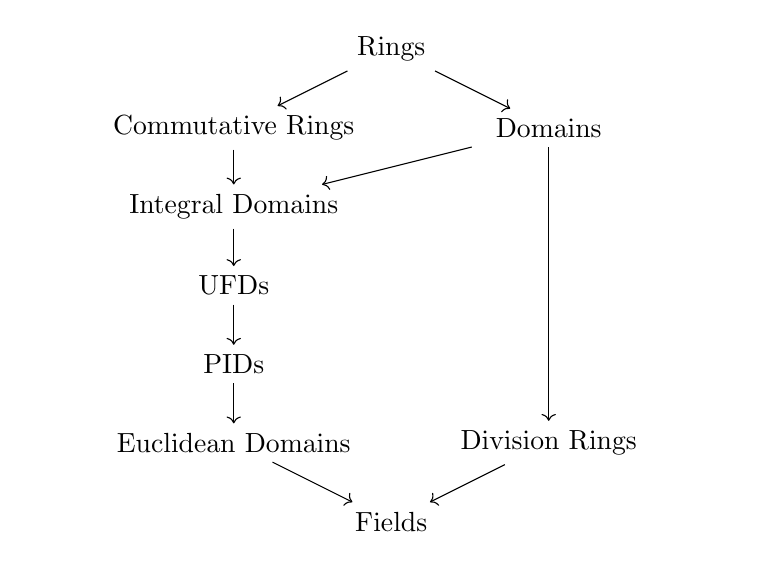
\begin{tikzpicture}[
      node distance=2cm,
      box/.style={
          text width=5cm,
          align=center
      }
      ]
      % Nodes for ring types
      \node[box] (rings) at (0,0) {Rings};
      \node[box] (comm) at (-2,-1) {Commutative Rings};
      \node[box] (domains) at (2,-1) {Domains};
      \node[box] (int) at (-2,-2) {Integral Domains};
      \node[box] (ufd) at (-2,-3) {UFDs}; % Added UFD between ID and PID
      \node[box] (divring) at (2,-5) {Division Rings};
      \node[box] (pid) at (-2,-4) {PIDs}; % Moved PID down
      \node[box] (euc) at (-2,-5) {Euclidean Domains}; % Moved ED down
      \node[box] (fields) at (0,-6) {Fields}; % Moved Fields down
      
      % Left path arrows
      \draw[->] (rings) -- (comm);
      \draw[->] (comm) -- (int);
      \draw[->] (int) -- (ufd); % New arrow to UFD
      \draw[->] (ufd) -- (pid); % New arrow from UFD to PID
      \draw[->] (pid) -- (euc);
      \draw[->] (euc) -- (fields);
      \draw[->] (divring) -- (fields);
      
      % Right path arrows
      \draw[->] (rings) -- (domains);
      \draw[->] (domains) -- (int);
      \draw[->] (domains) -- (divring);
    \end{tikzpicture}
    \caption{Basic hierarchy of rings with UFDs included.} 
    \label{fig:ring_hierarchy}
  \end{figure}

  Since a ring is a group with respect to addition, we know from \ref{thm:unique_add_inverse} that additive inverses are unique. However, we can say a little more with rings because of the distributive property. 

  \begin{lemma}[Additive Inverses] 
    Let $R$ be a ring. Then, for all $a, b \in R$, 
    \begin{enumerate}
      \item $0a = a0 = 0$. 
      \item $(-a)b = a(-b) = -(ab)$. 
      \item $(-a)(-b) = ab$. 
      \item The identity $1$ is unique and $-a = (-1)a$. 
    \end{enumerate}
  \end{lemma}
  \begin{proof}
    We can see that 
    \begin{align}
      -1 + 1 = 0 & \implies (-1 + 1) \times a = 0 \times a \\
    \end{align}
    and therefore by definition $-1 \times a$ must be the additive inverse. 
  \end{proof} 

  We will provide some examples of rings, though we have not properly defined some of them yet. We have only properly defined the power set ring and the integer ring in set theory. As for the rest, I hope the reader is familiar enough with these materials to at least recognize that they are rings. 

  \begin{example}[Power Set]
    Given a set $X$, $(2^X, \bigtriangleup, \cap)$ is a commutative associative ring with respect to the operations of symmetric difference $M \bigtriangleup N \coloneqq (M \setminus N) \cup (N \setminus M)$ and intersection. The additive identity is $\emptyset$ and the multiplicative identity is $X$. We can clearly see that both operations are commutative and $\cap$ is associative. 
    \begin{align*}
      M \bigtriangleup N & = (M \setminus N) \cup (N \setminus M) \equiv N \bigtriangleup M \\
      M \cap N & = N \cap M \\
      M \cap N \cap P & = (M \cap N) \cap P = M \cap (N \cap P)
    \end{align*}
  \end{example}

  \begin{example}[Number Systems]
    $(\mathbb{Z}, +, \times)$, $(\mathbb{Q}, +, \times)$, $(\mathbb{R}, +, \times)$, $(\mathbb{C}, +, \times)$ are all commutative rings, with additive and multiplicative identities $0$ and $1$. 
  \end{example}

  \begin{example}[Matrix Rings]
    The set of matrices $\mathbb{R}^{n \times n}$\footnote{really over any field and even more generally a ring $R$} forms a noncommutative ring under matrix addition $+$ and multiplication $\times$. It has the additive and multiplicative identities $0$ and $I_{n}$. This forms a non-commutative ring for $n > 1$, even when $R$ is commutative.
  \end{example}

  \begin{example}[Polynomials]
    The set of all polynomials over the reals are a ring. 
  \end{example}

  \begin{example}[Continuous Functions]
    The set of all continuous functions $f: \mathbb{R} \rightarrow \mathbb{R}$ is a ring under point-wise addition and multiplication. 
  \end{example}

  Next, just like how we did for groups, we can talk about subrings. 

  \begin{definition}[Subring]
    Given ring $(R, +, \times)$ a \textbf{subring} $(S, +, \times)$ is a ring such that $S \subset R$. $S$ is called a \textbf{proper subring} if $S \subsetneq R$. 
  \end{definition}

  \begin{example}[Quadratic Field]
    Let $D \in \mathbb{Q}$ be a square-free rational number (as in $D$ cannot be expressed as the perfect square of another rational). Now let us consider the set 
    \begin{equation}
      \mathbb{Q} (\sqrt{D}) \coloneqq \{a + b \sqrt{D} \mid a, b \in \mathbb{Q} \}
    \end{equation}
    equipped with component-wise addition and multiplication where $\sqrt{D}^2 = D$ and the rational commute with $\sqrt{D}$. This is indeed a commutative subring of $\mathbb{R}$. 
  \end{example}

  \begin{example}[Gaussian Integers]
    The \textbf{Gaussian integers} is the set 
    \begin{equation}
      \mathbb{Z}[i] \coloneqq \{a + bi \mid a, b \in \mathbb{Z} \} \subset \mathbb{C}
    \end{equation}
    equipped with component-wise addition and multiplication where $i^2 = 1$ and reals commute with $i$. This is indeed a commutative subring of $\mathbb{C}$. 
  \end{example}

  \begin{theorem}[Intersections of Subrings is a Subring]
    If $S_1, S_2$ are subrings of $R$, then $S_1 \cap S_2$ is a subring. 
  \end{theorem}

  Finally, we will mention a product ring. 

  \begin{definition}[Direct Product of Rings]
    Given rings $(R, +_R, \times_R)$ and $(S, +_S, \times_S)$, the direct product of the rings is the set $R \times S$ with the operations 
    \begin{enumerate}
      \item $(r_1, s_1) + (r_2, s_2) \coloneqq (r_1 +_R r_2, s_1 +_S s_2)$. 
      \item $(r_1, s_1) \times (r_2, s_2) \coloneqq (r_1 \times_R r_2, s_1 \times_S s_2)$. 
    \end{enumerate}
  \end{definition}
  \begin{proof}
    The proof is standard. 
  \end{proof}

\subsection{Ring Homomorphisms}

  So far, we have talked about many properties of rings but have not thoroughly gone over their classification. This is what we will do in this section, just like how we have classified groups. It turns out that classifying rings is significantly harder to do so, so we will talk about some low-order finite rings and provide some examples of isomorphisms between more complex rings. 

  \begin{definition}[Ring Homomorphism, Isomorphism]
    A \textbf{ring homomorphism} $f: R \rightarrow S$ is a function that satisfies for all $a, b \in R$
    \begin{enumerate}
      \item $f(a + b) = f(a) + f(b)$
      \item $f(ab) = f(a) f(b)$ 
      \item $f(1_R) = 1_S$\footnote{The reason we need this third is that while $f$ is a group homomorphism with respect to $+$, it automatically follows that $f(0) = 0$. However $f$ is only a monoid homomorphism w.r.t. $\times$, and so we need this extra constraint. }
    \end{enumerate}
    for all $a, b \in R$.\footnote{Note that the first is equivalent to it being a group homomorphism between $(R, +)$ and $(S, +)$. The second property may look like it is a group homomorphism between $(R, \times)$ and $(S, \times)$, but remember that neither are groups and it just states that closure distributes. Combined with the fact that the multiplicative identity matches, $f$ is really a homomorphism of \textit{monoids}. } Furthermore, 
    \begin{enumerate}
      \item A \textbf{ring isomorphism} is a bijective ring homomorphism, and we call rings $R$ and $S$ isomorphic, denoted $R \simeq S$ if there exists an isomorphism between them. 
      \item A \textbf{ring endomorphism} is a ring homomorphism onto itself. 
      \item A \textbf{ring automorphism} is an isomorphism from a ring to itself. 
    \end{enumerate}
  \end{definition} 

  \begin{example}[Homomorphisms of Rings]
    We provide some simple examples of ring homomorphisms. 
    \begin{enumerate}
      \item The identity map $\iota : R \to R$ is a ring automorphism. 
      \item If $R \subset S$ as rings, then the canonical injection map $\iota: R \to S$ is a ring homomorphism. 
      \item Complex conjugation $z \in \mathbb{C} \mapsto \bar{z} \in \mathbb{C}$ is a ring automorphism. 
      \item Differentiation is a ring automorphism over the polynomial ring $\mathbb{R}[x]$. 
    \end{enumerate}
  \end{example} 

  \begin{definition}[Kernel]
    The \textbf{kernel} of a ring homomorphism $f: R \rightarrow S$ is the preimage of $0 \in S$.\footnote{Note that this is the additive identity, not the multiplicative identity. We must specify which identity, unlike a group which has just one identity.}
  \end{definition}

  \begin{lemma}[Images and Kernels of Ring Homomorphisms]
    If $f: R \rightarrow S$ is a ring homomorphism, then 
    \begin{enumerate}
      \item $\im{f}$ is a subring of $S$. 
      \item $f$ is injective iff $\ker{f} = \{0\}$. 
    \end{enumerate}
  \end{lemma}
  \begin{proof}
    For the first claim, let $x, y, z \in \im{f}$. Then $x = f(a), y = f(b), z = f(c)$ for some $a, b \in R$. 
    \begin{enumerate}
      \item \textit{Closed under Addition}. $x + y = f(a) + f(b) = f(a + b) \in \im{f}$. 
      \item \textit{Associative under Addition}. $(x + y) + z = f(a + b) + f(c) = f((a + b) + c) = f(a + (b + c)) = f(a) + f(b + c) = x + (y + z)$
      \item \textit{Additive Identity}. $f(0) = 0$
      \item \textit{Additive Inverses}. We claim that $x^{-1} = f(a)^{-1} = f(a^{-1})$. Indeed, we have $f(a) f(a^{-1}) = f(a a^{-1}) = f(1) = 1$. 
      \item \textit{Closed under Multiplication}. $xy = f(a) f(b) = f(ab) \in \im{f}$. 
      \item \textit{Multiplicative Identity}. $f(1) = 1$. 
    \end{enumerate}
    For the second claim, we prove bidirectionally. 
    \begin{enumerate}
      \item $(\rightarrow)$. Let $\ker{f} \neq \{0\}$ and call its nonzero element $k$. Then, $f(a + k) = f(a) + f(k) = f(a) + 0 = f(a)$, and so $f(a) = f(a + k)$, which means $f$ is not injective. 
      \item $(\leftarrow)$. Assume that $f$ is not injective. Then there exists $a, b \in R$ s.t. $f(a) = f(b)$. This means that $0 = f(a) - f(b) = f(a - b)$, and so $a - b \in \ker{f}$. 
    \end{enumerate}
  \end{proof}

  Note that $\ker{f}$ is \textit{not} a subring, and we can quickly verify this by noticing that the identity element does not necessarily have to be in the kernel. However, we will see later that this is a specific instance of a more general structure called an \textit{ideal}. 

  \begin{theorem}[Compositions of Ring Homomorphisms]
    Compositions of ring homomorphisms are ring homomorphisms. 
  \end{theorem} 
  \begin{proof}
    Let $R \xrightarrow{f} S \xrightarrow{g} T$ be two ring homomorphisms. We can see that 
    \begin{enumerate}
      \item $(g \circ f)(a + b) = g( f(a) + f(b)) = g(f(a)) + g(f(b))$. 
      \item $g(f(ab)) = g(f(a) f(b)) = g(f(a)) + g(f(b))$ 
      \item $g(f(1_R)) = g(1_S) = 1_T$
    \end{enumerate}
  \end{proof}

  Now let's focus a bit more on ring isomorphisms. The following should be intuitive. 

  \begin{lemma}[Inverse of Ring Isomorphism is an Isomorphism]
    If $f: R \to S$ is a ring isomorphism, then $f^{-1}$ is a ring isomorphism. 
  \end{lemma} 
  \begin{proof}
    Since $f$ is a bijection, $f^{-1}$ is well defined and is a bijection. Now let $x, y \in S$, which implies that $x = f(a), y = f(b)$ for a unique $a, b \in R$. Now we see that $f^{-1}$ satisfies the 3 properties of a ring homomorphism. 
    \begin{enumerate}
      \item $f^{-1} (x + y) = f^{-1} (f(a) + f(b)) = f^{-1}(f(a + b)) = a + b = f^{-1}(a) + f^{-1} (b)$. 
      \item $f^{-1} (x y) = f^{-1} (f(a) f(b)) = f^{-1}(f(a b)) = a b = f^{-1}(a) f^{-1} (b)$. 
      \item $f^{-1}(1_S) = 1_R$. 
    \end{enumerate}
    Therefore, as a bijective ring homomorphism $f^{-1}$ is also a ring isomorphism. 
  \end{proof}

\subsection{Characteristics}

  Note that given a ring $R$, we can pay attention to the subring $\langle 1 \rangle$. This must either be isomorphic to $\mathbb{Z}$ or $\mathbb{Z}_n$, so we can think of it being embedded in $R$. 
  
  \begin{theorem}[Integer Ring Exists in Any Ring]
    For every ring $R$, there exists a unique ring homomorphism $f: \mathbb{Z} \to R$. 
  \end{theorem}
  \begin{proof}
    We know that $f(1_{\mathbb{Z}}) = 1_R$, and so for $n > 0$, 
    \begin{align}
      f(n_{\mathbb{Z}}) & = f(1_{\mathbb{Z}} + \ldots + 1_{\mathbb{Z}}) \\
                        & = f(1_{\mathbb{Z}}) + \ldots + f(1_{\mathbb{Z}}) \\
                        & = 1_R + \ldots + 1_R \\
                        & = n_R
    \end{align} 
    Similarly, we have 
    \begin{align}
      f(-n_{\mathbb{Z}}) & = f(-1_{\mathbb{Z}} - \ldots - 1_{\mathbb{Z}}) \\
                         & = f(1_{\mathbb{Z}}) - \ldots - f(1_{\mathbb{Z}}) \\
                         & = -1_R - \ldots - 1_R \\
                         & = -n_R
    \end{align} 
    Since $\mathbb{Z}$ is a PID, $\ker{f}$---which is an ideal---must be principal, and so $\ker{f} = \langle m \rangle$ for some $m \in \mathbb{Z}$. 
  \end{proof} 

  Therefore, this motivates the following attribute of a ring, i.e. the smallest $\langle m \rangle$ that embeds (an injective homomorphism) into the ring. 

  \begin{definition}[Characteristic Number]
    The \textbf{characteristic} of ring $R$, denoted $\Char(R)$, is defined equivalently. 
    \begin{enumerate}
      \item It is the smallest number of times one must successively add the multiplicative identity $1$ to get the additive identity $0$. 
      \begin{equation}
        1 + 1 + ... + 1 = 0 
      \end{equation}
      If no such number $n$ exists, then $\Char(R) = 0$. 

    \item It is equal to $m$, where $\ker{f} = \langle m \rangle$ for the homomorphism defined above.\footnote{Note that $m$ always exists since $\mathbb{Z}$ is a PID.}
    \end{enumerate}
  \end{definition}

  Often, it is not obvious whether two given rings $R$ and $S$ are isomorphic. The characteristic number is preserved across ring isomorphisms and therefore is a good sanity check. 

  \begin{theorem}[Preservation of Characteristic Number in a Ring Homomorphism]
    $R \simeq S \implies \Char(R) = \Char(S)$. 
  \end{theorem}
  \begin{proof}

  \end{proof}

  However, the converse is not true! If so, we would have completely classified all rings just based on their characteristic number, and the study of rings would end pretty soon. 

  \begin{example}[Same Characteristic does not Imply Isomorphic]
    There exists no isomorphism from $\mathbb{Z}$ to $\mathbb{R}$. 
  \end{example}

  \begin{theorem}[Wilson's Theorem]
    Let $p \in \mathbb{N}$ be prime. Then 
    \begin{equation}
      (p-1)! \equiv -1 \pmod{p}
    \end{equation}
  \end{theorem}
  
  The following corollary isn't really worth stating in my opinion, but it has a popular name that might get mentioned a few times. 

  \begin{corollary}[Freshman's Dream]
    Given a ring $R$ of characteristic $p$, 
    \begin{equation}
      (a + b)^p = a^p + b^p
    \end{equation}
  \end{corollary}
  \begin{proof}
    We have 
    \begin{equation}
      (a + b)^p = \sum_{k = 0}^p \binom{p}{k} a^{p-k} b^{k}
    \end{equation}
    It is clear that 
    \begin{equation}
      \binom{p}{k} = \frac{p (p-1) ... (p - k+1)}{k!}
    \end{equation}
    is divisible by $p$ for all $k \neq 0, p$, so all the middle terms must cancel out to $0$. 
  \end{proof}

\subsection{Divisors and Reducibility} 

  Note that we do not assume that there exists multiplicative inverses in a ring. However, there may be some elements for which multiplicative inverses do exist, i.e. $a, b \in R$ where $ab = 1$. 

  \begin{definition}[Unit]
    A \textbf{unit} of a ring $R$ is an element $u \in R$ that has a multiplicative inverse in $R$. That is, there exists a $v \in R$ s.t. $uv = vu = 1$. 
  \end{definition}

  \begin{example}[Units and Non-Units]
    A ring $R$ may have either none (except for $0$ and $1$), some, or all of its elements as units. 
    \begin{enumerate}
      \item $\mathbb{Z}$ has no non-unity element that is a unit. For example, given $z \in \mathbb{Z}$, there is no element of the form $1/z$.  
      \item In $\mathbb{Q}$, every nonzero element is a unit. Given any element of form $\frac{p}{q} \in \mathbb{Q}$, the element $\frac{q}{p}$ is the multiplicative inverse. 
      \item In $\mathbb{Z}_8$, the units are $1, 3, 5, 7$ as $1 \cdot 1 = 3 \cdot 3 = 5 \cdot 5 = 7 \cdot 7 = 1$. However, $0, 2, 4, 6$ are not units since you can look in $\mod{2}$. 
    \end{enumerate}
  \end{example}

  Another property that we would desire is some sort of decomposition of ring elements as other ring elements. More specifically, the existence of elements $a, b$ such that $ab = 0$ will be of particular interest to us. 

  \begin{definition}[Left, Right Divisor]
    Let $a, b, r \in R$ a ring. 
    \begin{enumerate}
      \item If $ab = r$, then $a$ is said to be a \textbf{left divisor} of $r$ and $b$ a \textbf{right divisor} of $r$. 

      \item $a$ is said to be a left divisor of $r$ if it is a left divisor and a right divisor of $r$: $ax = ya = r$, but $x$ does not necessarily equal $y$. 

      \item If $ab = 0$, then $a$ and $b$ are said to be a \textbf{left zero divisor} and \textbf{right zero divisor}, respectively. 
    \end{enumerate}
    If $R$ is commutative, then we just call $a$ a \textbf{divisor} of $r$ or a \textbf{zero divisor}.\footnote{$a$ is a right divisor of $b \iff \exists x (xa = b) \iff \exists x (ax = b) \iff a$ is a left divisor. } 
  \end{definition}

  \begin{definition}[Reducibility of Elements]
    Let $R$ be a commutative ring and $r \in R$ be nonzero and not a unit. 
    \begin{enumerate}
      \item Then $r$ is \textbf{irreducible} in $R$ if whenever $r = ab$ with $a, b \in R$, at least one of $a, b$ is a unit in $R$. 
      \item Otherwise, $r$ is said to be \textbf{reducible}, and $a, b$ are said to be \textbf{factors}
    \end{enumerate}
  \end{definition}
  
  Note that reducibility is slightly different than the existence of divisors of an element. $r$ may have divisors, but they could also be units. Therefore, irreducibility is weaker than having no divisors. This should not be mixed up with prime/composite elements either, which we have not defined 

  \begin{lemma}[Units and Zero Divisors are Mutually Exclusive]
    An element $a \in R$ can never be both a unit and a zero divisor. 
  \end{lemma}
  \begin{proof}
    Let $a \in R$ be a unit. Then $1 = ab$ for some $b \in R$. Now if $a$ was a zero divisor, then $ra = 0$ for some $r \in R$. However, we have $r(ab) = r1 = r \neq 0 = 0b = (ra)b$, which contradicts associativity. 
  \end{proof}

  Let's go through some examples to see that we can have widely differing behavior in terms of divisors. 

  \begin{example}[Left Divisor But Not Right Divisor in Matrix Ring]
    Let us define the ring
    \begin{equation}
      R = \begin{pmatrix} \mathbb{Z} & \mathbb{Z}_2 \\ 0 & \mathbb{Z} \end{pmatrix} = \bigg\{ \begin{pmatrix} x & y \\ & z \end{pmatrix} \; \bigg| \; x, z \in \mathbb{Z}, y \in \mathbb{Z}_2 \bigg\} 
    \end{equation}
    This should be checked that it is a ring. Let 
    \begin{equation}
      a = \begin{pmatrix} 2 & 0 \\ 0 & 1 \end{pmatrix}, \; b = \begin{pmatrix} 0 & 1 \\ 0 & 0 \end{pmatrix}
    \end{equation}
    Then, we can see that $ab = 0$ but $ba \neq 0$. That is, $b$ is a right zero divisor of $a$, but $b$ is not a left zero divisor. 
  \end{example}

  Note that $0$ is divisible by every element since $0a = 0$ for all $a \in R$. Furthermore, if $p$ was a unit, then it can always be multiplied by $p^{-1}$ and then by any $a \in R$ to get the factorization $a = (a p^{-1}) p$. So $p$ as a unit would divide \textit{every} element in $R$. 

  \begin{example}[Prime and Composite Elements]
    An element in a ring $R$ may either be prime, composite, or neither. 
    \begin{enumerate}
      \item In $\mathbb{Z}$, $2$ is prime but $6 = 2 \cdot 3$. 
      \item In $\mathbb{Q}$, there are no such things are prime or composite elements since every nonzero element is a unit. 
      \item In $\mathbb{Z}_5$, every nonzero element is a unit since $2 \cdot 3 = 4 \cdot 4 = 1$, so calling the elements prime or composite does not make sense. 
      \item In $\mathbb{Z}_6$, $2, 4$ are not units, so they must be either prime or composite. It turns out that $2$ is prime and $4 = 2 \cdot 2$ is composite. 
    \end{enumerate}
  \end{example}

  Therefore, in a general ring there is too little structure to determine much about the divisibility of elements. The following lemma is all we have. 

  \begin{lemma}[Divisibility of Linear Combinations of Rings Elements]
    Let $R$ be a commutative ring and $a, b, d \in R$. If $d \mid a$ and $d \mid b$, then $d \mid (ma + nb)$ for any $m, n \in R$. 
  \end{lemma} 

  One may also intuit that when $a \mid b$, $a$ must be ``less than'' $b$. First, in a ring without an order or a norm, this statement doesn't really make sense, and you can indeed have two distinct elements that are divisors of each other! 

  \begin{example}[Two Distinct Elements are Divisors of Each Other]
    In $\mathbb{Z}_{12}$, we have 
    \begin{enumerate}
      \item $2 \mid 10$ since $10 = 2 \cdot 5$, and $10 \mid 2$ since $2 = 10 \cdot 5$. 
      \item $3 \mid 9$ since $9 = 3 \cdot 3$ and $3 \mid 9$ since $3 = 9 \cdot 7$. 
    \end{enumerate}
  \end{example}

  Therefore, this motivates the following definition. 

  \begin{definition}[Associate Elements]
    Elements $a$ and $b$ are \textbf{associated}, denoted $a \sim b$ if either of the following equivalent conditions holds
    \begin{enumerate}
      \item $a \mid b$ and $b \mid a$. 
      \item $a = u b$, for some unit $u \in R$. 
    \end{enumerate}
    This forms an equivalence relation. 
  \end{definition} 
  \begin{proof}
    We first prove the equivalence. 
    \begin{enumerate}
      \item Assume that $a \mid b$ and $b \mid a$. Then $a \mid b \implies b = ra$ for some $r \in R$. Furthermore, $b \mid a \implies a = qb$ for some $q \in R$. Therefore, we have $b = ra = (rq)b$, and so $rq = 1$, which means $r, q$ must be units. 
      \item Assume that $a = ub$ for some unit $u \in R$. Then, $b \mid a$. Now, we can multiply by $u^{-1}$ to get $u^{-1} a = b \implies a \mid b$. 
    \end{enumerate}
    To prove that this is an equivalence relation, we prove the following properties. 
    \begin{enumerate}
      \item \textit{Reflexive}. $a \sim a$ since $a = 1a$. 
      \item \textit{Symmetric}. If $a \sim b$, then $a \mid b$ and $b \mid a$, implying that $b \sim a$. 
      \item \textit{Transitive}. If $a \sim b, b \sim c$, then there exists units $u, v \in R$ s.t. $a = ub, b = vc$, and so $a = (uv)c$, where $uv$ is a unit with $(uv)^{-1} = v^{-1} u^{-1}$. 
    \end{enumerate}
  \end{proof}

  \begin{example}[Associate Elements in a Commutative Ring]
    We present some examples of associate elements. 
    \begin{enumerate}
      \item In $\mathbb{Z}$, $\pm 6$ are associate elements since $6 = -1 \cdot 6$, where $-1$ is a unit. 
      \item In $\mathbb{Z}[i]$, $1 + i$, $1 - i$ are associate elements since $1 + i = i (1 - i)$, where $i$ is a unit since $i \cdot -i = 1$. 
      \item As above, in $\mathbb{Z}_{12}$ the elements $2, 10$ are associate elements since $2 = 5 \cdot 10$, where $5$ is a unit since $5 \cdot 5 = 1$. 
    \end{enumerate}
  \end{example}

  Remember that for commutative rings, distinguishing left and right divisors are meaningless, and so we can talk about just \textit{divisors}. Almost all rings that we will deal with are commutative, so let's try to find some properties of commutative rings.  

  \begin{definition}[Greatest Common Divisor]
    Let $R$ be a commutative ring and let $a, b \in R$ with $b \neq 0$. The \textbf{greatest common divisor} of elements $a$ and $b$---denoted $\gcd(a, b)$---is an element $d \in R$ satisfying: 
    \begin{enumerate}
      \item $d \mid a$ and $d \mid b$ 
      \item if $k \mid a$ and $k \mid b$, then $k \mid d$. 
    \end{enumerate}
    If $\mathrm{gcd}(a, b) = 1$, then $a$ and $b$ are said to be \textbf{relatively prime}. 
  \end{definition} 

  Note that in an arbitrary commutative ring, the gcd of two elements always exists since we can at least identify $1$, but there may not be a \textit{unique} gcd. 

\subsection{Ideals}

  Now assuming that $R$ and $S$ are commutative rings, let's consider a special sort of subset of a commutative ring. Consider the kernel of the ring homomorphism. We can see that if $a, b \in \ker(f)$, then $f(a + b) = f(a) + f(b) = 0 + 0 = 0$, and so $\ker(f)$ is closed under addition. Furthermore, $a \in \ker(f)$ and \textit{any} $b \in R$ gives $f(ab) = f(a) f(b) = 0 f(b) = 0$, and so multiplying any element in the kernel by an arbitrary element in the rings keeps it in the kernel. We would like to generalize these properties into an \textit{ideal}. 

  \begin{definition}[Ideals]
    For a commutative ring $(R,+, \times)$, a \textbf{two-sided ideal}---or \textbf{ideal}---is a subset $I \subset R$ satisfying 
    \begin{enumerate}
      \item $a, b \in I \implies a + b \in I$. 
      \item $a \in I, r \in R \implies ra = ar \in I$.\footnote{Note that this property and closure under addition actually implies that it is an abelian subgroup under addition, since we can see that $-1 \in R$ and $a \in I$ implies $-1 \cdot a = -a \in I$.}
    \end{enumerate}
    If $R$ is not necessarily commutative, then we $ra \neq ar$ in general, so we may distinguish between left and right ideals. 
  \end{definition}

  Therefore, we can see that it is an abelian group under $+$ and closed under $\times$. However, it is not guaranteed to have a multiplicative identity, which is why we can interpret $I$ as a ring without a multiplicative identity, also known as a \textit{rung}. Ideals are analogous to normal subgroups, which were used to induce a congruence relation on a group to get its quotient. Ideals play a similar role. 

  \begin{example}[Matrix with Last Row of Zeros]
    Let $R$ be the set of all $n \times n$ matrices. Then 
    \begin{enumerate}
      \item The set of all $n \times n$ matrices whose last row is zero forms a right ideal, but not a left ideal.
      \item The set of all $n\times n$ matrices whose last column is zero is a left ideal, but not a right ideal. 
    \end{enumerate}
  \end{example}

  \begin{example}[Multiples of Elements Are an Ideal]
    We give 2 ideals: 
    \begin{enumerate}
      \item The set of even integers $2 \mathbb{Z}$ is an ideal in the ring $\mathbb{Z}$, since the sum of any even integers is even and the product of any even integer with an integer is an even integer. However, the odd integers do not form an ideal. 
      \item The set of all polynomials with real coefficients which are divisible by the polynomial $x^2 + 1$ is an ideal in the ring of all polynomials. 
    \end{enumerate}
  \end{example}

  Let's talk about a few more properties of ideals, namely their construction and behavior under set theoretic operations. 

  \begin{theorem}[Sum and Intersection of Ideals are Ideals] 
    \label{thm:sum_int_ideals}
    Given two ideals $I, J \subset R$, 
    \begin{enumerate}
      \item $I \cap J$ is an ideal. 
      \item $I + J \coloneqq \{i + j \mid i \in I, j \in J\}$ is an ideal. 
    \end{enumerate}
  \end{theorem}
  \begin{proof}
    Listed. 
    \begin{enumerate}
      \item $I \cap J$ is an ideal. Given $a, b \in I \cap J$, then $a, b \in I \implies a + b \in I$, and $a, b \in J \implies a + b \in J$. So $a + b \in I \cap J$. Furthermore, for every $r \in R$, $a \in I \implies r a \in I$ and $a \in J \implies r a \in J$, so $a \in I \cap J \implies ra \in I \cap J$. 

      \item $I + J$ is an ideal. Given $x, y \in I + J$, then $x = a_x + b_x$ and $y = a_y + b_y$ for $a_x, a_y \in I, b_x, b_y \in J$. So 
      \begin{equation}
        x + y = (a_x + b_x) + (a_y + b_y) = (a_x + a_y) + (b_x + b_y)
      \end{equation}
      where $a_x + a_y \in I, b_x + b_y \in J$ by definition of an ideal, and so $x + y \in I + J$. Noe let $x = a_x + b_x \in I + J$. Then given $r \in R$,
      \begin{equation}
        rx = r(a_x + b_x) = r a_x + r b_x
      \end{equation}
      where $r a_x \in I$ and $r b_x \in J$ since $I, J$ are ideals. Therefore $rx \in I + J$.  
    \end{enumerate}
  \end{proof}
  
  \begin{theorem}[Preimage of Ideals are Ideals]
    If $f: R \to S$ is a ring homomorphism of commutative rings $J \subset S$ is an ideal, then $f^{-1} (J)$ is an ideal of $R$. 
  \end{theorem}
  \begin{proof}
    We prove the two properties of an ideal. 
    \begin{enumerate}
      \item Consider $a, b \in f^{-1} (J) \subset R$. Then $f(a + b) = f(a) + f(b) \in J \implies a + b \in f^{-1}(J)$. 
      \item Consider $r \in R$ and $a \in I f^{-1}(J)$. Then, $f(ra) = f(r) f(a)$ where $f(r) \in S$ and $f(a) \in J$. So $f(r) f(a) = f(ra) \in J \implies ra \in f^{-1}(J)$. 
    \end{enumerate}
  \end{proof}

  \begin{example}[Image of Ideal is Not Necessarily an Ideal]
    It is not true in general that for an ideal $I \subset R$ and a ring homomorphism $f: R \to S$, the image $f(I)$ is an ideal of $S$. 
  \end{example}

  Given the two examples above, let's formalize the idea of an ideal consisting of all multiples of a specific element $a$. This sounds pretty familiar to \textit{generators} of groups. 

  \begin{definition}[Generators of Ideals]
    Given a commutative ring $R$, the \textbf{ideal generated by $a \in R$} is denoted 
    \begin{equation}
      \langle a \rangle \coloneqq \{r a \mid r \in R\}
    \end{equation}
    and more generally, we may have multiple generating elements. 
    \begin{equation}
      \langle a_1, \ldots, a_n \rangle \coloneqq \{ r_1 a_1 + \ldots r_n a_n \mid r_1, \ldots, r_n \in R \}
    \end{equation}
  \end{definition}

  A good---yet not completely accurate---intuition to have about ideals is that they are the set of multiples of a certain element. This technically isn't true in general, but if this intuition is true, then we call this a \textit{principal ideal}. 

  \begin{definition}[Principal Ideals]
    A \textbf{principal ideal} is an ideal generated by a single element: $I = \langle a \rangle$. 
  \end{definition}

  \begin{example}[Some Principal Ideals]
    Let's take a look at some examples and non-examples of principal ideals. 
    \begin{enumerate}
      \item In any ring $R$, the sets $\{0\} = \langle 0 \rangle$ and $R$ are principal ideals. 
      \item The set of all even integers $2\mathbb{Z} = \{\ldots, -4, -2, 0, 2, 4, \ldots\}$ is a principal ideal generated by $2 \in \mathbb{Z}$. 
      \item The set of all imaginary multiples $i\mathbb{Z} = \{ai \mid a \in \mathbb{Z} \}$ is a principal ideal $\langle i \rangle \subset \mathbb{Z}[i]$. 
    \end{enumerate}
  \end{example}

  What is nice about principal ideals it that they ``encode'' the divisors. 

  \begin{theorem}[Principal Ideals and Divisors]
    Given a commutative ring $R$ and $a, b \in R$, the following are equivalent. 
    \begin{enumerate}
      \item $b \mid a$. 
      \item $a \in \langle b \rangle$. 
      \item $\langle a \rangle \subset \langle b \rangle$. 
    \end{enumerate}
  \end{theorem}
  \begin{proof}
    
  \end{proof}

  This allows us to define the GCD with ideals. 

  \begin{corollary}[GCD as a Minimal Ideal]
    Let $R$ be a commutative ring, $a, b \in R$, and $I = \langle a, b \rangle$. Then $d$ is the greatest common divisor if 
    \begin{enumerate}
      \item $I$ is contained in the principal ideal $\langle d \rangle$. 
      \item If $\langle d^\prime \rangle$ is any principal ideal containing $I$, then $\langle d \rangle \subseteq \langle d^\prime \rangle$. 
    \end{enumerate}
  \end{corollary}
  \begin{proof}
    
  \end{proof}

  That is, a greatest common divisor of $a, b$ is a generator for the smallest principal ideal containing $a$ and $b$. However, there are cases in which the gcd is not unique, and hence there are multiple elements $d, d^\prime$ that generate such a minimal ideal! This can happen in two ways: either $\langle d \rangle = \langle d^\prime \rangle$, or both principal ideals $\langle d \rangle, \langle d^\prime \rangle$ contain $a$ and $b$ but are not contained in each other. 

  \begin{example}[Two Distinct Elements can Generate the Same Ideal]
    Continuing on our example from before, let's verify that the associate elements indeed generate the same ideal. 
    \begin{enumerate}
      \item For $\pm 6 \in \mathbb{Z}$, we indeed have 
        \begin{align}
          \langle 6 \rangle & = \{ \ldots, -12, -6, 0, 6, 12, \ldots \} \\
          \langle -6 \rangle & = \{ \ldots, 12, 6, 0, -6, -12, \ldots \} 
        \end{align}

      \item For $1 + i, 1 - i \in \mathbb{Z}[i]$, every element in $\langle 1 + i \rangle$ is of the form $r (1 + i)$ for some $r \in \mathbb{Z}[i]$. Therefore, 
        \begin{equation}
          r(1 + i) = ri (-i)(1 + i) = ri (1 - i) \in \langle 1 - i \rangle
        \end{equation}
        for some $ri \in \mathbb{Z}[i]$, implying that $\langle 1 + i \rangle \subset \langle 1 - i \rangle$. The reverse inclusion is the same logic. 

      \item Given $2, 10 \in \mathbb{Z}_{12}$, let us write out their ideals. 
        \begin{align}
          \langle 2 \rangle & = \{0, 2, 4, 6, 8, 10\} \\ 
          \langle 10 \rangle & = \{0, 10, 20 = 8, 18 = 6, 16 = 4, 14 = 2\}
        \end{align}
    \end{enumerate}
  \end{example} 

  This gives us a hint as to what these elements are. 

  \begin{theorem}[Elements that Generate Same Ideal are Associated]
    Given commutative ring $R$ and $a, b \in R$, $a$ and $b$ are associate elements if and only if $\langle a \rangle = \langle b \rangle$. 
  \end{theorem}
  \begin{proof}
    We prove bidirectionally. 
    \begin{enumerate}
      \item $(\rightarrow)$. Let $a, b \in R$ be associate elements. Then there exists a unit $u \in R$ s.t. $a = ub$. Therefore $ \langle a \rangle \subset \langle b \rangle$. On the other hand, $b = u^{-1} a$, and so $\langle b \rangle \subset \langle a \rangle$. 
      \item $(\leftarrow)$. Let $\langle a \rangle = \langle b \rangle$. Then this implies that $a \mid b$ and $b \mid a$, and so they are associate elements. 
    \end{enumerate}
  \end{proof}

  Now that we have learned ideals, we can define prime ideals and prime elements. 
  
  \begin{definition}[Prime Ideal]
    An ideal $P$ of a commutative ring $R$ is \textbf{prime} if it has the following two properties. 
    \begin{enumerate}
      \item If $a, b \in R$ where $ab \in P$, then either $a \in P$ or $b \in P$. 
      \item $P \subsetneq R$. 
    \end{enumerate}
  \end{definition}

  \begin{definition}[Prime Elements]
    Let $R$ be a commutative ring and $p \in R$ be nonzero and not a unit. $p$ is \textbf{prime} if either of the equivalent conditions is true. 
    \begin{enumerate}
      \item The ideal $\langle p \rangle$ is a prime ideal. 
      \item Whenever $p \mid ab$ for any $a, b \in R$, then either $p \mid a$ or $p \mid b$. 
    \end{enumerate}
  \end{definition}

  The final property of ideals is whether it ``almost'' fills up the whole ring in that it is maximal. 

  \begin{definition}[Maximal Ideal]
    Let $R$ be a commutative ring and $I \subset R$ an ideal. $I$ is \textbf{maximal} if there exists no ideal $J$ s.t. $I \subsetneq J \subsetneq R$. 
  \end{definition}

\subsection{Quotient Rings}

  What is nice about ideals is that they induce not just an equivalence relation---but a congruence relation---on a ring, which is a generalization of working in the integers modulo $n$. 

  \begin{theorem}[Equivalence Relation Induced by an Ideal]
    Given a commutative ring $R$ and an ideal $I \subset R$, we say that two elements $a, b \in R$ are \textbf{congruent} $\pmod{I}$, written $a \equiv b \pmod{I}$ iff $a - b \in I$. We claim two things: 
    \begin{enumerate}
      \item $\equiv$ is an equivalence relation. 
      \item $\equiv$ is a congruence relation. Given that $a \equiv a^\prime \pmod{I}$ and $b \equiv b^\prime \pmod{I}$, 
      \begin{equation}
        a + b \equiv a^\prime + b^\prime \pmod{I}, \qquad ab \equiv a^\prime b^\prime \pmod{I}
      \end{equation}
    \end{enumerate}
    Occasionally, if the ideal $I$ is clear from context, we will write $a \equiv b$. 
  \end{theorem}
  \begin{proof}
    We first prove that $\equiv$ is indeed an equivalence relation. 
    \begin{enumerate}
      \item \textit{Reflexive}. $a \equiv a \pmod{I}$ is trivial since $a - a = 0 \in I$. 
      \item \textit{Symmetric}. If $a \equiv b$, then $a - b \in I \implies -(a - b) = -a + b = b - a \in I \implies b \equiv a$. 
      \item \textit{Transitive}. If $a \equiv b$ and $b \equiv c$, then $a - b \in I$ and $b - c \in I$. Since $I$ is an additive group and so it is closed under addition, so $(a - b) + (b - c) = a - c \in I \implies a \equiv c$. 
    \end{enumerate}
    Note that so far, we have only used the group property of ideals to prove that is is an equivalence class. Now for congruence of multiplication, we need the ring properties. 
    \begin{enumerate}
      \item $a \equiv a^\prime, b \equiv b^\prime \implies (a - a^\prime), (b - b^\prime) \in I$. By adding them together and distributivity, we have 
      \begin{equation}
        a - a^\prime + b - b^\prime = (a + b) - (a^\prime + b^\prime) \in I \implies a + b \equiv a^\prime + b^\prime \pmod{I}
      \end{equation}

      \item We see that $a \in R, (b - b^\prime) \in I \implies a(b - b^\prime) \in I$. Similarly, $b^\prime \in R, (a - a^\prime) \in I \implies (a - a^\prime) b^\prime \in I$. Now adding the two, we have 
      \begin{equation}
        a (b - b^\prime) + (a - a^\prime) b^\prime = ab - ab^\prime + ab^\prime - a^\prime b^\prime = ab - a^\prime b^\prime \in I \implies ab = a^\prime b^\prime \pmod{I}
      \end{equation}
    \end{enumerate}
  \end{proof} 

  This quotient space maintains a lot of nice properties of the algebraic operations, and so we can form a new ring structure with this quotient space.  

  \begin{definition}[Quotient Rings, Rings of Residue Class]
    The quotient space $R/I$ induced by the mapping $a \mapsto [a]$ is indeed a commutative ring, called the \textbf{quotient ring}, with addition and multiplication defined 
    \begin{equation}
      [a] + [b] \coloneqq [a + b], \qquad [ab] \coloneqq [a] \, [b]
    \end{equation}
  \end{definition}
  \begin{proof}
    Note that the properties of the operation in $\frac{M}{R}$ inherits all the properties of the addition operation on $M$ that are expressed in the form of identities and inverses, along with the existence of the zero identity. 
    \begin{align*}
      0 \in M & \implies [0] \text{ is the additive identity in } \frac{M}{R} \\
      a + (-a) = 0 & \implies [a] + [-a] = [0] \\
      1 \in M & \implies [1] \text{ is the multiplicative identity in } \frac{M}{R}
    \end{align*}
  \end{proof} 

  \begin{theorem}[Quotient Maps are Homomorphisms]
    The map $p: R \to R/I$ is a ring homomorphism. 
  \end{theorem}
  \begin{proof}
    This is true by definition since we have made $\equiv$ a congruence relation. 
  \end{proof}

  \begin{example}[Quotient Rings of Integers]
    The quotient set $\mathbb{Z}/\langle n \rangle$ by the relation of congruence modulo $n$ is denoted $\mathbb{Z}_{n}$. 
    \begin{equation}
      \mathbb{Z}_{n} = \{ [0]_{n}, [1]_{n}, \ldots, [n-1]_{n} \}
    \end{equation}
    Note that the quotient ring $(\mathbb{Z}/\langle n \rangle, +, \times)$ is precisely the cyclic quotient group $\mathbb{Z}_n = \mathbb{Z}/6\mathbb{Z}$ when considering only addition. We list some quotient rings of the integers. 
    \begin{enumerate}
      \item In $\mathbb{Z}_{5} = \mathbb{Z}/\langle 5 \rangle$, the elements $[2]$ and $[3]$ are multiplicative inverses of each other since $[2] [3] = [6] = [1]$, and $[4]$ is its own inverse since $[4] [4] = [16] = [1]$. The addition and multiplication tables for $\mathbb{Z}_5$ is shown below. 
      \item Consider the ideal $I = \langle 2 \rangle \subset \mathbb{Z}_6$. We have $0 \equiv 2 \equiv 4 \pmod{I}$ and $1 \equiv 3 \equiv 5 \pmod{I}$, and so the quotient ring $\mathbb{Z}_6 / I$ consists of the two equivalence classes $[0]$ and $[1]$. 
    \end{enumerate}
  \end{example}

  \begin{example}[Quotient Rings of Polynomials]
    We list some quotient rings of polynomials. 
    \begin{enumerate}
      \item Consider $\mathbb{Q}[x] / \langle x^2 - 2 \rangle$. We can see that any polynomial $f \in \mathbb{Q}[x]$ is equivalent $\pmod{I}$ to a linear polynomial, since $x^2 \equiv 2$. Alternatively we can apply the division algorithm to replace $f(x)$ by its remainder upon division by $x^2 - 2$, and thus in the quotient ring, $[x]$ plays the role of $\sqrt{2}$, which may indicate that $\mathbb{Q}[x] / \langle x^2 - 2 \rangle = \mathbb{Q}[\sqrt{2}]$. 
      \item Consider $\mathbb{Z}_2 [x]/ \langle x^2 + x + 1 \rangle$. As in the previous example, any polynomial in $\mathbb{Z}_2[x]$ is equivalent to a linear polynomial since $x^2 \equiv x + 1 \pmod{I}$. Therefore the elements of the quotient ring are $[0], [1], [x], [x+1]$ with the addition and multiplication tables. 

      \begin{figure}[H]
        \centering
        \begin{subfigure}[b]{0.48\textwidth}
          \centering
          \begin{tabular}{c|cccc}
            $+$ & $0$ & $1$ & $x$ & $x + 1$ \\
            \hline
            $0$ & $0$ & $1$ & $x$ & $x + 1$ \\
            $1$ & $1$ & $0$ & $x + 1$ & $x$ \\
            $x$ & $x$ & $x + 1$ & $0$ & $1$ \\
            $x + 1$ & $x + 1$ & $x$ & $1$ & $0$ \\
          \end{tabular}
          \caption{}
        \end{subfigure}
        \hfill 
        \begin{subfigure}[b]{0.48\textwidth}
          \centering
          \begin{tabular}{c|cccc}
            $\cdot$ & $0$ & $1$ & $x$ & $x + 1$ \\
            \hline
            $0$ & $0$ & $0$ & $0$ & $0$ \\
            $1$ & $0$ & $1$ & $x$ & $x + 1$ \\
            $x$ & $0$ & $x$ & $x + 1$ & $1$ \\
            $x + 1$ & $0$ & $x + 1$ & $1$ & $x$ \\
          \end{tabular}
          \caption{}
        \end{subfigure}
        \label{fig:boolean-algebra-tables}
      \end{figure}
    \end{enumerate}
  \end{example}

  Note that just like how quotient topologies do not preserve topological properties, as shown \hyperref[pst-quotient_trivial]{here} and \hyperref[pst-quotient_hausdorff]{here}, quotient rings inherit some---but not all---ring properties. It obviously inherits commutativity since the quotient space is constructed with a congruence relation. However, the characteristic is changed. 

  Just like in group theory, we have a method of constructing isomorphisms between cleverly chosen rings $S$ and a quotient ring $R/I$. This seems to be a common pattern here when considering groups, rings, and topological spaces... This will be investigated more in category theory. 

  \begin{theorem}[First Isomorphism Theorem for Rings]
    Let $R$ and $S$ be commutative rings, and suppose $f: R \rightarrow S$ be a surjective ring homomorphism. Then this induces a ring isomorphism
    \begin{equation}
      R /\ker{f} \simeq S
    \end{equation} 
    satisfying $\phi = \bar{\phi} \circ \pi$. 

    \begin{figure}[H]
      \centering 
      \begin{tikzcd}
        R \arrow[r, "\phi"] \arrow[d, "\pi"] & S \\
        R/\ker(\phi) \arrow[ru, "\bar{\phi}"] &  
      \end{tikzcd}
      \caption{The theorem states that the following diagram commutes. } 
      \label{fig:fund_ring_homo_theorem}
    \end{figure}
  \end{theorem}
  \begin{proof}
    
  \end{proof} 

  A direct application of this is the Chinese remainder theorem. 

  \begin{corollary}[Chinese Remainder Theorem]
    Given a commutative ring $R$, let $I, J \subset R$ be ideals such that $I + J = R$. Then, 
    \begin{equation}
      \pi: R \to \frac{R}{I} \times \frac{R}{J}, \qquad r \mapsto ([r]_I, [r]_J)
    \end{equation}
    with component-wise quotient mappings is a surjective ring homomorphism with $\ker{\pi} = I \cap J$. By the fundamental ring homomorphism theorem, it immediately follows that 
    \begin{equation}
      \frac{R}{I \cap J} \simeq \frac{R}{I} \times \frac{R}{J}
    \end{equation}
  \end{corollary}
  \begin{proof}
    Since $I + J = R$, there exists $i \in I$ and $j \in j$ s.t. $i + j = 1$. Let $\bar{a} = a + I \in R/I$ and $\bar{b} = b + J \in R/J$ be any elements. Then 
    \begin{equation}
      \pi(aj + bi) = ([aj + bi]_I, [a_j + bi]_J) = ([aj]_I, [bi]_J) \in \frac{R}{I} \times \frac{R}{J}
    \end{equation} 
    But we have 
    \begin{enumerate}
      \item $a(j + i) = a \in R \implies aj = a(j + i) \in R/I$. Therefore $[aj]_I = [a]_I$ 
      \item $b(j + i) = b \in R \implies bi = bj + bi \in R/J$. Therefore $[b]_J = [bi]_J$. 
    \end{enumerate}
    Therefore, we have $\pi(aj + bi) = ([a]_I, [b]_J)$, which proves surjectivity. 
  \end{proof} 

  \begin{example}
    We claim that $\mathbb{Z}_{10} \simeq \mathbb{Z}_5 \times \mathbb{Z}_2$ as rings. In fact, the whole isomorphism is defined with the mappings $f(1, 1) = 1$. 
  \end{example}

  \begin{example}[Chinese Remainder Theorem on Integers]
    Suppose that we are solving the system of linear conguence equations 
    \begin{equation}
      x \equiv b_1 \pmod{m_1}, \qquad x \equiv b_2 \pmod{m_2}
    \end{equation}
    where $m_1, m_2$ are coprime. The Chinese remainder theorem says that there exists a solution $x$ where any two solutions $x_1, x_2$ are congruent modulo $N$. We can think of each equation as modeling $x$ as living in an ideal specified by the isomorphism 
    \begin{equation}
      \phi: \frac{\mathbb{Z}}{N\mathbb{Z}} \to \frac{\mathbb{Z}}{m_1 \mathbb{Z}} \times \frac{\mathbb{Z}}{m_2 \mathbb{Z}}, \qquad x \pmod{N} \xrightarrow{\phi} (x \pmod{m_1}, x \pmod{m_2})
    \end{equation}
    Therefore, for doing a sequence of arithmetic operations in $\mathbb{Z}/N\mathbb{Z}$, we can do in each component ring and then get the result by applying the isomorphism backwards. This isomorphism becomes 
    \begin{equation}
      x \equiv a_2 b_1 m_2 + a_1 b_2 m_1 \pmod{m_1 m_2}
    \end{equation}
    where $1 = a_1 m_1 + a_2 m_2$. Alternatively, we can start off with the congruences, and begin by using Bezout's identity on $m_1, m_2$, and then multiplying by the $b_1, b_2$. 
    \begin{align}
      1 & = a_1 n + a_2 m_2 \\
      b_1 & = a_1 b_1 m_1 + a_2 b_1 m_2 \\ 
      b_2 & = a_1 b_2 m_1 + a_2 b_2 m_2 
    \end{align}
    Then we can cleverly set 
    \begin{equation}
      x = a_2 b_1 m_2 + a_1 b_2 m_1
    \end{equation}
    which now satisfies $x \equiv a_2 b_1 m_2 \pmod{m_1}$ and $x \equiv a_1 b_2 m_1 \pmod{m_2}$. 
  \end{example} 

\subsection{Division Rings}

  \begin{definition}[Division Ring]
    A \textbf{division ring}, also called a \textbf{skew field}, is an associative ring where every nonzero element is invertible with respect to $\times$.\footnote{Division rings differ from fields in that multiplication is not required to be commutative. }
  \end{definition}

  Let's establish the hierarchy. 

  \begin{lemma}[Division Rings are Domains]
    Every division ring $R$ is automatically a domain. 
  \end{lemma}
  \begin{proof}
    Every nonzero element is a unit and hence cannot be a zero-divisor. 
  \end{proof}

  \begin{example}[Invertible Matrices]
    The classic example is the ring of invertible matrices over the reals $\GL(\mathbb{R}^n)$, which is not necessarily commutative, but is a ring in which ``division'' can be done by right and left multiplication of a matrix inverse. 
    \begin{equation}
      A A^{-1} = A^{-1} A = I
    \end{equation}
    This implies that every element in the division ring commutes with the identity, but again commutativity does not necessarily hold for arbitrary elements $A, B$. 
  \end{example} 

  \begin{example}[Hamiltonian Quaternions]
    The real Hamiltonian quaternions 
    \begin{equation}
      \mathbb{H} \coloneqq \{a + bi + cj + dk \mid a, b, c, d \in \mathbb{R} \} 
    \end{equation}
    where addition is defined component-wise and multiplication defined by expanding 
    \begin{equation}
      i^2 = j^2 = k^2 = 1, \quad ij = -ji = k, \quad jk = -kj = k, \quad ki = -ik = j 
    \end{equation}
    where the real coefficients commute with $i, j, k$. This can be proven tediously to be a division ring, along with the rational Hamiltonian quaternions. 
  \end{example}


\section{Fields}

  \begin{definition}[Field]
    A \textbf{field} $(F, +, \times)$ is a commutative, associative ring with unity where every nonzero element is invertible (with respect to $\times$). It is usually denoted as $\mathbb{F}$. Note that $F$ is now an abelian group with respect to $\times$. 
  \end{definition}

  \begin{proposition}
    Every field is a domain. 
  \end{proposition}
  \begin{proof}
    Given $x, y \in \mathbb{F}$, assume $x y = 0$ with $x \neq 0$. Since $x$ is invertible,
    \begin{equation}
      0 = x^{-1} 0 = x^{-1} (x y) = y
    \end{equation}
    Now assuming that $y \neq 0$, since $y$ is invertible, 
    \begin{equation}
      0 = 0 y^{-1} = (x y) y^{-1} = x
    \end{equation}
  \end{proof}

  While the converse is not true, we can state the following result. 

  \begin{theorem}[Wedderburn's little theorem]
    Every finite domain is a field. 
  \end{theorem} 

  \begin{definition}[Field Extension]
    Given two fields $F \subset K$ with $\alpha \in K$. Then 
    \begin{equation}
      F[\alpha] \coloneqq \{p(\alpha) \in K \mid p \in F[x]\}
    \end{equation}
    That is, we take $\alpha \in K$, map it through all polynomials in $F[x]$, which will be contained in $K$. 
  \end{definition}

  \begin{example}[$\mathbb{Q} \subset \mathbb{R}$]
    Given $\mathbb{Q} \subset \mathbb{R}$, we can see that 
    \begin{equation}
      \mathbb{Q}[\sqrt{2}] = \{a + b \sqrt{2} \mid a, b \in \mathbb{Q} \}
    \end{equation}
    This is the case because we take $\sqrt{2} \in \mathbb{R}$, map it through all polynomials $p \in \mathbb{Q}[x]$, which will result in 
    \begin{equation}
      p(\sqrt{2}) = a_n (\sqrt{2})^n + a_{n-1} (\sqrt{2})^{n-1} + \ldots + a_2 (\sqrt{2})^2 + a_1 (\sqrt{2}) + a_0 
    \end{equation}
    which can be rearranged to the form $a + b\sqrt{2}$. Denoting the RHS as $S$, this proves that $\mathbb{Q}[\sqrt{2}] \subset S$, and it is clear that the other way is true since given $a + b \sqrt{2} \in S$, we can see that the polynomial $p(x) = a + b x$ maps $\sqrt{2}$ to it. 
  \end{example}

\subsection{Algebraically Closed Fields}

  \subsubsection{Roots of Polynomials}

    \begin{definition}
      A root $c$ of polynomial $f$ is called \textbf{simple} if $f$ is not divisible by $(x-c)^2$ and \textbf{multiple} otherwise. The \textbf{multiplicity} of a root $c$ is the maximum $k$ such that $(x-c)^k$ divides $f$. 
    \end{definition}

    \begin{theorem}
      The number of roots of a polynomial, counted with multiplicity, does not exceed the degree of this polynomial. Furthermore, these numbers are equal if and only if the polynomial is a product of linear factors.
    \end{theorem}

    \begin{theorem}[Viete's Formulas]
      Given that a polynomial $f$ factors into linear terms, that is 
      \begin{equation}
        f(x) = a_0 \prod_{i = 1}^{n} (x - c_i), c_i \text{ roots of } f
      \end{equation}
      Then the coefficients of $f$ can be presented with the formulas
      \begin{align*}
        & \sum_{i=1}^n c_i = - \frac{a_1}{a_0} \\
        & \sum_{i_1 < i_2} c_{i_1} c_{i_2} = \frac{a_2}{a_0} \\
        & \sum_{i_1< ...< i_k} \prod_{j = 1}^{k} c_{i_j} = (-1)^k \frac{a_k}{a_0} \\
        & c_1 c_2 c_3 ... c_n = (-1)^n \frac{a_n}{a_0}
      \end{align*}
    \end{theorem}

  \subsubsection{Fundamental Theorem of Algebra of Complex Numbers}

    While we have defined an upper bound for the number of roots for a polynomial, we have not determined whether a polynomial has any roots at all. Fortunately, it is sufficient to extend the field to $\mathbb{C}$ in order to strongly define a lower limit, too. 

    \begin{definition}
      A field $F$ is \textbf{algebraically closed} if every polynomial of positive degree (i.e. non-constant) in $F[x]$ has at least one root in $F$. This is equivalent to saying that every polynomial can be expressed as a product of first degree polynomials.
    \end{definition}

    \begin{proposition}
      A field $F$ is algebraically closed if and only if for each natural number $n$, every endomorphism of $F^n$ (that is, ever linear map from $F^n$ to itself) has at least one eigenvector. 
    \end{proposition}
    \begin{proof}
      An endomorphism of $F^n$ has an eigenvector if and only if its characteristic polynomial has some root. $(\rightarrow)$ So, when $F$ is algebraically closed, every characteristic polynomial, which is an element of $F[x]$, must have a root. $(\leftarrow)$ Assume that every characteristic polynomial has some root, and let $p \in F[x]$. Dividing the polynomial by a scalar doesn't change its roots, so we can assume $p$ to have leading coefficient $1$. If $p(x) = a_0 + a_1 x + ... + x^n$, then we can identify matrix 
      \begin{equation}
        A = \begin{pmatrix}
        0 & 0 & ... & 0 & -a_0 \\
        1 & 0 & ... & 0 & -a_1 \\
        0 & 1 & ... & 0 & -a_2 \\
        ... & ... & ... & ... & ... \\
        0 & 0 & ... & 1 & -a_{n-1}
        \end{pmatrix}
      \end{equation}
      such that the characteristic polynomial of $A$ is $p$. 
    \end{proof}

    \begin{proposition}
      $\mathbb{R}$ is not algebraically closed. 
    \end{proposition}
    \begin{proof}
      $x^2 + 1$ doesn't have any roots in $\mathbb{R}$. 
    \end{proof}

    \begin{theorem}
      Every polynomial of positive degree over field $\mathbb{C}$ has a root. 
    \end{theorem}

    \begin{corollary}
      In the algebra $\mathbb{C}[x]$, every polynomial splits into a product of linear factors. 
    \end{corollary}

    \begin{corollary}
      Every polynomial of degree $n$ over $\mathbb{C}$ has $n$ roots, counted with multiplicities. 
    \end{corollary}

    \begin{corollary}
      $\mathbb{C}$ is algebraically closed. 
    \end{corollary}

  \subsubsection{Roots of Polynomials with Real Coefficients}

    \begin{theorem}
      If $c$ is a complex root of polynomial $f \in \mathbb{R}[x]$, then $\bar{c}$ is also a root of the polynomial. Moreover, $\bar{c}$ has the same multiplicity as $c$. 
    \end{theorem}

    \begin{corollary}
      Every nonzero polynomial in $\mathbb{R}[x]$ factors into a product of linear terms and quadratic terms with negative discriminants. 
    \end{corollary}

    \begin{example}
    \begin{align*}
      x^5 - 1 & = (x-1) \bigg( x - \Big( \cos{\frac{2\pi}{5}} + i \sin{\frac{2\pi}{5}}\Big) \bigg) \bigg( x - \Big( \cos{\frac{2\pi}{5}} - i \sin{\frac{2\pi}{5}}\Big) \bigg) \\
      & \times \bigg( x - \Big( \cos{\frac{4\pi}{5}} + i \sin{\frac{4\pi}{5}}\Big) \bigg) \bigg( x - \Big( \cos{\frac{4\pi}{5}} - i \sin{\frac{4\pi}{5}}\Big) \bigg) \\
      & = (x-1) \bigg( x^2 - \frac{\sqrt{5} - 1}{2} x + 1\bigg) \bigg( x^2 + \frac{\sqrt{5} + 1}{2} x + 1\bigg) 
    \end{align*}
    \end{example}

    \begin{corollary}
      Every polynomial $f \in \mathbb{R}[x]$ of odd degree has at least one real root. 
    \end{corollary}
    \begin{proof}
      This is a direct result of Theorem **. Alternatively, without loss of generality we can assume that the leading coefficient of $f$ is positive. Then
      \begin{equation}
        \lim_{x \rightarrow + \infty} f(x) = + \infty, \; \lim_{x \rightarrow -\infty} f(x) = -\infty
      \end{equation}
      By the intermediate value theorem, there must be some point where $f$ equals $0$. 
    \end{proof}

    \begin{theorem}[Descartes' Theorem]
      The number of positive roots (counted with multiplicities) of a polynomial $f \in \mathbb{R}[x]$ (denote this $N(f)$) does not exceed the number of changes of sign in the sequence of its coefficients (denote this $L(f)$). Additionally, $L(f) \equiv N(f) \pmod{2}$. If all the complex roots of $f$ are real, then $L(f) = N(f)$. 
    \end{theorem}

    Note that if a polynomial has a multiple root but its coefficients are known only approximately (but with any degree of precision), then it is impossible to prove that the multiple roots exists because under any perturbation of the coefficients, however small, it may separate into simple roots or simply cease to exist. This fact leads to the "instability" of the Jordan Normal form because under any perturbation of the elements of a matrix $A$, the change may drastically affect the characteristic polynomial, hence affecting the geometric multiplicities of its eigenvectors. 

\subsection{Field of Complex Numbers}

  The impossibility of defining division on the ring of integers motivates its extension into the field of rational numbers. Similarly, the inability to take square roots of negative real numbers forces us to extend the field of real numbers to the bigger field of complex numbers. 



\section{Integers} 



\section{Polynomial Rings} 

  One of the most widely studied rings are the ring of polynomials. Let's reintroduce them. 

  \begin{definition}[Univariate Polynomials]
    For a ring $R$, the \textbf{univariate polynomial ring over $R$}, denoted $R[x]$ consists of elements called \textbf{polynomials} which are formal expressions of the form 
    \begin{equation}
      f(x) = a_nx^n + a_{n-1}x^{n-1} + \dots + a_1x + a_0 \text{ where } a_i \in R
    \end{equation}
    with coefficients $a_i \in R$ and $x$ is called a \textbf{variable}, or \textbf{indeterminant}.\footnote{Note that $x$ is just a formal symbol, whose powers $x^i$ are just placeholders for the corresponding coefficients $a_i$ so that the given formal expression is a way to encode the finitary sequence. $(a_0, a_1, a_2, ..., a_n)$.} Two polynomials are equal if and only if the sequences of their corresponding coefficients are equal. We can also see a polynomial as a function $f: R \rightarrow R$ as well. 

    Furthermore, $R[x]$ is a ring, with addition and multiplication defined
    \begin{equation}
      a_i x^i + b_i x^i = (a_i + b_i) x^i, \qquad x^ix^j = x^{i+j}
    \end{equation}
    along with $0$ as the additive identity and $1$ as the multiplicative identity. The last nonzero coefficient is called the \textbf{leading coefficient}, and the degree of the polynomial $f$, denoted $\deg f$, is the index of the leading coefficient.
  \end{definition} 

  While we will mainly deal with univariate polynomials, we can also define multivariate polynomials similarly. 

  \begin{definition}[Multivariate Polynomials] 
    For a ring $R$, the \textbf{multivariate polynomial ring over $R$}, denoted $R[x_1, \ldots, x_n]$ consists of elements called \textbf{polynomials} which are formal expressions of the form 
    \begin{equation}
      f(x_1, \ldots, x_n) = \sum_{0 \leq k_i \leq n} a_{k_1 \ldots k_n} x_1^{k_1} x_2^{k_2} \ldots x_n^{k_n}
    \end{equation}
    with coefficients $a \in R$ and $x_i$'s the \textbf{variables}. We can treat an element $f \in R[x_1, \ldots, x_n]$ as a function $f: R^n \rightarrow R$.  

    Furthermore, $R[x_1, \ldots, x_n]$ is a ring, with addition and multiplication defined 
    \begin{align}
      a_{k_1 \ldots k_n} x_1^{k_1} x_2^{k_2} \ldots x_n^{k_n} + b_{k_1 \ldots k_n} x_1^{k_1} x_2^{k_2} \ldots x_n^{k_n} & = (a_{k_1 \ldots k_n} + b_{k_1 \ldots k_n}) x_1^{k_1} x_2^{k_2} \ldots x_n^{k_n} \\
      x^{k_1 \ldots k_n} x^{l_1 \ldots l_n} & = x^{k_1 + l_1, k_2 + l_2, \ldots, k_n + l_n}
    \end{align}
  \end{definition}

  Usually, we almost always deal with commutative rings $R$, so we will assume this unless otherwise stated. This has a nice property on $R[x]$. 

  \begin{lemma}[Commutativity Extends to Polynomials]
    $R$ is a commutative ring $\implies R[x]$ is a commutative ring. 
  \end{lemma}
  \begin{proof}
    
  \end{proof}

  We need to be very careful about the properties that hold for polynomials, as they may not be intuitive. For example, for certain finite fields (which are rings), some formally different polynomials may be indistinguishable in terms of mappings.\footnote{$x$ and $x^2$ are equivalent in the polynomial algebra defined on the domain $\mathbb{Z}_2$. } Second, a polynomial may have more roots than its degree. Therefore, we will work in different rings $R$ and provide conditions where our intuition is true in $R[x]$. It is clear that if you have two polynomials of degree $n$ and $m$, their sum may be degree $k < n, m$. This is not always true for multiplication. 

  \begin{example}[Product of Two Linear Polynomials is $0$]
    Given $f, g \in \mathbb{Z}_6 [x]$ with $f(x) = 2x + 4$ and $g(x) = 3x + 3$, we have 
    \begin{equation}
      f(x) \cdot g(x) = (2x + 4)(3x + 3) = 6x^2 + 18 x + 12 = 0
    \end{equation}
  \end{example}

  There is a simple condition in which the degree is additive, however. 

  \begin{lemma}[Domain of Polynomials]
    If $R$ is a domain, then for any $f, g \in R[x]$, $\deg{fg} = \deg{f} + \deg{g}$.\footnote{Note that this automatically implies that $R[x]$ is a domain.} Combined with the lemma above, we have: $R$ is an integral domain $\implies R[x]$ is an integral domain. 
  \end{lemma}
  \begin{proof}
    
  \end{proof} 

  Just working in domains do not make things all better. Sometimes, we may have two different polynomials but they may define the same function from $R$ to $R$! 

  \begin{example}[Polynomials as Same Function]
    Given $f, g \in \mathbb{Z}_2 [x]$, 
    \begin{equation}
      f(x) = x \sim g(x) = x^2
    \end{equation} 
  \end{example}

  As shown in the example above, it is not so simple as to restrict which underlying set you are working on. Some rings $R$ may or may not assert uniqueness of functions in $F[x]$, and vice versa. Therefore, here are some special theorems. 

  \begin{theorem}[Uniqueness of Polynomials over Field]
    If the field $\mathbb{F}$ is infinite, then different polynomials in $\mathbb{F}[x]$ determine different functions. 
  \end{theorem}

\subsection{Euclidean Division} 

  Just like how we can do Euclidean division with integers, there is an analogous result for polynomials. However, we require to work with a \textit{field} $F$ rather than an arbitrary ring $R$. 

  \begin{theorem}[Polynomials as Euclidean Domain]
    Given a field $F$, $F[x]$ is a Euclidean domain. 
  \end{theorem}

  \begin{example}[Polynomials over Fields]
    These are also Euclidean domains. 
    
    \begin{center}
      \polylongdiv{x^3 + 4x^2 - x + 7}{x - 2}
    \end{center}

    Given field $\mathbb{Z}_5$, $\mathbb{Z}_5[x]$ is a Euclidean domain, with Euclidean division.  
  \end{example} 

  \begin{definition}[GCD]
    
  \end{definition}

\subsection{Roots and Factorization}

  Next, we can define the all too familiar root of a polynomial.  

  \begin{definition}[Polynomial Root]
    An element $r \in R$ is a \textbf{root} of polynomial $f \in R[x]$ if and only if 
    \begin{equation}
      f(r) = 0
    \end{equation}
  \end{definition}

  \begin{theorem}[Interpolation]
    For any collection of given field values $y_1, y_2, ..., y_n \in \mathbb{F}$ at given distinct points $x_1, x_2, ..., x_n \in \mathbb{F}$, there exists a unique polynomial $f \in F[x]$ with deg$\, f < n$ such that
    \begin{equation}
      f(x_i) = y_i, \; i = 1, 2, ..., n
    \end{equation}
    This is commonly known as the \textbf{interpolation problem}, and when $n = 2$, this is called \textbf{linear interpolation}. 
  \end{theorem} 

  Now we can introduce the bread and butter of polynomial rings: the fundamental theorem of algebra. Ironically, this theorem cannot be proven with algebra alone. We need complex analysis.\footnote{Gauss proved this for the first time in 1799.} 

  \begin{theorem}[Fundamental Theorem of Algebra]
    Suppose $f \in \mathbb{C}[x]$ is a polynomial of degree $n \geq 1$. Then $f(x)$ has a root in $\mathbb{C}$. It immediately follows from induction that it can be factored as a product of linear polynomials in $\mathbb{C}[x]$. 
  \end{theorem}
  \begin{proof}
    WLOG we can assume that $f$ is monic: $f(z) = z^n + a_{n-1} z^{n-1} + \ldots + a_1 z + a_0$. Since $\mathbb{C}$ is a field, we can set 
    \begin{equation}
      f(z) = z^n \bigg( 1 + \frac{a_{n-1}}{z} + \frac{a_{n-2}}{z^2} + \ldots + \frac{a_0}{z_n} \bigg)
    \end{equation} 
    Since 
    \begin{equation}
      \lim_{|z| \rightarrow \infty} \bigg( 1 + \frac{a_{n-1}}{z} + \frac{a_{n-2}}{z^2} + \ldots + \frac{a_0}{z_n} \bigg) = 0
    \end{equation}
    there exists a $R > 0$ s.t. 
    \begin{equation}
      |z| > R \implies \bigg| 1 + \frac{a_{n-1}}{z} + \frac{a_{n-2}}{z^2} + \ldots + \frac{a_0}{z_n} \bigg| < \frac{1}{2}
    \end{equation}
    and hence 
    \begin{equation}
      |z| > R \implies |f(z)| > |z|^n \cdot \bigg( 1 - \frac{1}{2} \bigg) > \frac{R^n}{2}
    \end{equation}
    So $z$ cannot be a root if $|z| > R$. On the other hand, $f(z)$ is continuous (under the Euclidean topology) and so on the compact set $\{z \in \mathbb{C} \mid |z| \leq R\}$, $|f(z)|$ achieves a minimum value say at the point $z_0$. We claim that $\min_z f(z) = 0$. 

    For convenience, we let $z_0 = 0$ (we can do a change of basis on the polynomial) and assume that the minimum is some positive number, i.e. $f(0) = a_0 \neq 0$. Let $j$ be the smallest positive integer such that $a_j = 0$. Let 
    \begin{equation}
      g(z) = \frac{a_{j+1}}{a_j} z + \ldots + \frac{a_n}{a_j} z^{n-j} \implies f(z) = a_0 + a_j z^j \big( 1 + g(z) \big) 
    \end{equation}
    We set $\gamma = \sqrt[j]{-a_0/a_j}$ and consider the values of 
    \begin{align}
      f(t \gamma) & = a_0 + a_j (t\gamma)^j \big( 1 + g(t\gamma) \big) \\
                  & = a_0 - a_0 t^j \big(1 + g(t \gamma) \big) \\
                  & = a_0 \big\{ 1 - t^j \big(1 + g(t \gamma) \big) \big\}
    \end{align} 
    for $t > 0$. For $t$ sufficiently small, we have 
    \begin{equation}
      |g(t \gamma)| = \bigg| \frac{a_{j+1}}{a_j} (t \gamma) + \ldots + \frac{a_n}{a_j} (t \gamma)^{n-j} \bigg| < \frac{1}{2} 
    \end{equation}
    and for such $t$, this implies 
    \begin{equation}
      |f(t \gamma)| = |a_0| |1 - t^j (1 + g(t \gamma))| \leq |a_0| |1 - t^j/2| < |a_0|
    \end{equation}
    and so $z_0$ cannot have been the minimum of $|f(z)|$. Therefore, the minimum value must be $0$.  
  \end{proof}

\subsection{Rational Polynomials} 

  \subsubsection{Field Extensions}

    Given a polynomial $f \in \mathbb{Q}[x]$, the fundamental theorem of algebra guarantees that it will have all of its roots in $\mathbb{C}$. This notion of taking a field $F$ and creating a sup-field $K \supset F$ will be done many times. 

    \begin{definition}[Field Extension]
      The pair of fields $F \subset K$ is called a \textbf{field extension}. 
    \end{definition}

    Our immediate goal is to find the \textit{smallest} possible field $K \subset \mathbb{C}$ containing them all. What can we determine about $K$? 
    
    \begin{lemma}
      Every subfield of $\mathbb{C}$ contains $\mathbb{Q}$. 
    \end{lemma}
    \begin{proof}
      
    \end{proof} 

    \begin{definition}[Ring of Univariate Polynomial Elements] 
      Let $F \subset K$ be fields, $F[x]$ a polynomial ring, and a constant $\alpha \in K$, 
      \begin{equation}
        F[\alpha] \coloneqq \{ f(\alpha) \in F \mid f \in F[x]\} \subset K
      \end{equation}
    \end{definition} 

    The most obvious structure is that of a ring. 

    \begin{lemma}[Rings]
      $F[\alpha]$ is a subring of $K$. 
    \end{lemma}
    \begin{proof}
      Given two elements $\phi, \gamma \in F[\alpha]$, there exists polynomials $f, g \in F[x]$ s.t. $\phi = f(\alpha), \gamma = g(\alpha)$. Since $F[x]$ is a ring, we see that 
      \begin{align}
        \phi + \gamma & = f(\alpha) + g(\alpha) = (f + g)(\alpha) \\
        \phi \cdot \gamma & = f(\alpha) \cdot g(\alpha) = (fg)(\alpha)
      \end{align} 
      Furthermore, it is easy to check that $0$ and $1$ are the images of $\alpha$ through the $0$ and $1$ polynomials. 
    \end{proof} 

    Let's go through some examples. In here, we will always assume that $F = \mathbb{Q}$ and $K = \mathbb{C}$. 

    \begin{example}[Radical Extensions of $\sqrt{2}$]
      We claim $\mathbb{Q}[\sqrt{2}] = \{a + b \sqrt{2} \mid a, b \in \mathbb{Q} \}$.
      \begin{enumerate}
        \item $\mathbb{Q}[\sqrt{2}] \subset \{a + b \sqrt{2} \mid a, b \in \mathbb{Q} \}$. $\mathbb{Q}[\sqrt{2}]$ are elements of the form
        \begin{equation}
          f(\sqrt{2}) = a_n (\sqrt{2})^n + a_{n-1} (\sqrt{2})^{n-1} + \ldots + a_2 (\sqrt{2})^2 + a_1 \sqrt{2} + a_0
        \end{equation} 
        This can be written by collecting terms, of the form $a + b \sqrt{2}$. 

        \item $\mathbb{Q}[\sqrt{2}] \supset \{a + b \sqrt{2} \mid a, b \in \mathbb{Q} \}$. Given an element $a + b \sqrt{2}$, this is clearly in $\mathbb{Q}[\sqrt{2}]$ since it is the image of $\sqrt{2}$ under the polynomial $f(x) = a + bx$. 
      \end{enumerate}
    \end{example} 

    Given this, we may extrapolate this pattern and claim that $\mathbb{Q}[\sqrt{2} + \sqrt{3}]$ consists of all numbers of form $a + (\sqrt{2} + \sqrt{3}) b$. However, this is \textit{not} the case. 

    \begin{example}
      Given any element $\beta \in \mathbb{Q}[\sqrt{2} + \sqrt{3}]$, it is by definition of the form 
      \begin{equation}
        \beta = \sum_{k=0}^n a_k (\sqrt{2} + \sqrt{3})^k 
      \end{equation} 
      Clearly $1, \sqrt{2} + \sqrt{3} \in \mathbb{Q}[\sqrt{2} + \sqrt{3}]$ by mapping $\sqrt{2} + \sqrt{3}$ through the polynomials $f(x) = 1$ and $f(x) = $. However, we can see that $(\sqrt{2} + \sqrt{3})^2 = 5 + \sqrt{6}$,\footnote{where we use $\sqrt{6}$ as notation for $\sqrt{2} \cdot \sqrt{3}$} and so $\sqrt{6} \in \mathbb{Q}[\sqrt{2} + \sqrt{3}]$. Furthermore, we have $(\sqrt{2} + \sqrt{3})^3 = 11 \sqrt{2} + 9 \sqrt{3}$, and so with the ring properties we can conclude that 
      \begin{align}
        \frac{1}{2} \big[ (11 \sqrt{2} + 9 \sqrt{3}) - 9 (\sqrt{2} + \sqrt{3})\big] = \sqrt{2} & \in \mathbb{Q}[\sqrt{2} + \sqrt{3}] \\
        -\frac{1}{2} \big[ (11 \sqrt{2} + 9 \sqrt{3}) - 11 (\sqrt{2} + \sqrt{3})\big] = \sqrt{3} & \in \mathbb{Q}[\sqrt{2} + \sqrt{3}] \\
      \end{align} 
      If we go a bit further, we can show that 
      \begin{equation}
        \mathbb{Q}[\sqrt{2} + \sqrt{3}] = \{a + b \sqrt{2} + c \sqrt{3} + d\sqrt{6} \mid a, b, c, d \in \mathbb{Q} \}
      \end{equation}
    \end{example}

    This method in which we have taken higher powers of $\alpha$ to reveal elements in $\mathbb{Q}$ reveals a deeper structure of a finite-dimensional vector space, which will be useful for analyzing certain fields in the examples below. 

    \begin{lemma}[Vector Space Structure]
      $F[\alpha]$ is a finite-dimensional vector space over $F$. If $f(x) = a_n x^n + \ldots a_0$, then $S = \{1, \alpha, \ldots, \alpha^{n-1}\}$ spans $F[\alpha]$.\footnote{Note that this does not mean that it is a basis.} 
    \end{lemma}
    \begin{proof}
      An element of $F[\alpha]$ is of the form 
      \begin{equation}
        f(\alpha) = \sum_{k=0}^n a_k \alpha^k
      \end{equation} 
      for some $f \in F[x]$, and so it is immediate that $\{\alpha^k\}_{k \in \mathbb{N}_0}$ spans $F[\alpha]$. We claim that $\alpha^{n-1+i}$ is in $S$ for all $i > 0$. By induction, if $i = 1$, then 
      \begin{equation}
        \alpha^n = -\frac{1}{a_n} \big( a_{n-1} \alpha^{n-1} + \ldots + a_0 \big)
      \end{equation}
      which proves the claim. Now assume that $\alpha^n, \alpha^{n+1}, \ldots, \alpha^{n-1+i} \in \Span\{1, \ldots, \alpha^{n-1}\}$. Then 
      \begin{equation}
        \alpha^i f(\alpha) = 0 \implies a_n \alpha^{n+i} + \alpha_{n-1} \alpha^{n+i-1} + \ldots + a_0 \alpha^i = 0 
      \end{equation}
      and so 
      \begin{equation}
        \alpha^{n+i} = -\frac{1}{a_n} \big(a_{n-1} \alpha^{n+i-1} + \ldots + a_0 \alpha^i)
      \end{equation}
      which means that $\alpha^{n+i} \in \Span\{1, \ldots, \alpha^{n-1}\}$, completing the proof. 
    \end{proof} 

    Great, so we automatically have the ring and vector space structures on $F[\alpha]$. However, what we would really like is a field structure since that was our original goal. There is a sufficient condition for it to be a field. 

    \begin{theorem}[Adjoining Fields]
      Given fields $F \subset K$, if there exists a $f \in F[x]$ s.t. $\alpha \in K$ is a root of $f$, then $F[\alpha] \subset K$ is a field. To emphasize that it is a field, we usually denote it as $F(\alpha)$ and refer it as the field obtained by \textbf{adjoining} $\alpha$ to $F$. 
    \end{theorem}
    \begin{proof}
      It is clear that $F[\alpha]$ is a commutative ring since $F$ is a field. So it remains to show that every nonzero element of $\beta \in F[\alpha]$ is a unit. By definition $\beta = p(\alpha)$ for some polynomial $p \in F[x]$.  Factor $f \in F[x]$ as the product of irreducible polynomials. Then $\alpha$ must be a root of one of those irreducible factors, say $g(x)$. Note that $g(x) \nmid p(x)$ since $p(\alpha) \neq 0$. Since $g$ is irreducible, we know that $\gcd(g, p) = 1$ and so $\exists s, t \in F[x]$ s.t. 
      \begin{equation}
        1 = s p + t g \implies 1 = s(\alpha) p(\alpha) + t(\alpha) g(\alpha) = s(\alpha) p(\alpha)
      \end{equation}  
      Therefore we have found a multiplicative inverse $s = p^{-1} \in F[\alpha]$. 
    \end{proof} 
    \begin{proof}
      We can prove it using the vector space structure. Treating $F[\alpha]$as a finite-dimensional vector space over $F$, let us define the $F$-linear function\footnote{linearity is easy to check}
      \begin{equation}
        m_b: F[\alpha] \rightarrow F[\alpha], \qquad m_b (\beta) = b\beta
      \end{equation} 
      Since $F[\alpha] \subset K$, $F[\alpha]$ is an integral domain. Thus $\not\exists \beta \in F[\alpha] \setminus \{0\}$ s.t. $b \beta = 0$. This means that the kernel of $m_b$ is $0$, and so $m_b$ is injective. By the rank-nullity theorem, it is bijective, and so there exists a $\beta \in F[\alpha]$ s.t. $b \beta = 1 \implies b$ is a unit. 
    \end{proof}

    \begin{example}[$\mathbb{Q}\lbrack \sqrt{3} i\rbrack$ is a Field]
      $\mathbb{Q}[\sqrt{3} i]$ is a field, hence denoted $\mathbb{Q}(\sqrt{3} i)$ since $\sqrt{3}i$ is a root of the polynomial $f(x) = x^2 + 3$. 
    \end{example}

    \begin{example}[$\mathbb{Q}\lbrack \pi \rbrack$ not a Field]
      However, $\mathbb{Q}[\pi]$ is not a field. 
    \end{example} 

    \begin{example}[Finding Multiplicative Inverses of elements in $\mathbb{Q}\lbrack \alpha \rbrack$]
      Given $\beta = p(\alpha) = \alpha^2 + \alpha - 1 \in \mathbb{Q}[\alpha]$, where $\alpha$ is a root of $f(\alpha) = \alpha^3 + \alpha + 1$, we first know that $\beta$ must have a multiplicative inverse since $\mathbb{Q}[\alpha]$ is a field. Applying the Euclidean algorithm, we have 
      \begin{equation}
        1 = \frac{1}{3} \big\{ (x+1) f(x) - (x^2 + 2) p(x)\big\} = -\frac{1}{3} (\alpha^2 + 2) p(\alpha)
      \end{equation}
      and so $\beta^{-1} = (\alpha^2 + \alpha - 1)^{-1} = -\frac{1}{3} (\alpha^2 + 2)$. We can check that 
      \begin{align}
        -\frac{1}{3} (\alpha^2 + 2) (\alpha^2 + \alpha - 1) & = -\frac{1}{3} (\alpha^4 + \alpha^3 + \alpha^2 + 2 \alpha - 2) \\
                                                            & = -\frac{1}{3} (\alpha^3 + \alpha - 2) \\
                                                            & = -\frac{1}{3} (-3) = 1
      \end{align}
    \end{example}

    Intuitively, the extra $\alpha \in K$ allows us to ``expand'' our field $F$ into a bigger field of $K$. We can also define this for multivariate polynomials.  

    \begin{definition}[Ring of Multivariate Polynomial Elements]
      Given a polynomial ring $F[x, y]$ over a field $F$ and constants $\alpha, \beta \in F$, the following definitions are equivalent. 
      \begin{align}
        F[\alpha, \beta] & \coloneqq \{ f(\alpha, \beta) \in F \mid f \in F[x, y] \} \\ 
                         & = (F[\alpha])[\beta] \\
                         & = (F[\beta])[\alpha]
      \end{align}
    \end{definition}
    \begin{proof}
      
    \end{proof} 
    
    \begin{example}[Extensions of $\sqrt{2}$ and $i$]
      We claim that 
      \begin{equation}
        \mathbb{Q}[\sqrt{2}, i] = \{ a + b \sqrt{2} + ci + d(\sqrt{2} i) \mid a, b, c, d \in \mathbb{Q}\}
      \end{equation}
      From the previous example, we know that $\mathbb{Q}[\sqrt{2}]$ are all numbers of the form $a + b\sqrt{2}$. Now we take $i \in \mathbb{C}$ and map it through all polynomials with coefficients in $\mathbb{Z}[\sqrt{2}]$, which will be of form 
      \begin{equation}
        f(i) = (a_n + b_n \sqrt{2}) i^n + (a_{n-1} + b_{n-1}\sqrt{2}) i^{n-1} + \ldots + (a_2 + b_2 \sqrt{2}) i^2 + (a_1 + b_1 \sqrt{2}) i + (a_0 + b_0 \sqrt{2})
      \end{equation} 
      However, we can see that since $i^2 = -1$, we only need to consider up to degree 1 polynomials of form 
      \begin{equation}
        (a + b \sqrt{2}) + (c + d \sqrt{2}) i 
      \end{equation}
      which is clearly of the desired form. For the other way around, this is trivial since we can construct a linear polynomial as before. 
    \end{example} 

    \begin{example}
      We claim $\mathbb{Q}[\sqrt{3} + i] = \mathbb{Q}[\sqrt{3}, i]$. 
      \begin{enumerate}
        \item $\mathbb{Q}[\sqrt{3} + i] \subset \mathbb{Q}[\sqrt{3}, i]$
        \item $\mathbb{Q}[\sqrt{3} + i] \supset \mathbb{Q}[\sqrt{3}, i]$. Note that 
          \begin{align}
            (\sqrt{3} + i)^3 = 8i & \implies i \in \mathbb{Q}[\sqrt{3} + i] \\
                                  & \implies (\sqrt{3} + i) - i = \sqrt{3} \in \mathbb{Q}[\sqrt{3} + i] 
          \end{align}
          Therefore, $\mathbb{Q}[\sqrt{3} + i]$ contains the elements $1, \sqrt{3}, i$, which form the basis of $\mathbb{Q}[\sqrt{3}, i]$. 
      \end{enumerate}
    \end{example}

    \begin{example}[Extensions of $\sqrt{3}i$ and $\sqrt{3}, i$]
      We claim that $\mathbb{Q}[\sqrt{3} i] \subsetneq \mathbb{Q}[\sqrt{3}, i]$. 
      \begin{enumerate}
        \item We can see that $\{1, \sqrt{3}i \}$ span $\mathbb{Q}[\sqrt{3}i ]$ as a $\mathbb{Q}$-vector space. Therefore, 
        \begin{equation}
          \sqrt{3}, i \in \mathbb{Q}[\sqrt{3}, i] \implies \sqrt{3} i \in \mathbb{Q}[\sqrt{3}, i]
        \end{equation} 
        implies that $\mathbb{Q}[\sqrt{3} i] \subset \mathbb{Q}[\sqrt{3}, i]$. 

        \item To prove proper inclusion, we claim that $i \not\in \mathbb{Q}[\sqrt{3}i]$. Assuming that it can, we represent it in the basis $i = b_0 + b_1 \sqrt{3} i$, and so
        \begin{equation}
          -1 = (b_0 + b_1 \sqrt{3} i)^2 = (b_0^2 - 3b_1^2) + 2b0 b_1 \sqrt{3} i
        \end{equation}
        Therefore we must have $2b_0 b_1 \sqrt{3} = 0 \implies b_0$ or $b_1$ should be $0$. If $b_0 = 0$, then $b_0^2 - 3b_1^2 = -3 b_1^2 \implies b_1^2 = 1/3$, which is not possible since $b_1^2 \in \mathbb{Q}$. If $b_1 = 0$, then $b_0 - 3 b_1^2 = b_0^2 > 0$, and so it cannot be $-1$. 
      \end{enumerate}
    \end{example}

  \subsubsection{Splitting Fields}

  Now we return to the problem of taking a polynomial $f \in \mathbb{Q}[x]$ and finding the \textit{smallest} possible field $K \subset \mathbb{C}$ s.t. $f$ can be factored as a product of linear polynomials in $K[x]$. 

  \begin{definition}[Splitting Field]
    Given a field extension $F \subset K$ and a polynomial $f \in F[x]$, we say $f$ \textbf{splits} in $K$ if $f$ can be written as the product of linear polynomials in $K[x]$. If $f$ splits in $K$ and there exists no field $E$ s.t. $F \subsetneq E \subsetneq K$, then $K$ is called a \textbf{splitting field} of $f$.\footnote{i.e. the splitting field is the smallest field that splits $f$.} 
  \end{definition}

  \begin{example}[Simple Splitting Fields]
    We provide some simple examples to gain intuition. 
    \begin{enumerate}
      \item Let $f(x) = x^2 + 2x + 2 \in \mathbb{Q}[x]$. Then the roots of $f(x)$ are $-1 \pm i$, so 
      \begin{equation}
        f(x) = (x - (-1 + i)) (x - (-1 - i)) 
      \end{equation}
      and we can show that $\mathbb{Q}[-1 - i, -1+i] = \mathbb{Q}[i]$ is the splitting field of $f$. 

      \item Let $f(x) = x^2 - 2x - 1 \in \mathbb{Q}[x]$. The roots are $1 \pm \sqrt{2}$, and so 
      \begin{equation}
        f(x) = (x - (1 + \sqrt{2})) (x - (1 - \sqrt{2}))
      \end{equation}
      and so $\mathbb{Q}[\sqrt{2}]$ is the splitting field of $f$. 

      \item Let $f(x) = x^6 - 1 \in \mathbb{Q}[x]$. We can factor 
        \begin{equation}
          f(x) = (x-1) (x + 1) (x^2 + x + 1) (x^2 - x + 1)
        \end{equation} 
        and the non-rational roots are $\frac{\pm 1 \pm \sqrt{3} i}{2}$. Thus the splitting field of $f$ is $\mathbb{Q}[\sqrt{3} i]$. 
    \end{enumerate}
  \end{example}

  \begin{example}
    Let $f(x) = x^4 - 2 \in \mathbb{Q}[x]$. It follows that the roots are 
    \begin{equation}
      \{ \sqrt[4]{2}, \sqrt[4]{2}, -\sqrt[4]{2}, - \sqrt[4]{2} i \} = \Big\{ \sqrt[4]{2}, \sqrt[4]{2} e^{\frac{2\pi i}{4}}, \sqrt[4]{2} e^{\frac{4\pi i}{4}}, \sqrt[4]{2} e^{\frac{6\pi i}{4}} \Big\}
    \end{equation}
    thus the splitting field of $f$ is 
    \begin{equation}
      \mathbb{Q} \big( \sqrt[4]{2}, \sqrt[4]{2} e^{\frac{2\pi i}{4}}, \sqrt[4]{2} e^{\frac{4\pi i}{4}}, \sqrt[4]{2} e^{\frac{6\pi i}{4}} \big) \subset \mathbb{Q}(\sqrt[4]{2}, e^{\frac{2\pi i}{4}})
    \end{equation}
    since $\sqrt[4]{2} e^{\frac{m \pi i}{4}} \in \mathbb{Q}(\sqrt[4]{2}, e^{\frac{2\pi i}{4}})$. In fact, the two are equal, and to prove this we can see that since we are working in a field, 
    \begin{equation}
      e^{2 \pi i / 4} = \frac{\sqrt[4]{2} e^{2\pi i/4}}{\sqrt[4]{2}} \in \mathbb{Q} \big( \sqrt[4]{2}, \sqrt[4]{2} e^{\frac{2\pi i}{4}}, \sqrt[4]{2} e^{\frac{4\pi i}{4}}, \sqrt[4]{2} e^{\frac{6\pi i}{4}} \big) 
    \end{equation}
    which implies that $\sqrt[4]{2} \in \mathbb{Q} \big( \sqrt[4]{2}, \sqrt[4]{2} e^{\frac{2\pi i}{4}}, \sqrt[4]{2} e^{\frac{4\pi i}{4}}, \sqrt[4]{2} e^{\frac{6\pi i}{4}} \big)$. Therefore we can conclude that the splitting field is 
    \begin{equation}
      \mathbb{Q} \big( \sqrt[4]{2}, \sqrt[4]{2} e^{\frac{2\pi i}{4}}, \sqrt[4]{2} e^{\frac{4\pi i}{4}}, \sqrt[4]{2} e^{\frac{6\pi i}{4}} \big) = \mathbb{Q}(\sqrt[4]{2}, e^{\frac{2\pi i}{4}})
    \end{equation}
  \end{example} 

  \begin{theorem}[Descartes' Rule of Signs] 
    \label{thm:descartes}
    Let $f(x) = x^n + a_{n-1}x^{n-1} + \cdots + a_1x + a_0 \in \mathbb{R}[x]$. Let $C_+$ be the number of times the coefficients of $f(x)$ change signs (here we ignore the zero coefficients); let $Z_+$ be the number of positive roots of $f(x)$, counting multiplicities. Then $Z_+ \leq C_+$ and $Z_+ \equiv C_+ \pmod{2}$. Moreover, if we set $g(x) = f(-x)$, let $C_-$ be the number of times the coefficients of $g(x)$ change signs, and $Z_-$ the number of negative roots of $f(x)$. Then $Z_- \leq C_-$ and $Z_- \equiv C_- \pmod{2}$.
  \end{theorem}

  \begin{theorem}
    The number of positive roots of $f(x)$ is the same as the number of negative roots of $f(-x)$.
  \end{theorem}

  \begin{example}[Easy Way to Find Number of Positive Roots]
    Given $f(x) = x^5 + x^4 - x^2 - 1$, 
    \begin{enumerate}
      \item We have $C_+ = 1$. By Descartes' rule of signs, it must be the case that $Z_+ \leq 1$ and $Z_+ \equiv 1 \pmod{2} \implies Z_+ = 1$. 
      \item Since $f(-x) = -x^5 + x^4 - x^2 - 1$, we have $C_- = 2$, so $Z_- = 0$ or $2$. This is the best that we can do, though it turns out that it actually has $0$ negative roots.\footnote{On the other hand, $x^5 + 3x^3 - x^2 - 1$ has 2 negative roots.} 
    \end{enumerate}
  \end{example}

\subsection{Integer Polynomials} 

  Even though we have covered a more general theory of polynomials with rational coefficients, it is worthwhile to visit integer polynomials for two reasons. First, there are a few specialized theorems that allow us to easily determine reducibility in $\mathbb{Z}[x]$. Second, Gauss's lemma allows us to check for reducibility in $\mathbb{Q}[x]$ by checking for reducibility in $\mathbb{Z}[x]$, at which point we can abuse the specialized theorems we have developed. 

  \begin{theorem}[Rational Root Theorem]
    Let $a_n x^n + \ldots + a_0 \in \mathbb{Z}[x]$. If $r/s \in \mathbb{Q}$ with $\gcd(r, s) = 1$, then $r \mid a_0$ and $s \mid a_n$. 
  \end{theorem}
  \begin{proof}
    Given that $r/s$ is a root, we have 
    \begin{equation}
      a_n (r/s)^n + \ldots + a_0 = 0
    \end{equation}
    Multiplying by $s^n$, we get 
    \begin{equation}
      a_n r^n + a_{n-1} r^{n-1} s + \ldots + a_1 s^{n-1} r + a_0 s^n = 0
    \end{equation}
    and putting this equation on mod $r$ and mod $s$ implies that $r | a_0 s^n$ and $s | a_n r^n$, respectively. But since we assumed that $\gcd (r, s) = 1$, $r | a_0$ and $s | a_n$. 
  \end{proof}

  The next is quite a remarkable result, since it says that decompositions in $\mathbb{Q}[x]$ imply decompositions in $\mathbb{Z}[x]$! Therefore, to check irreducibility in $\mathbb{Q}[x]$, it suffices to check irreducibility in $\mathbb{Z}[x]$. 

  \begin{lemma}[Gauss's Lemma]
    Let $f \in \mathbb{Z}[x]$. If $\exists g, h \in \mathbb{Q}[x]$ s.t. $f(x) = g(x) h(x)$, then $\exists \bar{g}, \bar{h} \in \mathbb{Z}[x]$ s.t. $f(x) = \bar{g}(x) \bar{h}(x)$. 
  \end{lemma}
  \begin{proof}
    We can find $k, l \in \mathbb{Z}$ s.t. $g_1 (x) = k g(x)$ and $h_1 (x) = l h(x)$ have integer coefficients, i.e. $g_1, h_1 \in \mathbb{Z}[x]$. Then, $k l f(x) = g_1 (x) h_1 (x) \in \mathbb{Z}[x]$. Let $p$ be a prime factor of $kl$. We have 
    \begin{equation}
      0 \equiv \bar{k} \bar{l} \bar{f} (x) \equiv \bar{g}_1 (x) \bar{h}_1 (x) \text{ in } \mathbb{Z}_p [x]
    \end{equation}
    Since $\mathbb{Z}_p$ is an integral domain, $\mathbb{Z}_p [x]$ is an integral domain, and so $\bar{g}_1$ or $\bar{h}_1$ must be $0$. WLOG let it be $\bar{g}_1$. Then every coefficient of $g_1 (x)$ is divisible by $p$, and we can write it in the form $g_2(x) = p g_1 (x)$. Therefore, 
    \begin{equation}
      p(x) \cdot \frac{kl}{p} = \underbrace{\frac{g_1 (x)}{p}}_{g_2 (x)} \cdot \underbrace{h_1 (x)}_{h_2 (x)} \iff f(x) \frac{kl}{p} = g_2 (x) h_2 (x)
    \end{equation}
    Since there are only finitely many prime divisors, we do this for all prime factors of $kl$, and we have 
    \begin{equation}
      f(x) = g_n (x) h_n (x), \qquad g_n, h_n \in \mathbb{Z}[x]
    \end{equation}
  \end{proof}

  \begin{example}[Reducibility of Integer Polynomials]
    Let $f(x) = x^4 - x^3 + 2$. The rational roots are in the set $S = \{\pm 1, \pm2 \}$, but none of them work since $f(\pm1), f(\pm2) \neq 0$. By degree considerations and Gauss's lemma, if $f(x)$ is reducible, then 
    \begin{equation}
      f(x) = (x^2 + ax + b) (x^2 + cx + d), \qquad a, b, c, d \in \mathbb{Z}
    \end{equation}
    We know that $bd \in S$, with $a + c = -1$, $d + b + ac = 0$, and so on for each coefficients. We can brute force this finite set of possibilities. 
  \end{example}

  A great way to check irreducibility is to check in mod $p$. 

  \begin{theorem}
    Let $f(x) = a_n x^n + \ldots + a_0 \in \mathbb{Z}[x]$. If $p \nmid a_n$ and $f \in \mathbb{Z}_p [x]$ is irreducible, then $f$ is irreducible in $\mathbb{Q}[x]$.\footnote{May need to verify this again.}
  \end{theorem}
  \begin{proof}
    Suppose that $f(x) = g(x) h(x) \in \mathbb{Z}[x]$ with $\deg(g), \deg(h) > 0$. Then 
    \begin{equation}
      f(x) \equiv g(x) h(x) \text{ in } \mathbb{Z}_p [x]
    \end{equation}
    Since $f(x)$ is irreducible in $\mathbb{Z}_p [x]$, we must have that one of $g(x)$ or $h(x)$ has degree $0$ in $\mathbb{Z}_p [x]$. WLOG let it be $g(x)$, but this means that the leading coefficient of $g(x)$ must be divisible by $p \implies$ leading coefficient of $f(x)$ is divisible by $p \iff p \mid a_n$. 
  \end{proof}

  \begin{example}
    $x^4 + x + 1$ is irreducible in $\mathbb{Z}_2 [x]$. So we can extend this to $\mathbb{Z}[x]$ to see that \textit{all} fourth degree polynomials of form $a x^4 + b x^3 + c x^2 + dx + e$, which $a, d, e$ odd and $b, c$ even is irreducible in $\mathbb{Q}[x]$. 
  \end{example}

  This is a powerful theorem to quickly find a large class of polynomials that are irreducible. However, being reducible in $\mathbb{Z}_p [x]$ does not imply reducibility in $\mathbb{Q}$. In fact, there are polynomials $f(x) \in \mathbb{Z}[x]$ which are irreducible but reducible in $\mathbb{Z}_p$ for \textit{every} prime $p$. 

  \begin{theorem}[Eisenstein's Criterion]
    Let $f(x) = a_n x^n + \ldots + a_0 \in \mathbb{Z}[x]$ and $p \in \mathbb{Z}$ a prime s.t. $p \nmid a_n$, $p \mid a_i$ for $i = 0, \ldots, a_{n-1}$, and $p^2 \nmid a_0$. Then $f(x)$ is irreducible in $\mathbb{Q}[x]$. 
  \end{theorem}
  \begin{proof}
    Suppose that $f(x) = g(x) h(x) \in \mathbb{Q}[x]$ with $\deg(g), \deg(h) > 0$. Then, by Gauss's lemma, $g, h \in \mathbb{Z}[x]$. Reducing the equations mod $p$, 
    \begin{equation}
      f(x) = g(x) h(x) \text{ in } \mathbb{Z}_p [x]
    \end{equation}
    But $f(x) = a_n x^n$. By unique factorization theorem in $\mathbb{Z}_p [x]$, $g, h \in \mathbb{Z}_p [x]$ must be products of units and prime factors of $a_n x^n$, which are $\{x\}$. Therefore, let 
    \begin{equation}
      g(x) = b_m x^m, h(x) = \frac{a_n}{b_m} x^{n-m} \in \mathbb{Z}_p [x]
    \end{equation}
    with $\deg(g) = m > 0$ and $\deg(h) = n - m > 0$ in $\mathbb{Z}[x]$. This implies that the constant coefficients of $g(x), h(x)$ are divisible by $p$, which implies that the constant coefficients of $f(x) = g(x) h(x)$ are divisible by $p^2$, a contradiction. 
  \end{proof}

  \begin{example}
    Listed. 
    \begin{enumerate}
      \item $x^{13} + 2x^{10} + 4x + 6$ is divisible by Eisenstein for $p = 2$. 
      \item $x^3 + 9x^2 + 12x + 3$ is divisible by Eisenstein for $p = 3$. 
    \end{enumerate}
  \end{example}

  \begin{example}
    Let $f(x) = x^4 + x^3 + x^2 + x + 1$. Then, we know that $f(x) = \frac{x^5 - 1}{x-1}$ and so 
    \begin{align}
      f(x + 1) & = \frac{(x + 1)^5 - 1}{(x + 1) - 1} \\
               & = \frac{1}{x} \bigg( x^5 + \binom{5}{1} x^4 + \binom{5}{2} x^3 + \binom{5}{3} x^2 + \binom{5}{4} x + \binom{5}{5} - 1 \bigg) 
               & = x^4 + 5x^3 + 10 x^2 + 10x + 5
    \end{align}
    So all nonleading coefficients are divisible by $5$ exactly once, which by Eisenstein implies that $f(x+1)$ is irreducible which implies that $f(x)$ is irreducible. 
  \end{example}

  We have prod that for $\alpha \in \mathbb{C}$, subfield $F \subset \mathbb{C}$, and $f(x) \in F[x]$, with $f(\alpha) = 0$, then $B = \{1, \alpha, \ldots, \alpha^{\deg(f) - 1}\}$ spans $F[\alpha]$ as a $F$-vector space. If $f(x)$ is irreducible then $B$ is a basis. 

\subsection{Exercises}

  \begin{exercise}[Shifrin 3.1.2.c/d]
    Find the greatest common divisors $d(x)$ of the following polynomials $f(x), g(x) \in F[x]$, and express $d(x)$ as $s(x)f(x) + t(x)g(x)$ for appropriate $s(x), t(x) \in F[x]$:
    \begin{enumerate}
      \item $f(x) = x^3 - 1$, $g(x) = x^4 + x^3 - x^2 - 2x - 2$, $F = \mathbb{Q}$
      \item $f(x) = x^2 + (1 - \sqrt{2})x - \sqrt{2}$, $g(x) = x^2 - 2$, $F = \mathbb{R}$
      \item $f(x) = x^2 + 1$, $g(x) = x^2 - i + 2$, $F = \mathbb{C}$
      \item $f(x) = x^2 + 2x + 2$, $g(x) = x^2 + 1$, $F = \mathbb{Q}$
      \item $f(x) = x^2 + 2x + 2$, $g(x) = x^2 + 1$, $F = \mathbb{C}$
    \end{enumerate}
  \end{exercise}
  \begin{solution}
    For (c), the gcd is $1$, with 
    \begin{equation} 
      -\frac{1}{1 - i} (x^2 + 1) + \frac{1}{1 - i} (x^2 - i + 2) = \frac{1}{1-i} (x^2 - i + 2 - x^2 - 1) = \frac{1}{1-i} (1 - i) = 1
    \end{equation}
    where $1/(1-i) = (1 + i)/2$. For (d), the gcd is $1$, with 
    \begin{align}
      \frac{1}{5} (2x + 3) (x^2 + 1) & + \frac{1}{5} (1 - 2x) (x^2 + 2x + 2) \\
                                          & = \frac{1}{5} (2x^3 + 3x^2 + 2x + 3) + \frac{1}{5} (-2x^3 - 3x^2 - 2x + 2) = 1
    \end{align}
  \end{solution}

  \begin{exercise}[Shifrin 3.1.6]
    Prove that if $F$ is a field, $f(x) \in F[x]$, and $\mathrm{deg}(f(x)) = n$, then $f(x)$ has at most $n$ roots in $F$. 
  \end{exercise}
  \begin{solution}
    We start when $n=1$. Then $f(x) = mx + b$ and we claim that the only root is $x = -b/m$ since we can solve for $0 = mx + b$ with the field operations, which leads to a unique solution. This implies by corr 1.5 that $(x + b/m)$ is the only factor of $f$. Now suppose this holds true for some degree $n-1$ and let us have a degree $n$ polynomial $f$. Assume that some $c$ is a root of $f$ (if there exists no $c$, then we are trivially done), which means $(x - c)$ is a factor of $f$, and we can write 
    \begin{equation}
      f(x) = (x - c) \, g(x)
    \end{equation}
    for some polynomial $g(x)$ of degree $n-1$. By our inductive hypothesis, $g(x)$ must have at most $n-1$ roots, and so $f$ has at most $n$ roots. 
  \end{solution}

  \begin{exercise}[Shifrin 3.1.8]
    Let $F$ be a field. Prove that if $f(x) \in F[x]$ is a polynomial of degree $2$ or $3$, then $f(x)$ is irreducible in $F[x]$ if and only if $f(x)$ has no root in $F$.
  \end{exercise}
  \begin{solution}
    We prove bidirectionally. 
    \begin{enumerate}
      \item $(\rightarrow)$. Let $f$ be irreducible. Then it cannot be factored into polynomials $p(x) q(x)$ where $\mathrm{deg}(p) + \mathrm{deg}(q) = n$. Note that two positive integers adding up to $2$ or $3$ means that at least one of the integers must be $1$, by the pigeonhole principle. This means that $f$ irreducible is equivalent to saying that $f$ does not have linear factors of form $(x-c)$, which by corollary 1.5 implies that there exists no root $c$ for $f(x)$. 
      \item $(\leftarrow)$. Let $f$ have no root in $F$. Then by corollary 1.5 there exists no linear factors $(x-c)$. By the same pigeonhole principle argument, we know that having a linear factor for degree 2 or 3 polynomials is equivalent to having (general) factors, and so $f$ has no factors. Therefore $f$ is irreducible. 
    \end{enumerate}
  \end{solution}

  \begin{exercise}[Shifrin 3.1.13]
    List all the irreducible polynomials in $\mathbb{Z}_2[x]$ of degree $\leq 4$. Factor $f(x) = x^7 + 1$ as a product of irreducible polynomials in $\mathbb{Z}_2[x]$.
  \end{exercise}
  \begin{solution}
    Listed by degree. 
    \begin{enumerate}
      \item $1$: $x, x + 1$. 
      \item $2$: $x^2 + x + 1$. 
      \item $3$: $x^3 + x^2 + 1, x^3 + x + 1$. 
      \item $4$: $x^4 + x + 1, x^4 + x^3 + 1, x^4 + x^3 + x^2 + x + 1$. 
    \end{enumerate}
    We have 
    \begin{align}
      x^7 + 1 & = (x + 1)(x^6 + x^5 + x^4 + x^3 + x^2 + x + 1) \\
              & = (x + 1) (x^3 + x + 1) (x^3 + x^2 + 1)
    \end{align}
  \end{solution}


  \begin{exercise}[Shifrin 3.2.2.b/c]
    Prove that
    \begin{enumerate}
      \item $\mathbb{Q}[\sqrt{2}, i] = \mathbb{Q}[\sqrt{2} + i]$, but $\mathbb{Q}[\sqrt{2}i] \subsetneq \mathbb{Q}[\sqrt{2}, i]$
      \item $\mathbb{Q}[\sqrt{2}, \sqrt{3}] = \mathbb{Q}[\sqrt{2} + \sqrt{3}]$, but $\mathbb{Q}[\sqrt{6}] \subsetneq \mathbb{Q}[\sqrt{2}, \sqrt{3}]$
      \item $\mathbb{Q}[\sqrt[3]{2} + i] = \mathbb{Q}[\sqrt[3]{2}, i]$; what about $\mathbb{Q}[\sqrt[3]{2}i] \subset \mathbb{Q}[\sqrt[3]{2}, i]$?
    \end{enumerate}
  \end{exercise}
  \begin{solution}[Shifrin 3.2.2.b]
    From Shifrin, I use the fact that $\mathbb{Q}[\sqrt{2}] = \{ a + b \sqrt{2} \mid a, b \in \mathbb{Q}\}$, and the same proof immediately shows that $\mathbb{Q}[\sqrt{3}] = \{ a + b \sqrt{3} \mid a, b \in \mathbb{Q}\}$ along with that for $\mathbb{Q}[\sqrt{6}]$. As for $\mathbb{Q}[\sqrt{2}, \sqrt{3}]$, I also follow the same logic to show 
    \begin{align}
      \mathbb{Q}[\sqrt{2}, \sqrt{3}] & = \mathbb{Q}[\sqrt{2}][\sqrt{3}] \\
                                     & = \{\alpha + \beta \sqrt{3} \mid a, b \in \mathbb{Q}[\sqrt{2}]\} \\
                                     & = \{ (a + b\sqrt{2}) + (c + d \sqrt{2}) \sqrt{3} \mid a, b, c, d \in \mathbb{Q} \} \\
                                     & = \{ a + b\sqrt{2} + c \sqrt{3} + d \sqrt{6} \mid a, b, c, d \in \mathbb{Q} \} 
    \end{align}
    Where $\sqrt{2} \times \sqrt{3} = \sqrt{2 \times 3} = \sqrt{6}$ follows from the definition of $n$th roots plus associativity on the reals. For (b), we prove bidirectionally.
    \begin{enumerate}
      \item $\mathbb{Q}[ \sqrt{2} + \sqrt{3}] \subset \mathbb{Q}[\sqrt{2}, \sqrt{3}]$. Consider $y \in \mathbb{Q}[\sqrt{2} + \sqrt{3}]$. Then there exists $p \in \mathbb{Q}[x]$ s.t. 
      \begin{equation}
        y = p(\sqrt{2} + \sqrt{3}) = a_n (\sqrt{2} + \sqrt{3})^n + \ldots + a_1 (\sqrt{2} + \sqrt{3}) + a_0
      \end{equation}
      where the terms can be expanded an rearranged to the form $a + b \sqrt{2} + c \sqrt{3} + d \sqrt{6} \in \mathbb{Q}[\sqrt{2}, \sqrt{3}]$. 

    \item $\mathbb{Q}[\sqrt{2}, \sqrt{3}] \subset \mathbb{Q}[ \sqrt{2} + \sqrt{3}]$. Consider $\sqrt{2} + \sqrt{3} \in \mathbb{Q}[\sqrt{2} + \sqrt{3}]$. Since it is a field and $\sqrt{2} + \sqrt{3}$ is a unit, by rationalizing the denominator, we can get 
      \begin{equation}
        (\sqrt{2} + \sqrt{3})^{-1} = \frac{\sqrt{2} - \sqrt{3}}{2 - 3} = \sqrt{3} - \sqrt{2} \in \mathbb{Q}[\sqrt{2} + \sqrt{3}]
      \end{equation}
      Therefore by adding and subtracting the two elements, we have $\sqrt{2}, \sqrt{3} \in \mathbb{Q}[\sqrt{2} + \sqrt{3}] \implies \sqrt{6} \in \mathbb{Q}[\sqrt{2} + \sqrt{3}]$. Since $\mathbb{Q} \subset \mathbb{Q}[\sqrt{2} + \sqrt{3}]$, from the ring properties all elements of the form $a + b \sqrt{2} + c \sqrt{3} + d \sqrt{6} \in \mathbb{Q}[\sqrt{2} + \sqrt{3}]$. 
    \end{enumerate}

    For the second part, I claim that $\sqrt{2} \not\in \mathbb{Q}[\sqrt{6}]$. Assuming it is, we have $\sqrt{2} = a + b \sqrt{6} \implies 2 = a^2 + 6b^2 + 2ab \sqrt{6}$. So $a = 0$ or $b = 0$. If $a = 0$, then $b^2 = 1/3 \implies b = 1/\sqrt{3}$ which contradicts that $b$ is rational. If $b = 0$, then $a^2 = 2 \implies a = \sqrt{2}$ which contradicts that $a$ is rational. 
  \end{solution}

  \begin{solution}[Shifrin 3.2.2.c]
    Note that $\mathbb{Q}[\sqrt[3]{2}] = \{a + b \sqrt[3]{2} + c \sqrt[3]{4}\}$, and so 
    \begin{align}
      \mathbb{Q}[\sqrt[3]{2}, i] & = \mathbb{Q}[\sqrt[3]{2}][i] \\
                                 & = \{\alpha + \beta i \mid \alpha, \beta \in \mathbb{Q}[\sqrt[3]{2}]\} \\
                                 & = \{ (a + b \sqrt[3]{2} + c \sqrt[3]{4}) + (d + e \sqrt[3]{2} + f \sqrt[3]{4}) i \mid a, b, c, d, e, f \in \mathbb{Q}\} \\
                                 & = \{ a + b \sqrt[3]{2} + c \sqrt[3]{4} + d i + e \sqrt[3]{2} i + f \sqrt[3]{4} i \mid a, b, c, d, e, f \in \mathbb{Q}\}
    \end{align}
    We prove bidirectionally. 
    \begin{enumerate}
      \item $\mathbb{Q}[\sqrt[3]{2} + i] \subset \mathbb{Q}[\sqrt[3]{2}, i]$. Consider $y \in \mathbb{Q}[\sqrt[3]{2} + i]$. Then there exists a $p \in \mathbb{Q}[x]$ s.t. 
      \begin{equation}
        y = p(\sqrt[3]{2} + i) = a_n (\sqrt[3]{2} + i)^n + \ldots + a_1 (\sqrt[3]{2} + i) + a_0
      \end{equation}
      Then we can expand and rearrange the terms to be of the form 
      \begin{equation}
        a + b \sqrt[3]{2} + c \sqrt[3]{4} + d i + e i \sqrt[3]{2} + f i \sqrt[3]{4} \in \mathbb{Q}[\sqrt[3]{2}, i]
      \end{equation}

      \item $\mathbb{Q}[\sqrt[3]{2}, i] \subset \mathbb{Q}[\sqrt[3]{2} + i]$. Consider $\alpha = \sqrt[3]{2} + i \in \mathbb{Q}[\sqrt[3]{2} + i]$. Then $(\alpha - i)^3 = 2$. Therefore 
      \begin{align}
        \alpha^3 - 3 \alpha^2 i - 3 \alpha + i = 2 & \implies i(1 - 3 \alpha^2) = 2 + 3 \alpha - \alpha^3 \\ 
                                                   & \implies i = \frac{2 + 3 \alpha - \alpha^3}{1 - 3 \alpha^2} \in \mathbb{Q}[\sqrt[3]{2} + i]
      \end{align}
      Therefore $\sqrt[3]{2} = \alpha - i \in \mathbb{Q}[\sqrt[3]{2} + i]$, which allows us add all combinations $\{1, \sqrt[3]{2}, \sqrt[3]{4}, i, \sqrt[3]{2} i, \sqrt[3]{4} i\}$ into our basis. 
    \end{enumerate}
  \end{solution}

  \begin{exercise}[Shifrin 3.2.6.b/c/d/g]
    Suppose $\alpha \in \mathbb{C}$ is a root of the given irreducible polynomial $f(x) \in \mathbb{Q}[x]$. Find the multiplicative inverse of $\beta \in \mathbb{Q}[\alpha]$.
    \begin{enumerate}
      \item $f(x) = x^2 + 3x - 3$, $\beta = \alpha - 1$ 
      \item $f(x) = x^3 + x^2 - 2x - 1$, $\beta = \alpha + 1$
      \item $f(x) = x^3 + x^2 + 2x + 1$, $\beta = \alpha^2 + 1$
      \item $f(x) = x^3 - 2$, $\beta = \alpha + 1$
      \item $f(x) = x^3 + x^2 - x + 1$, $\beta = \alpha + 2$
      \item $f(x) = x^3 - 2$, $\beta = r + s\alpha + t\alpha^2$
      \item $f(x) = x^4 + x^2 - 1$, $\beta = \alpha^3 + \alpha - 1$
    \end{enumerate}
  \end{exercise}
  \begin{solution}
    For (b), using the Euclidean algorithm gives 
    \begin{equation}
      (1) (x^3 + x^2 - 2x - 1) + (-x^2 + 2) (x + 1) = 1 
    \end{equation}
    and substituting the root $\alpha$ gives $(-\alpha^2 + 2)(\alpha + 1) = 1$. So we have $\beta^{-1} = -\alpha^2 + 2$.  
    For (c), doing the same thing gives 
    \begin{equation}
      (-x) (x^3 + x^2 + 2x + 1) + (x^2 + x + 1)(x^2 + 1) = 1
    \end{equation}
    and substituting $\alpha$ gives $(\alpha^2 + \alpha + 1)(\alpha^2 + 1) = 1$, so $\beta^{-1} = \alpha^2 + \alpha + 1$. 
    For (d), we have 
    \begin{equation}
      (-\frac{1}{3}) (x^3 - 2) + (\frac{1}{3} x^2 - \frac{1}{3} x + \frac{1}{3}) (x + 1) = 1 
    \end{equation}
    and so substituting $\alpha$ gives $(\frac{1}{3} \alpha^2 - \frac{1}{3} \alpha + \frac{1}{3}) (\alpha + 1) = 1$, so $\beta^{-1} = \frac{1}{3} \alpha^2 - \frac{1}{3} \alpha + \frac{1}{3}$. For (g), we have 
    \begin{equation}
      (-x^2 - x - 2) (x^4 + x^2 - 1) + (x^3 + x^2 + 2x + 1) (x^3 + x - 1) = 1
    \end{equation}
    and so substituting $\alpha$ gives $(\alpha^3 + \alpha^2 + 2\alpha + 1) (\alpha^3 + \alpha - 1) = 1$, and so $\beta^{-1} = \alpha^3 + \alpha^2 + 2\alpha + 1$. 
  \end{solution}

  \begin{exercise}[Shifrin 3.2.7]
    Let $f(x) \in \mathbb{R}[x]$.
    \begin{enumerate}
      \item Prove that the complex roots of $f(x)$ come in ``conjugate pairs''; i.e., $\alpha \in \mathbb{C}$ is a root of $f(x)$ if and only if $\overline{\alpha}$ is also a root.
      \item Prove that the only irreducible polynomials in $\mathbb{R}[x]$ are linear polynomials and quadratic polynomials $ax^2 + bx + c$ with $b^2 - 4ac < 0$.
    \end{enumerate}
  \end{exercise}
  \begin{solution}
    Listed. 
    \begin{enumerate}
      \item If $\alpha \in \mathbb{C}$ is a root of $f$, then 
      \begin{equation}
        0 = f(\alpha) = a_n \alpha^n + \ldots + a_1 \alpha + a_0
      \end{equation}
      for $a_i \in \mathbb{R}$. Since 
      \begin{align}
        0 = \overline{0} & = \overline{f(\alpha)} \\
                         & = \overline{a_n \alpha^n + \ldots + a_1 \alpha + a_0} \\
                         & = \overline{a_n} \overline{\alpha^n} + \ldots + \overline{a_1} \overline{\alpha} + \overline{a_0} \\
                         & = a_n \overline{\alpha}^n + \ldots + a_1 \overline{\alpha} + a_0 \\
                         & = p(\overline{\alpha})
      \end{align} 
      we can see that $\overline{\alpha} \in \mathbb{C}$ is immediately a root as well. Since $\overline{\overline{\alpha}} = \alpha$, the converse is immediately proven. 

      \item Linear polynomials in $F[x]$ for a given field are trivially irreducible (since multiplying polynomials increases the degree of the product as there are no zero divisors in a field). Perhaps without Theorem 4.1, we can assume that a real quadratic polynomial $p(x) = ax^2 + bx + c$ is reducible, which is equivalent to 
      \begin{equation}
        p(x) = (dx + e)(fx + g) = dfx^2 + (dg + ef) x + eg 
      \end{equation}
      For $d, e, f, g \in \mathbb{R}$, and evaluating $b^2 - 4ac = (dg + ef)^2 - 4dfeg = (dg - ef)^2 \geq 0$ since this is a squared term of a real number. So we have proved that if it is quadratic and reducible, then the discriminant $\geq 0$. To prove the other way, we assume that it is not reducible, i.e. there exists some complex root $\alpha$ from the fundamental theorem of algebra. Then from (1), we know that $\overline{\alpha}$ must also be a complex conjugate. Then this is reducible in $\mathbb{C}$ as 
      \begin{equation}
        p(x) = a (x - \alpha) (x - \overline{\alpha}) 
      \end{equation}
      for some constant factor $a$. Letting $\alpha = d + ei$ for $d, e \in \mathbb{R}$, expanding it gives us 
      \begin{align}
        p(x) & = a \big( x^2 - (\alpha + \overline{\alpha}) x + \alpha \overline{\alpha} \big) \\
             & = a x^2 + - 2 a d x + a(d^2 + e^2)
      \end{align}
      and evaluating the discriminant gives  
      \begin{equation}
        4a^2 d^2 - 4 a^2 (d^2 + e^2) = -4 a^2 e^2 < 0
      \end{equation}
      and we are done. For higher degree polynomials, we can proceed by taking a complex root (which is guaranteed to exist by fundamental theorem of algebra). If it contains an imaginary term, then its conjugate is also a root, and we factor out the quadratic. If it is real, then we can factor out the linear term. We can keep going this until we hit our base cases of a quadratic or linear term. 
    \end{enumerate}
  \end{solution}

  \begin{exercise}[Shifrin 3.2.13]
    Let $K$ be a field extension of $F$, and suppose $\alpha, \beta \in K$. Show that $(F[\alpha])[\beta] = (F[\beta])[\alpha]$, so that $F[\alpha, \beta]$ makes good sense.
    
    (Remark: One way to do this is to think about the ring of polynomials in two variables. The other way is just to show directly that every element of one ring belongs to the other.)
  \end{exercise}
  \begin{solution}
    Let $y \in (F[\alpha])[\beta]$. Then there exists a polynomial $p \in (F[\alpha])[x]$ s.t. 
    \begin{equation}
      y = p(\beta) = b_n \beta^n + \ldots + b_1 \beta + b_0 = \sum_{i=0}^n b_i \beta^i 
    \end{equation}
    for $b_i \in F[\alpha]$. But since $b_i \in F[\alpha]$, there exists a polynomial $q_i \in F[x]$ s.t. (omitting the subscript $i$ for clarity)
    \begin{equation}
      b_i = q_i (\alpha) = a_{n_i} \alpha^n + \ldots + a_1 \alpha + a_0 = \sum_{j=0}^{n_i} a_{j} \alpha^j 
    \end{equation}
    for $a_j \in F$. Substituting each $b_i$ in gives   
    \begin{equation}
      y = \sum_{i=0}^n \bigg( \sum_{j=0}^{n_i} a_j \alpha^j \bigg) \beta^i = \sum_{i=0}^n \sum_{j=0}^{n_i} a_j \alpha^j \beta^i
    \end{equation}
    With the same logic, every element of $(F[\beta])[\alpha]$ can be written as 
    \begin{equation}
      y = \sum_{i=0}^n \bigg( \sum_{j=0}^{n_i} a_j \beta^j \bigg) \alpha^i = \sum_{i=0}^n \sum_{j=0}^{n_i} a_j \alpha^i \beta^j
    \end{equation}
    Note that since $F[\alpha]$ is a vector space spanned by $\{1, \ldots, \alpha^{n-1}\}$, and $F[\beta]$ is a also a vector space spanned by $\{1, \ldots, \beta^{m-1}\}$ for some $m$, the two spaces above are spanned by all products $\{\alpha^i \beta^j\}_{i < n, j < m}$, and they are the same set. 
  \end{solution}

  \begin{exercise}[Shifrin 3.3.2.a/d/e/g]
    Decide which of the following polynomials are irreducible in
    $\mathbb{Q}[x]$.
    \begin{enumerate}
      \item[a] $f(x) = x^3 + 4x^2 - 3x + 5$
      \item $f(x) = 4x^4 - 6x^2 + 6x - 12$
      \item $f(x) = x^3 + x^2 + x + 1$
      \item[d] $f(x) = x^4 - 180$
      \item[e] $f(x) = x^4 + x^2 - 6$
      \item $f(x) = x^4 - 2x^3 + x^2 + 1$
      \item[g] $f(x) = x^3 + 17x + 36$
      \item $f(x) = x^4 + x + 1$
      \item $f(x) = x^5 + x^3 + x^2 + 1$
      \item $f(x) = x^5 + x^3 + x + 1$
    \end{enumerate}
  \end{exercise}
  \begin{solution}
    For (a), by the rational root theorem the rational roots, if any, must be in the set $\{\pm 1, \pm 5\}$. Calculating them gives $f(x) = 7, 11, 215, -5$. Since this is third degree, no linear factors means that it is irreducible, so $f$ is irreducible. 

    For (d), by the Eisenstein's criterion with $p = 5$ this polynomial is irreducible. 

    For (e), the rational root theorem states that the rational roots must be in $\{\pm 1, \pm 2, \pm 3, \pm 6\}$. This polynomial is clearly even, so it suffices to check the positive candidates. This gives $-4, 14, 84, 1326$. Therefore if it is reducible, by Gauss's lemma it must be of the form 
    \begin{equation}
      (ax^2 + bx + c)(dx^2 + ex + f)
    \end{equation} 
    for integer coefficients. $a = d = 1$ is trivial ($-1, -1$ is also possible but constant factors don't matter). Expanding this gives 
    \begin{equation}
      x^4 + (b + e) x^3 + (c + f + be) x^2 + (bf + ce) x + cf = x^4 + x^2 - 6
    \end{equation}
    The coefficients of $x^3$ tell us that $e = -b$, which means that for the coefficents of $x$, $bf + ce = bf - bc = 0 \implies f = c$. So $c^2 = -6$, which has no solution. Therefore $f$ is irreducible. 

    For (g), we must check rational roots of $\{\pm1, \pm2, \pm3, \pm4, \pm6, \pm9, \pm12, \pm18, \pm36\}$. Since this polynomial is monotonically increasing, with $f(-2) = -6$ and $f(0) = 36$. It only suffices to check $x = -1$, which gives $f(-1) = 18$. Therefore there are no linear factors. Since this is third degree, no linear factors means that it is irreducible, so $f$ is irreducible. 
  \end{solution}

  \begin{exercise}[Shifrin 3.3.4]
    Show that each of the following polynomials has no rational root:
    \begin{enumerate}
      \item $x^{200} - x^{41} + 4x + 1$
      \item $x^8 - 54$
      \item $x^{2k} + 3x^{k+1} - 12$, $k \geq 1$
    \end{enumerate}
  \end{exercise}
  \begin{solution}
    Listed. 
    \begin{enumerate}
      \item By the rational root theorem, the only possible rational roots are $\pm1$. Solving for both of these values gives 
      \begin{align}
        f(1) & = 1 - 1 + 4 + 1 = 5 \\ 
        f(-1)& = 1 + 1 - 4 + 1 = -1
      \end{align}
      Therefore there are no rational roots. 

      \item The only possible rational roots are $\pm 1, \pm 2, \pm 3, \pm 6, \pm 9, \pm 18, \pm 27, \pm 54$. But this polynomial is even, so it suffices to check the positive roots. $f(1) = -53$, $f(2) = 256 - 54 = 202$, and any greater inputs will increase the output since $f$ is monotonic in $\mathbb{Z}^+$. Therefore $f$ has no rational roots. 

      \item By Eisenstein's criterion with $p = 3$, this polynomial is irreducible and therefore has no rational roots. 
    \end{enumerate}
  \end{solution}

  \begin{exercise}[Shifrin 3.3.6]
    Listed. 
    \begin{enumerate}
      \item Prove that $f(x) \in \mathbb{Z}_2[x]$ has $x + 1$ as a factor if and only if it has an even number of nonzero coefficients.
      \item List the irreducible polynomials in $\mathbb{Z}_2[x]$ of degrees $2, 3, 4$, and $5$.
    \end{enumerate}
  \end{exercise}
  \begin{solution}
    Listed. 
    Since $f(x)$ has $x + 1$ as a factor iff 
    \begin{equation}
      f(1) = a_n 1^n + \ldots + a_1 1^1 + a_0 = a_n + \ldots + a_1 + a_0 = 0
    \end{equation}
    where each $a_i \in \{0, 1\}$. Therefore, this is equivalent to saying that there are an even number of $1$'s (nonzero coefficients), which sum to $0$ mod 2. Therefore, the irreducible polynomials should at least have a constant coefficient of $1$ (so we can't factor $x$) and should have odd number of terms (so that we can't factor $x+1$). This will guarantee that $f(0) = f(1) = 1$. 
    \begin{enumerate}
      \item Degree 2: $x^2 + x + 1$ is the only candidate and indeed is an irreducible polynomial. 

      \item Degree 3: $x^3 + x^2 + 1$, $x^3 + x + 1$ and indeed $f(0) = f(1) = 1$. Since it's only degree 3 we don't need to check irreducibility into 2 terms of both degree at least 2. 

      \item Degree 4: $x^4 + x^3 + x^2 + x + 1$, $x^4 + x^3 + 1$, $x^4 + x^2 + 1$, $x^4 + x + 1$ are candidates. However we need to check that they cannot be factored into two irreducible quadratic polynomials. The only possible such factorization is 
      \begin{equation}
        (x^2 + x + 1) (x^2 + x + 1) = x^4 + x^2 + 1 
      \end{equation}
      and so the irreducible polynomials are $x^4 + x^3 + x^2 + x + 1$, $x^4 + x^3 + 1$, $x^4 + x + 1$. 

      \item Degree 5: $x^5 + x^4 + 1$, $x^5 + x^3 + 1$, $x^5 + x^2 + 1$, $x^5 + x + 1$, $x^5 + x^4 + x^3 + x^2 + 1$, $x^5 + x^4 + x^3 + x + 1$, $x^5 + x^4 + x^2 + x + 1$, $x^5 + x^3 + x^2 + x + 1$ are the possible candidates. But we need to check that it is not factorable into an irreducible quadratic and cubic. The three candidates are 
      \begin{align}
        (x^2 + x + 1)(x^3 + x^2 + 1) & = x^5 + x + 1 \\
        (x^2 + x + 1)(x^3 + x + 1) & = x^5 + x^4 + 1
      \end{align}
      and so the irreducible polynomials are $x^5 + x^3 + 1$, $x^5 + x^2 + 1$, $x^5 + x^4 + x^3 + x^2 + 1$, $x^5 + x^4 + x^3 + x + 1$, $x^5 + x^4 + x^2 + x + 1$, $x^5 + x^3 + x^2 + x + 1$. 
    \end{enumerate}
  \end{solution}

  \begin{exercise}[Shifrin 3.3.7]
    Prove that for any prime number $p$, $f(x) = x^{p-1} + x^{p-2} + \cdots + x + 1$ is irreducible in $\mathbb{Q}[x]$.
  \end{exercise}
  \begin{solution}
    We can use the identity 
    \begin{equation}
      f(x) = x^{p-1} + x^{p-2} + \cdots + x + 1 = \frac{x^p - 1}{x - 1} 
    \end{equation}
    Therefore, 
    \begin{align}
      f(x+1) = \frac{(x+1)^p - 1}{(x + 1) - 1} & = \frac{1}{x}\bigg\{ \bigg( \sum_{k=0}^p \binom{p}{k} x^k \bigg) - 1 \bigg\} \\
                                               & = \frac{1}{x} \sum_{k=1}^p \binom{p}{k} x^k =  \sum_{k=1}^p \binom{p}{k} x^{k-1}
    \end{align}
    Focusing on the coefficients, the leading coefficient is $\binom{p}{p} = 1$, and the rest of the coefficients are divisible by $p$. The constant coefficient is $\binom{p}{1} = p$, which is not divisible by $p^2$. By Eisenstein's criterion, $f(x+1)$ is irreducible $\implies f(x)$ is irreducible. To justify the final step, assume that $f(x)$ is reducible. Then $f(x) = g(x) h(x)$ for positive degree polynomials $g, h$. Then by substituting $x + 1$, we have that $f(x+1) = g(x+1) h(x+1)$, which means that $f(x+1)$ is irreducible. 
  \end{solution}

  \begin{exercise}[Shifrin 4.1.3]
    \begin{enumerate}
      \item[(a)] Prove that if $I \subset R$ is an ideal and $1 \in I$, then $I = R$.
      \item[(b)] Prove that $a \in R$ is a unit if and only if $\langle a \rangle = R$.
      \item[(c)] Prove that the only ideals in a (commutative) ring $R$ are $\langle 0 \rangle$ and $R$ if and only if $R$ is a field.
    \end{enumerate}
  \end{exercise}
  \begin{solution}
    Listed. 
    \begin{enumerate}
      \item[(a)] If $1 \in I$, then for every $r \in R$, we must have $r1 = r \in I$. Therefore $I = R$. 
      \item[(b)] If $a \in R$ is a unit, then $a^{-1} \in R$, and so for every $r \in R$, $r a^{-1} \in R$. Therefore, $\langle a \rangle$ must contain all elements of form $ra^{-1} a = r$, which is precisely $R$. Now assume that $a$ is not a unit, and so there exists no $a^{-1} \in R$. Therefore, $\langle a \rangle$, which consists of all $ra$ for $r \in R$, cannot contain $1$ since $r \neq a^{-1}$, and so $\langle a \rangle \neq R$. 
      \item[(c)] For the forwards implication, assume that $R$ is not a field. Then there exists some $a \neq 0$ that is not a unit, and taking $\langle a \rangle$ gives us an ideal that---from (b)---is not $R$. For the backward implication we know that $\langle 0 \rangle$ is an ideal. Now assume that there exists another ideal $I$ containing $a \neq 0$. Since $R$ is a field, $a$ is a unit, and so by (b) $R = \langle a \rangle \subset I \subset R \implies I = R$. 
    \end{enumerate}
  \end{solution}

  \begin{exercise}[Shifrin 4.1.4.a/b/c]
    Find all the ideals in the following rings:
    \begin{enumerate}
      \item[(a)] $\mathbb{Z}$
      \item[(b)] $\mathbb{Z}_7$
      \item[(c)] $\mathbb{Z}_6$
      \item[(d)] $\mathbb{Z}_{12}$
      \item[(e)] $\mathbb{Z}_{36}$
      \item[(f)] $\mathbb{Q}$
      \item[(g)] $\mathbb{Z}[i]$ (see Exercise 2.3.18)
    \end{enumerate}
  \end{exercise}
  \begin{solution}
    Listed. 
    \begin{enumerate}
      \item[(a)] All sets of form $\{k z \in \mathbb{Z} \mid z \in \mathbb{Z}\}$ for all $k \in \mathbb{Z}$. 
      \item[(b)] Only $\{0\}$ and $\mathbb{Z}_7$ is an ideal. 
      \item[(c)] We have $\{0\}, \{0, 2, 4\}, \{0, 3\}, \mathbb{Z}_6$. 
    \end{enumerate}
  \end{solution}

  \begin{exercise}[Shifrin 4.1.5]
    \begin{enumerate}
      \item[(a)] Let $I = \langle f(x) \rangle$, $J = \langle g(x) \rangle$ be ideals in $F[x]$. Prove that $I \subset J \Leftrightarrow g(x)|f(x)$.
      \item[(b)] List all the ideals of $\mathbb{Q}[x]$ containing the element 
      $f(x) = (x^2 + x - 1)^3(x - 3)^2$.
    \end{enumerate}
  \end{exercise}
  \begin{solution}
    For (a), we prove bidirectionally. 
    \begin{enumerate}
      \item $(\rightarrow)$. Since $f (x) \in \langle f(x) \rangle \implies f(x) \in \langle g(x) \rangle$, this means that $f(x) = r(x) g(x)$ for some $r(x) \in F[x$. Therefore $g(x) \mid f(x)$. 

      \item $(\leftarrow)$. Given that $g(x) \mid f(x)$, let us take some $f_1 (x) \in I$. Then it is of the form $f_1(x) = r(x) f(x)$ for some $r(x) \in F[x]$. But since $g(x) \mid f(x)$, $f(x) = h(x) g(x)$ for some $h(x) \in F[x]$. Therefore $f_1 (x) = r(x) h(x) g(x) = (rh)(x) g(x)$, where $(rh)(x) \in F[x]$, and so $f_1 (x) \in J$. 
    \end{enumerate}

    For (b), we can use the logic from (a) to find all the factors of $f(x)$, which generate all sup-ideals of $\langle f(x) \rangle$, which is the minimal ideal containing $f(x)$. 
    \begin{enumerate}
      \item $g(x) = 1 \implies \langle 1 \rangle = F[x]$  
      \item $g(x) = x^2 + x - 1 \implies \langle x^2 + x - 1 \rangle$
      \item $g(x) = (x^2 + x - 1)^2 \implies \langle (x^2 + x - 1)^2 \rangle$
      \item $g(x) = (x^2 + x - 1)^3 \implies \langle (x^2 + x - 1)^3 \rangle$
      \item $g(x) = x - 3 \implies \langle x - 3 \rangle$
      \item $g(x) = (x^2 + x - 1)(x - 3) \implies \langle (x^2 + x - 1)(x - 3) \rangle$
      \item $g(x) = (x^2 + x - 1)^2 (x - 3) \implies \langle (x^2 + x - 1)^2 (x - 3) \rangle$
      \item $g(x) = (x^2 + x - 1)^3 (x - 3) \implies \langle (x^2 + x - 1)^3 (x - 3) \rangle$
      \item $g(x) = (x - 3)^2 \implies \langle (x - 3)^2 \rangle$
      \item $g(x) = (x^2 + x - 1)(x - 3)^2 \implies \langle (x^2 + x - 1)(x - 3)^2 \rangle$
      \item $g(x) = (x^2 + x - 1)^2 (x - 3)^2 \implies \langle (x^2 + x - 1)^2 (x - 3)^2 \rangle$
      \item $g(x) = (x^2 + x - 1)^3 (x - 3)^2 \implies \langle (x^2 + x - 1)^3 (x - 3)^2 \rangle$
    \end{enumerate}
  \end{solution}

  \begin{exercise}[Shifrin 4.1.14.a/b]
    Mimicking Example 5(c), give the addition and multiplication tables of
    \begin{enumerate}
      \item[(a)] $\mathbb{Z}_2[x]/\langle x^2 + x \rangle$
      \item[(b)] $\mathbb{Z}_3[x]/\langle x^2 + x - 1 \rangle$
      \item[(c)] $\mathbb{Z}_2[x]/\langle x^3 + x + 1 \rangle$
    \end{enumerate}
    In each case, is the quotient ring an integral domain? a field?
  \end{exercise}
  \begin{solution}
    For (a), note that the quotient allows us to state that $x^2 \equiv x \pmod{I}$, and therefore every polynomial in $\mathbb{Z}_2 [x]/ \langle x^2 + x \rangle$ is equivalent to a linear polynomial. Therefore, the elements in this quotient are $0, 1, x, x + 1$. As you can see, this is not an integral domain (and hence not a field) since $x, x + 1$ are zero divisors. 

    \begin{figure}[H]
      \centering
      \begin{subfigure}[b]{0.48\textwidth}
        \centering
        \begin{tabular}{c|cccc}
          $+$ & $0$ & $1$ & $x$ & $x+1$ \\
          \hline
          $0$ & $0$ & $1$ & $x$ & $x+1$ \\
          $1$ & $1$ & $0$ & $x+1$ & $x$ \\
          $x$ & $x$ & $x+1$ & $0$ & $1$ \\
          $x+1$ & $x+1$ & $x$ & $1$ & $0$ \\
        \end{tabular}
      \end{subfigure}
      \hfill 
      \begin{subfigure}[b]{0.48\textwidth}
        \centering
        \begin{tabular}{c|cccc}
          $\times$ & $0$ & $1$ & $x$ & $x+1$ \\
          \hline
          $0$ & $0$ & $0$ & $0$ & $0$ \\
          $1$ & $0$ & $1$ & $x$ & $x+1$ \\
          $x$ & $0$ & $x$ & $x$ & $0$ \\
          $x+1$ & $0$ & $x+1$ & $0$ & $x+1$ \\
        \end{tabular}
      \end{subfigure}
      \caption{Addition and multiplication tables for $\mathbb{Z}_2 [x]/ \langle x^2 + x \rangle$. }
    \end{figure}

    For (b), note that the quotient allows us to state that $x^2 \equiv 2x + 1 \pmod{I}$, and therefore every polynomial in $\mathbb{Z}_3 [x] / \langle x^2 + x - 1 \rangle$ is equivalent to a linear polynomial. Therefore, the elements in this quotient are $0, 1, 2, x, x + 1, x + 2, 2x, 2x + 1, 2x + 2$. This is indeed an integral domain since there are no zero divisors, and it is a field since every nonzero element is a unit (all rows/columns are filled with all elements of the set). 

    \begin{figure}[H]
      \centering
      \begin{tabular}{c|ccccccccc}
        $+$ & $0$ & $1$ & $2$ & $x$ & $x+1$ & $x+2$ & $2x$ & $2x+1$ & $2x+2$ \\
        \hline
        $0$ & $0$ & $1$ & $2$ & $x$ & $x+1$ & $x+2$ & $2x$ & $2x+1$ & $2x+2$ \\
        $1$ & $1$ & $2$ & $0$ & $x+1$ & $x+2$ & $x$ & $2x+1$ & $2x+2$ & $2x$ \\
        $2$ & $2$ & $0$ & $1$ & $x+2$ & $x$ & $x+1$ & $2x+2$ & $2x$ & $2x+1$ \\
        $x$ & $x$ & $x+1$ & $x+2$ & $2x$ & $2x+1$ & $2x+2$ & $0$ & $1$ & $2$ \\
        $x+1$ & $x+1$ & $x+2$ & $x$ & $2x+1$ & $2x+2$ & $2x$ & $1$ & $2$ & $0$ \\
        $x+2$ & $x+2$ & $x$ & $x+1$ & $2x+2$ & $2x$ & $2x+1$ & $2$ & $0$ & $1$ \\
        $2x$ & $2x$ & $2x+1$ & $2x+2$ & $0$ & $1$ & $2$ & $x$ & $x+1$ & $x+2$ \\
        $2x+1$ & $2x+1$ & $2x+2$ & $2x$ & $1$ & $2$ & $0$ & $x+1$ & $x+2$ & $x$ \\
        $2x+2$ & $2x+2$ & $2x$ & $2x+1$ & $2$ & $0$ & $1$ & $x+2$ & $x$ & $x+1$ \\
      \end{tabular}
      \caption{Addition table for $\mathbb{Z}_3[x]/ \langle x^2 + x - 1\rangle$.}
    \end{figure}

    \begin{figure}[H]
      \centering
      \begin{tabular}{c|ccccccccc}
        $\times$ & $0$ & $1$ & $2$ & $x$ & $x+1$ & $x+2$ & $2x$ & $2x+1$ & $2x+2$ \\
        \hline
        $0$ & $0$ & $0$ & $0$ & $0$ & $0$ & $0$ & $0$ & $0$ & $0$ \\
        $1$ & $0$ & $1$ & $2$ & $x$ & $x+1$ & $x+2$ & $2x$ & $2x+1$ & $2x+2$ \\
        $2$ & $0$ & $2$ & $1$ & $2x$ & $2x+2$ & $2x+1$ & $x$ & $x+2$ & $x+1$ \\
        $x$ & $0$ & $x$ & $2x$ & $2x + 1$ & $1$ & $x+1$ & $x+2$ & $2x+2$ & $2$ \\
        $x+1$ & $0$ & $x+1$ & $2x+2$ & $1$ & $x+2$ & $2x$ & $2$ & $x$ & $2x+1$ \\
        $x+2$ & $0$ & $x+2$ & $2x+1$ & $x+1$ & $2x$ & $2$ & $2x+2$ & $1$ & $x$ \\
        $2x$ & $0$ & $2x$ & $x$ & $x+2$ & $2$ & $2x+2$ & $2x+1$ & $x+1$ & $1$ \\
        $2x+1$ & $0$ & $2x+1$ & $x+2$ & $2x+2$ & $x$ & $1$ & $x+1$ & $2$ & $2x$ \\
        $2x+2$ & $0$ & $2x+2$ & $x+1$ & $2$ & $2x+1$ & $x$ & $1$ & $2x$ & $x+2$ \\
      \end{tabular}
      \caption{Multiplication table for $\mathbb{Z}_3[x]/\langle x^2 + x - 1\rangle$.}
    \end{figure}

  \end{solution}

  \begin{exercise}[Shifrin 4.1.17]
    Let $R$ be a commutative ring and let $I,J \subset R$ be ideals. Define
    \begin{align*}
      I \cap J &= \{a \in R : a \in I \text{ and } a \in J\}\\
      I + J &= \{a + b \in R : a \in I, b \in J\}.
    \end{align*}
    \begin{enumerate}
      \item[(a)] Prove that $I \cap J$ and $I + J$ are ideals.
      \item[(b)] Suppose $R = \mathbb{Z}$ or $F[x]$, $I = \langle a \rangle$, and $J = \langle b \rangle$. Identify $I \cap J$ and $I + J$.
      \item[(c)] Let $a_1,\ldots,a_n \in R$. Prove that $\langle a_1,\ldots,a_n \rangle = \langle a_1 \rangle + \cdots + \langle a_n \rangle$.
    \end{enumerate}
  \end{exercise}
  \begin{solution}
    For (a), we have the following. 
    \begin{enumerate}
      \item $I \cap J$ is an ideal. Given $a, b \in I \cap J$, then $a, b \in I \implies a + b \in I$, and $a, b \in J \implies a + b \in J$. So $a + b \in I \cap J$. Furthermore, for every $r \in R$, $a \in I \implies r a \in I$ and $a \in J \implies r a \in J$, so $a \in I \cap J \implies ra \in I \cap J$. 

      \item $I + J$ is an ideal. Given $x, y \in I + J$, then $x = a_x + b_x$ and $y = a_y + b_y$ for $a_x, a_y \in I, b_x, b_y \in J$. So 
      \begin{equation}
        x + y = (a_x + b_x) + (a_y + b_y) = (a_x + a_y) + (b_x + b_y)
      \end{equation}
      where $a_x + a_y \in I, b_x + b_y \in J$ by definition of an ideal, and so $x + y \in I + J$. Noe let $x = a_x + b_x \in I + J$. Then given $r \in R$,
      \begin{equation}
        rx = r(a_x + b_x) = r a_x + r b_x
      \end{equation}
      where $r a_x \in I$ and $r b_x \in J$ since $I, J$ are ideals. Therefore $rx \in I + J$.  
    \end{enumerate}
    For (b), the argument is equivalent for $\mathbb{Z}$ and $F[x]$. $I \cap J$ consists of all elements that are divisible by both $a$ and $b$, so $I \cap J = \langle \mathrm{lcm}(a, b) \rangle$. $I + J$ consists of all elements that are of form $r a + s b$, but this are all multiples of $\mathrm{gcd}(a, b)$ and so $I + J = \langle \mathrm{gcd}(a, b) \rangle$. 

    For (c), it suffices to prove $\langle a, b \rangle = \langle a \rangle + \langle b \rangle$. 
    \begin{enumerate}
      \item $\langle a, b \rangle \subset \langle a \rangle + \langle b \rangle$. $x \in \langle a, b \rangle \implies x = r_a a + r_b b$ for $r_a, r_b \in R$. But $a \in \langle a \rangle, b \in \langle b \rangle \implies r_a a \in \langle a \rangle, r_b b \in \langle b \rangle$, and so $x \in \langle a \rangle + \langle b \rangle$. 

    \item $\langle a, b \rangle \supset \langle a \rangle + \langle b \rangle$. $x \in \langle a \rangle + \langle b \rangle \implies x = a_x + b_x$ for $a_x \in \langle a \rangle, b_x \in \langle b \rangle$. But $a_x \in \langle a \rangle \implies a_x = r_a a$ for some $r_a \in R$, and $b_x \in \langle b \rangle \implies b_x = r_b b$ for some $r_b \in R$. So $x = r_a a + r_b b \iff x \in \langle a, b \rangle$. 
    \end{enumerate}
    We know that for $\langle a_1 \rangle = \langle a_1 \rangle$, and so by making this argument $n-1$ times we can build up by induction that $\langle a_1, \ldots a_{n-1}, a_n \rangle = \langle a_1, \ldots, a_{n-1} \rangle + \langle a_n \rangle$. 
  \end{solution}

  \begin{exercise}[Shifrin 4.2.1]
    \begin{enumerate}
      \item[(a)] Prove that the function $\phi: \mathbb{Q}[\sqrt{2}] \to \mathbb{Q}[\sqrt{2}]$ defined by $\phi(a + b\sqrt{2}) = a - b\sqrt{2}$ is an isomorphism.
      \item[(b)] Define $\phi: \mathbb{Q}[\sqrt{3}] \to \mathbb{Q}[\sqrt{7}]$ by $\phi(a + b\sqrt{3}) = a + b\sqrt{7}$. Is $\phi$ an isomorphism? Is there any isomorphism?
    \end{enumerate}
  \end{exercise}
  \begin{solution}
    For (a), we first prove that it is a homomorphism. 
    \begin{align}
      \phi((a + b \sqrt{2}) + (c + d \sqrt{2})) & = \phi((a + c) + (b + d) \sqrt{2}) \\
                                                & = (a + c) - (b + d) \sqrt{2} \\
                                                & = (a - b \sqrt{2}) + (c - d \sqrt{2}) \\
                                                & = \phi(a + b \sqrt{2}) + \phi(c + d \sqrt{2}) \\
      \phi((a + b \sqrt{2}) (c + d \sqrt{2})) & = \phi((ac + 2bd) + (ad + bc) \sqrt{2}) \\
                                              & = (ac + 2bd) - (ad + bc) \sqrt{2} \\
                                              & =  (a - b \sqrt{2}) (c - d \sqrt{2}) \\
                                              & = \phi(a + b \sqrt{2}) \times \phi(c + d \sqrt{2}) \\ 
                                      \phi(1) & = 1
    \end{align}
    This is injective since given that $a + b \sqrt{2} \neq c + d \sqrt{2}$, then at least $a \neq b$ or $c \neq d$, in which case $a - b \sqrt{2} \neq c - d \sqrt{2}$. Alternatively, we can see that the kernel is $0$, so it must be injective. It is onto since given any $c + d\sqrt{2}$, the preimage is $c - d \sqrt{2}$. Therefore $\phi$ is an isomorphism.  

    For (b), no it is not an isomorphism since 
    \begin{align}
      \phi ((a + b \sqrt{3}) (c + d \sqrt{3})) & = \phi ((ac + 3bd) + (ad + bc) \sqrt{3}) \\
                                               & = (ac + 3bd) + (ad + bc) \sqrt{7} \\
                                               & \neq (ac + 7bd) + (ad + bc) \sqrt{7} \\ 
                                               & = (a + b \sqrt{7}) (c + d \sqrt{7}) \\
                                               & = \phi(a + b \sqrt{3}) \phi(c + d  \sqrt{3}) 
    \end{align} 
    We claim that there is no isomorphism. Assume that such $\phi$ exists. Then $\phi(1) = 1$, and so $\phi(3) = \phi(1 + 1 + 1) = \phi(1) + \phi(1) + \phi(1) = 1 + 1 + 1 = 3$. Now given $\sqrt{3} \in \mathbb{Q}[\sqrt{3}]$, we follows that 
    \begin{equation}
      \phi(\sqrt{3})^2 = \phi(3) = 3
    \end{equation}
    and so $\phi(\sqrt{3})$ must map to the square root of $3$ which must live in $\mathbb{Q}[\sqrt{7}]$. Assume such a number is $a + b \sqrt{7} \implies (a^2 + 7b^2) + (2ab) \sqrt{7} = \sqrt{3}$. This implies that $2ab = 0$, leaving the rational term, but we know that $\sqrt{3}$ does not exist in the rationals, and so $\sqrt{3}$ does not exist.  
  \end{solution}

  \begin{exercise}[Shifrin 4.2.12]
    Let $R$ be a commutative ring, $I \subset R$ an ideal. Suppose $a \in R$, $a \notin I$, and $I + \langle a \rangle = R$ (see Exercise 4.1.17 for the notion of the sum of two ideals). Prove that $\bar{a} \in R/I$ is a unit.
  \end{exercise}
  \begin{solution}
    Since $R = I + \langle a \rangle$, $1 \in R = I + \langle a \rangle$. So there exists $i \in I, ra \in \langle a \rangle$ s.t. $1 = i + ra \implies ra = 1 - i$. Therefore, in the quotient ring, $\bar{i} = 0$ and we have 
    \begin{equation}
      \bar{r} \bar{a} = \bar{1} - \bar{0} = \bar{1}
    \end{equation}
    and so $\bar{r}$ is a multiplicative inverse of $\bar{a}$. So $\bar{a}$ is a unit. 
  \end{solution}



\section{Vector Spaces}

  \begin{definition}[Vector Space]
     A \textbf{vector space over a field $F$} consists of an abelian group $(V, +)$ and an operation called \textbf{scalar multiplication} 
     \begin{equation}
       \cdot: F \times V \rightarrow V
     \end{equation}
    such that for all $x, y\in V$ and $\lambda, \mu \in F$, we have 
    \begin{enumerate}
      \item $\lambda \cdot (x + y) = \lambda \cdot x + \lambda \cdot y$
      \item $(\lambda + \mu) \cdot x = \lambda \cdot x + \mu \cdot x$ 
      \item $(\lambda \mu) \cdot x = \lambda \cdot (\mu \cdot x )$, which equals $(\mu \lambda) \cdot x = \mu \cdot (\lambda \cdot x)$ since $F$ is commutative 
      \item $1 \cdot x = x$ , where $1$ is the unity of $F$
    \end{enumerate}
  \end{definition}

  \begin{definition}
    A \textbf{left R-module} $M$ consists of an abelian group $(M, +)$ and an operation called \textbf{scalar multiplication}
    \begin{equation}
      \cdot: R \times M \longrightarrow M
    \end{equation}
    such that for all $\lambda, \mu \in R$ and $x, y \in M$, we have 
    \begin{enumerate}
      \item $\lambda \cdot (x + y) = \lambda \cdot x + \lambda \cdot y$
      \item $(\lambda + \mu) \cdot x = \lambda \cdot x + \mu \cdot x$ 
      \item $(\lambda \mu) \cdot x = \lambda \cdot (\mu \cdot x )$, not necessarily equaling $(\mu \lambda) \cdot x = \mu \cdot (\lambda \cdot x)$
      \item $1 \cdot x = x$ , where $1$ is the unity of $R$
    \end{enumerate}
    Note that a left $R$-module is a vector space if and only if $R$ is a field.
  \end{definition}

  \begin{definition}
    A \textbf{right $R$-module} $M$ is defined analogously to a left $R$-module, except that the scalar multiplication operation is defined
    \begin{equation}
      \cdot: M \times R \longrightarrow M
    \end{equation}
  \end{definition}

  \begin{definition}
    Let $A$ be a vector space over a field $F$ equipped with an additional binary operation 
    \begin{equation}
      \times: A \times A \longrightarrow A
    \end{equation}
    $A$ is an \textbf{algebra over $F$} if the following identities hold for all $x, y, z \in A$ and all $\lambda, \mu \in F$. 
    \begin{enumerate}
      \item Right distributivity. $(x + y) \times z = x \times z + y \times z$ 
      \item Left distributivity. $z \times (x + y) = z \times x + z \times y$
      \item Compatibility with scalars. $(\lambda \cdot x ) \times (\mu \cdot y) = (\lambda \mu) \cdot (x \times y)$ 
    \end{enumerate}
  \end{definition}

  Note that vector multiplication of an algebra does not need to be commutative. 

  \begin{example}
    The set of all $n \times n$ matrices with matrix multiplication is a noncommutative, associative algebra. Similarly, the set of all linear endomorphisms of a vector space $V$ with composition is a noncommutative, associative algebra. 
  \end{example}

  \begin{example}
    $\mathbb{R}^3$ equipped with the cross product is an algebra, where the cross product is \textbf{anticommutative}, that is $x \times y = - y \times x$. $\times$ is also nonassociative, but rather satisfies an alternative identity called the \textbf{Jacobi Identity}. 
  \end{example}

  \begin{example}
    The set of all polynomials defined on an interval $[a,b]$ is an infinite-dimensional subalgebra of the set of all functions $f: \mathbb{R} \longrightarrow \mathbb{R}$ defined on $[a,b]$.
  \end{example}

  \begin{definition}
    Similar to division rings, a \textbf{division algebra} is an algebra where the operation of "division" defined as such: Given any $a \in A$, nonzero $b \in A$, there exists solutions to the equation
    \begin{equation}
      A = bx
    \end{equation}
    that are unique. If we wish, we can distinguish left and right division to be the solutions of $A = b x$ and $A = x b$. 
  \end{definition}

  \begin{definition}
    Here are examples of division algebras.
    \begin{enumerate}
      \item $\mathbb{R}$ is a $1$-dimensional algebra over itself. 
      \item $\mathbb{C}$ is a $2$-dimensional algebra over $\mathbb{R}$. 
      \item There exists no $3$-dimensional algebra. 
      \item Quaternions forms a $4$-dimensional algebra over $\mathbb{R}$. 
    \end{enumerate}
  \end{definition}

  \begin{theorem}[Eigenvector Conditions for Algebraic Closedness]
    A field $F$ is algebraically closed if and only if for each natural number $n$, every endomorphism of $F^n$ (that is, ever linear map from $F^n$ to itself) has at least one eigenvector. 
  \end{theorem}
  \begin{proof}
    An endomorphism of $F^n$ has an eigenvector if and only if its characteristic polynomial has some root. $(\rightarrow)$ So, when $F$ is algebraically closed, every characteristic polynomial, which is an element of $F[x]$, must have a root. $(\leftarrow)$ Assume that every characteristic polynomial has some root, and let $p \in F[x]$. Dividing the polynomial by a scalar doesn't change its roots, so we can assume $p$ to have leading coefficient $1$. If $p(x) = a_0 + a_1 x + ... + x^n$, then we can identify matrix 
    \begin{equation}
      A = \begin{pmatrix}
      0 & 0 & ... & 0 & -a_0 \\
      1 & 0 & ... & 0 & -a_1 \\
      0 & 1 & ... & 0 & -a_2 \\
      ... & ... & ... & ... & ... \\
      0 & 0 & ... & 1 & -a_{n-1}
      \end{pmatrix}
    \end{equation}
    such that the characteristic polynomial of $A$ is $p$. 
  \end{proof}


\subsection{Modules}

  Vector space but over a ring. 

\subsection{Algebras}

  Vector space with bilinear product.  

\subsection{The Algebra of Quaternions}

  \begin{definition}
    The \textbf{quaternions} form an algebra of $4$-dimensional vectors over $\mathbb{R}$, with elements of the form
    \begin{equation}
      (a, b, c, d) \equiv a + bi + cj + dk
    \end{equation}
    where $a$ is called the \textbf{scalar portion} and $bi + cj + dk$ is called the \textbf{vector/imaginary portion}. The algebra of quaternions is denoted $\mathbb{H}$, which stands for "Hamilton." $\mathbb{H}$ is a $4$-dimensional associative normed division algebra over $\mathbb{R}$. 
  \end{definition}

  From looking at the multiplication table, we can see that multiplication in $\mathbb{H}$ is not commutative. 
  \begin{center}
    \begin{tabular}{|c|c|c|c|c|}
    \hline
    i & i & -1 & k & -j \\ 
    \hline
    j & j & -k & -1 & i \\ 
    \hline
    k & k & j & -i & -1 \\ 
    \hline
    \end{tabular}
  \end{center}
  Note the identity 
  \begin{equation}
    i^2 = j^2 = k^2 = -1
  \end{equation}
  The algebra of quaternions are in fact the first noncommutative algebra to be discovered! 

  \begin{theorem}
    $\mathbb{H}$ and $\mathbb{C}$ are the only finite-dimensional divisions rings containing $\mathbb{R}$ as a proper subring. 
  \end{theorem}

  \begin{definition}
    The \textbf{quaternion group}, denoted $Q_8$ is a nonabelian group of order $8$, isomorphic to a certain $8$-element subset in $\mathbb{H}$ under multiplication. It's group presentation is 
    \begin{equation}
      Q_8 = \big\langle \bar{e}, i, j, k \;|\; \bar{e}^2 = e, i^2 = j^2 = k^2 = ijk = \bar{e} \big\rangle
    \end{equation}
  \end{definition}

  Going back to the algebra, we can set $\{1, i, j, k\}$ as a basis and define addition and scalar multiplication component-wise, and multiplication (called the \textbf{Hamilton product}) with properties
  \begin{enumerate}
    \item The real quaternion $1$ is the identity element. 
    \item All real quaternions commute with quaternions: $a q = q a$ for all $a \in \mathbb{R}, q \in \mathbb{H}$. 
    \item Every quaternion has an inverse with respect to the Hamilton product. 
      \begin{equation}
        (a + bi + cj + dk)^{-1} = \frac{1}{a^2 + b^2 + c^2 + d^2} \big( a - bi - cj - dk\big)
      \end{equation}
  \end{enumerate}
  Note that property 3 allows $\mathbb{H}$ to be a division algebra. 

  \begin{theorem}[Scalar and Vector Components]
    Let the quaternion be divided up into a scalar and vector part with the bjective mapping $a + bi + cj + dk \mapsto \big(a, (b, c, d)\big)$. 
    \begin{equation}
      q = (r, v), r \in \mathbb{R}, v \in \mathbb{R}^3
    \end{equation}
    Then, the formulas for addition and multiplication are
    \begin{align*}
      q_1 + q_2 & = (r_1, v_1) + (r_2, v_2) = (r_1 + r_2, v_1 + v_2) \\
      q_1 \cdot q_2 & = (r_1, v_1) \cdot (r_2, v_2) = (r_1 r_2 - v_1 \cdot v_2, r_1 v_2 + r_2 v_1 + v_1 \times v_2)
    \end{align*}
    where the $\cdot$ and $\times$ on the right hand side represnts the dot product and cross product, respectively. 
  \end{theorem}

  \begin{definition}
    The conjugate of a quaternion $q = a + bi + cj + dk$ is defined 
    \begin{equation}
      \bar{q}, q^* \equiv a - bi - cj - dk
    \end{equation}
    It has properties
    \begin{enumerate}
      \item $q^{**} = q$
      \item $(q p)^* = p^* q^*$
    \end{enumerate}
    $q^*$ can also be expressed in terms of addition and multiplication. 
    \begin{equation}
      q^* = -\frac{1}{2} \big( q + iqi + jqj + kqk \big)
    \end{equation}
  \end{definition}

  \begin{definition}
    The \textbf{norm} of $q$ is defined
    \begin{equation}
      ||q|| \equiv \sqrt{q^* q} = \sqrt{q q^*} = \sqrt{a^2 + b^2 + c^2 + d^2}
    \end{equation}
    with properties
    \begin{enumerate}
      \item Scaling factor. $||\alpha q|| = |\alpha| ||q||$
      \item Multiplicative. $||p q|| = ||p|| ||q||$
    \end{enumerate}
  \end{definition}

  The norm allows us to define a metric 
  \begin{equation}
    d(p, q) \equiv ||p - q||
  \end{equation}
  This makes $\mathbb{H}$ a metric space, with addition and multiplication continuous on the metric topology. 

  \begin{definition}
    The \textbf{unit quaternion} is defined to be
    \begin{equation}
      U_q = \frac{q}{||q||}
    \end{equation}
  \end{definition}

  \begin{corollary}
    Every quaternion has a polar decomposition
    \begin{equation}
      q = U_q \cdot ||q||
    \end{equation}
    With this, we can redefine the inverse as
    \begin{equation}
      q^{-1} = \frac{q^*}{||q||^2}
    \end{equation}
  \end{corollary}

\subsubsection{Matrix Representations of Quaternions}

  We can represent $q$ with $2 \times 2$ matrices over $\mathbb{C}$ or $4\times 4 $ matrices over $\mathbb{R}$. 

  \begin{theorem}
    The following representation is an injective homomorphism $\rho: \mathbb{H} \longrightarrow \GL(2, \mathbb{C})$. 
    \begin{equation}
      \rho: a + bi + cj + dk \mapsto \begin{pmatrix}
      a+bi & c+ di \\ -c + di & a - bi
      \end{pmatrix}
    \end{equation}
    It has properties
    \begin{enumerate}
      \item Constraining any two of $b, c, d$ to $0$ produces a representation of the complex numbers. When $c = d = 0$, this is called the \textbf{diagonal representation}. 
      \begin{align*}
        \begin{pmatrix}
        a+bi & 0 \\ 0 & a-bi
        \end{pmatrix},  \begin{pmatrix}
        a & c \\ -c & a
        \end{pmatrix},  \begin{pmatrix}
        a & di \\ di & a
        \end{pmatrix}
      \end{align*}
      \item The norm of a quaternion is the square root of the determinant of its corresponding matrix representation. 
        \begin{equation}
          ||q|| = \sqrt{\det \begin{pmatrix}
          a+bi & c+di \\ -c+di & a-bi
          \end{pmatrix}} = \sqrt{(a^2 + b^2) + (c^2 + d^2)}
        \end{equation}
      \item The conjugate of a quaternion corresponds to the conjugate (Hermitian) transpose of its matrix representation. 
        \begin{equation}
          \rho(q^*) = \rho(q)^H \iff a-bi-cj-dk \mapsto \begin{pmatrix}
          a-bi & -c-di \\ c-di & a+bi
          \end{pmatrix}
        \end{equation}
      \item The restriction of this representation to only unit quaternions leads to an isomorphism between the subgroup of unit quaternions and their corresponding image in SU$(2)$. Topologically, the unit quaternions is the $3$-sphere, so the underlying space SU$(2)$ is also a $3$-sphere. More specifically, 
        \begin{equation}
          \frac{\text{SU}(2)}{2} \simeq \text{SO}(3)
        \end{equation}
    \end{enumerate}
  \end{theorem}

  \begin{theorem}
  The following representation of $\mathbb{H}$ is an injective homomorphism $\rho: \mathbb{H} \longrightarrow \GL(4, \mathbb{R})$. 
  \begin{equation}
    \rho: a+bi+cj+dk \mapsto \begin{pmatrix}
    a&-b&-c&-d \\
    b&a&-d&c\\
    c&d&a&-b\\
    d&-c&b&a
    \end{pmatrix}
  \end{equation}
  or also as
  \begin{equation}
    a \begin{pmatrix}
    1 &0 &0 &0 \\
    0& 1&0&0\\
    0&0&1&0\\
    0&0&0&1
    \end{pmatrix} + b \begin{pmatrix}
    0&-1&0&0\\1&0&0&0\\0&0&0&-1\\0&0&1&0
    \end{pmatrix} + c\begin{pmatrix}
    0&0&-1&0\\0&0&0&1\\1&0&0&0\\0&-1&0&0
    \end{pmatrix} + d \begin{pmatrix}
    0&0&0&-1\\0&0&-1&0\\0&1&0&0\\1&0&0&0
    \end{pmatrix}
  \end{equation}
  It has properties
  \begin{enumerate}
    \item $\rho(q^*) = \rho(q)^T$
    \item The fourth power of the norm is the determinant of the matrix 
      \begin{equation}
        ||q||^4 = \det\big( \rho (q)\big)
      \end{equation}
    \item Similarly, with the $2\times 2$ representation, complex number representations can be produced by restricting $2$ of $b, c, d$ to $0$. 
  \end{enumerate}
  \end{theorem}

  Note that this representation in $\GL(4, \mathbb{R})$ is not unique. There are in fact 48 distinct representation of this form where one of the component matrices represents the scalar part and the other 3 are skew symmetric. 

\subsubsection{Square Roots of -1}

  In $\mathbb{C}$, there are two numbers, $i$ and $-i$, whose square is $-1$. However, in $\mathbb{H}$, infinitely many square roots of $-1$ exist, forming the unit sphere in $\mathbb{R}^3$. To see this, let $q = a+bi+cj+dk$ be a quaternion, and assume that its square is $-1$. Then this implies that
  \begin{equation}
    a^2 - b^2 -c^2 -d^2 = -1, 2ab = 2ac = 2ad = 0
  \end{equation}
  To satisfy the second equation, either $a=0$ or $b=c=d=0$. The latter is impossible since then $q$ would be real. Therefore, 
  \begin{equation}
    b^2 + c^2 + d^2 = 1
  \end{equation}
  which forms the unit sphere in $\mathbb{R}^3$. 

\subsection{Tensor Algebras}

  Remember that an algebra is (loosely) a vector space $V$ with a multiplication operation
  \begin{equation}
    \times: V \times V \longrightarrow V
  \end{equation}

  \begin{definition}
    The \textbf{tensor algebra} of vector space $V$ over field $\mathbb{F}$ is 
    \begin{align*}
      T(V) \equiv \bigoplus_{n = 0}^{\infty} V^{\otimes n} & = V^{\otimes 0} \oplus V^{\otimes 1} \oplus V^{\otimes 2} \oplus V^{\otimes 3} \oplus ... \\
      & = \mathbb{F} \oplus V \oplus V^{\otimes 2} \oplus V^{\otimes 3} \oplus V^{\otimes 4} \oplus ...
    \end{align*}
    with elements being infinite-tuples
    \begin{equation}
      (a, B^\mu, C^{\nu \gamma}, D^{\alpha \beta \epsilon}, ...)
    \end{equation}
    The addition operation is defined component-wise, and the multiplication operation is the tensor product 
    \begin{equation}
      \otimes: T(V) \times T(V) \longrightarrow T(V)
    \end{equation}
    and the identity element is
    \begin{equation}
      I = (1, 0, 0, ...)
    \end{equation}
    Linearity can be easily shown. 
  \end{definition}

  The tensor algebra is often used to "add" differently ranked tensors together. But in order to do this rigorously, we must define the canonical injections
  \begin{equation}
    i_j: V^{\otimes j} \longrightarrow T(V), \; i_j (T^{\kappa_1, ..., \kappa j}) = (0, ...,0, T^{\kappa_1, ..., \kappa j}, 0, ..., 0) 
  \end{equation}
  shown in the diagram
  \[\begin{tikzcd}
      & & T(V) & & \\
      \mathbb{F} \arrow{urr}{i_0} & V \arrow{ur}{i_1} & V^{\otimes 2} \arrow{u}{i_2} & V^{\otimes 3} \arrow{ul}{i_3} & ... \arrow{ull}
  \end{tikzcd}\]
  Therefore, with these $i_j$'s, we can implicitly define the addition of arbitrary tensors $A \in V^{\otimes n}$ and $B \in V^{\otimes m}$ as 
  \begin{equation}
    A + B \equiv i_n (A) + i_m (B) \in T(V)
  \end{equation}
  along with multiplication of tensors as
  \begin{equation}
    A \otimes B \equiv i_n(A) \otimes i_m(B) \equiv i_{n+m} (A \otimes B)
  \end{equation}
  We can also redefine the tensor product operation between two spaces to be an operation within $T(V)$ itself. 
  \begin{equation}
    i_i(V^{\otimes i}) \otimes i_j( V^{\otimes j}) = i_{i+j} (V^{\otimes (i+j)})
  \end{equation}
  We can now proceed to define Exterior and Symmetric algebras as quotient algebras. 

  \begin{definition}
    The \textbf{exterior algebra} $\Lambda(V)$ of a vector space $V$ over field $\mathbb{F}$ is the quotient algebra of the tensor algebra $T(V)$
    \begin{equation}
      \Lambda(V) \equiv \frac{T(V)}{I}
    \end{equation}
    where $I$ is the two-sided ideal generated by all elements of the form $x \otimes x$ for $x \in V$ (i.e. all tensors that can be expressed as the tensor product of a vector in V by itself). 

    The \textbf{exterior product} $\wedge$ of two elements of $\Lambda(V)$ is the product induced by the tensor product $\otimes$ of $T(V)$. That is, if 
    \begin{equation}
      \pi: T(V) \longrightarrow \Lambda(V)
    \end{equation}
    is the canonical projection/surjection and $a, b \in \Lambda(V)$ ,then there are $\alpha, \beta \in T(V)$ such that $a = \pi(\alpha), b = \pi(\beta)$, and 
    \begin{equation}
      a \wedge b = \pi(\alpha \otimes \beta)
    \end{equation}
    We can define this quotient space with the equivalence class
    \begin{equation}
      x \otimes y = - y \otimes x \pmod{I}
    \end{equation}
  \end{definition}

  \begin{definition}
    The \textbf{symmetric algebra} Sym$(V)$ of a vector space $V$ over a field $\mathbb{F}$ is the quotient algebra of the tensor algebra $T(V)$ 
    \begin{equation}
      \Lambda(V) \equiv \frac{T(V)}{J}
    \end{equation}
    where $J$ is the two-sided ideal generated by all elements in the form 
    \begin{equation}
      v \otimes w - w \otimes v
    \end{equation}
    (i.e. commutators of all possible pairs of vectors). 
  \end{definition}


\section{Affine and Projective Spaces}

\subsection{Affine Spaces}

  Modeling the space of points as a vector space can be unsatisfactory for a number of reasons. 
  \begin{enumerate}
    \item The origin $0$ plays a special role, when it doesn't necessarily need to have one. 
    \item Certain notions, such as parallelism, are handled in an awkward manner. 
    \item The geometries of vector and affine spaces are intrinsically. That is, 
      \begin{equation}
        \GL(V) \subset \GA(V)
      \end{equation}
  \end{enumerate}

  In the ordinary Euclidean geometry, one can define the operation of the addition of a point and a vector. That is, the "sum" of a point $p$ and a vector $x$ is the endpoint of a vector that starts at $p$ and equals $x$. We formalize it in the following definition. 

  \begin{definition}
    Let $V$ be a vector space over field $\mathbb{F}$. The \textbf{affine space associated to $V$} is a set $S$ with an operation of addition $+: S \times V \longrightarrow S$ satisfying 
    \begin{enumerate}
      \item $p + (x + y) = (p + x) + y$ for $p \in S, x, y \in V$
      \item $p + 0 = p$ where $p \in S$, $0$ is the zero vector 
      \item For any $p, q \in S$, there exists a unique vector $x$ such that $p + x = q$
    \end{enumerate}
    Elements of the set $S$ are called \textbf{points}. The vector in condition 3 is called the \textbf{vector connecting points $p$ and $q$}, denoted $\overline{pq}$. The dimension of an affine space is defined as the dimension of the corresponding vector space. 
  \end{definition}

  The first condition implies that
  \begin{equation}
    \overline{pq} + \overline{qr} = \overline{pr} \text{ for all } p, q, r \in S
  \end{equation}
  Every vector space $V$ can be regarded as an affine one if we view vectors both as points and as points and define the operation of addition of a vector to a point as addition of vectors. Under this interpretation, the vector $\overline{pq}$ is the difference between the vectors $p$ and $q$. 

  \begin{definition}
    Conversely, if we fix a point $o$ (the origin) in an affine space $S$, we can identify a point $p$ with its \textbf{position vector} $\overline{op}$. Then, addition of a vector to a point just becomes the addition a vectors. This identification of points with vectors is called the \textbf{vectorization} of an affine space. 
  \end{definition}

  \begin{definition}
    A point $o$ (the origin) together with a basis $\{e_1, ..., e_n\}$ of the space $V$ is called a \textbf{frame} of the affine space $S$. Each frame is related to an \textbf{affine system of coordinates} in the space $S$. That is, a point $p$ would get the coordinates equal to those of the vector $\overline{op}$ in the basis $\{e_1, ..., e_n\}$. It is easy to see that 
    \begin{enumerate}
      \item Coordinates of the point $p+x$ are equal to the sums of respective coordinates of the point $p$ and the vector $x$. 
      \item Coordinates of the vector $\overline{pq}$ are equal to the differences of respective coordinates of the points $q$ and $p$. 
    \end{enumerate}
  \end{definition}

  Linear combinations of points are not defined in the affine space since the values of linear combinations are actually dependent on the choice of the origin. However, an analogous structure can be. 

  \begin{definition}
    The \textbf{barycentric linear combination} of points $p_1, ..., p_k \in S$ is a linear combination of the form
    \begin{equation}
      p = \sum_i \lambda_i p_i, \text{ where } \sum_i \lambda_i = 1
    \end{equation}
    This linear combination is equal to the point $p$ such that
    \begin{equation}
      \overline{op} = \sum_i \lambda_i \overline{op_i}
    \end{equation}
    where $o \in S$ is any origin point.
  \end{definition}

  \begin{definition}
    In particular, the specific barycentric combination of points where $\lambda_1 = ... = \lambda_k = \frac{1}{k}$ is called the \textbf{center of mass} of the collection of points $p_i$. 
  \end{definition}

  \begin{definition}
    Let $p_0, p_1, ..., p_n$ be points of an $n$-dimensional affine space $S$ such that the vectors $\overline{p_0 p_1}, ..., \overline{p_0 p_n}$ are linearly independent (that is, forms a basis). Then, every point $p \in S$ can be uniquely presented as 
    \begin{equation}
      p = \sum_{i=0}^n x_i p_i, \text{ where } \sum_{i=0}^n x_i = 1
    \end{equation}
    This equality can be rewritten
    \begin{equation}
      \overline{p_0 p} = \sum_{i=1}^n x_i \overline{p_0 p_i}
    \end{equation}
    implying that we can take the coordinates of the vector $\overline{p_0 p}$ in the basis $\{ \overline{p_0 p_1}, ..., \overline{p_0 p_n}\}$ as $x_1, ..., x_n$. Then, $x_0$ is determined as 
    \begin{equation}
      x_0 = 1 - \sum_{i=1}^n x_i
    \end{equation}
    The numbers $x_0, x_1, ..., x_n$ are called the \textbf{barycentric coordinates} of the point $p$ with respect to $p_0, p_1, ..., p_n$. 
  \end{definition}

  \begin{definition}
    A \textbf{plane} in an affine space $S$ is a subset of the form 
    \begin{equation}
      p = p_0 + U
    \end{equation}
    where $p_0$ is a point and $U$ is a subspace of the space $V$. Note that we can choose any point $p_0$ in the plane in this representation. $U$ is called the \textbf{direction subspace} for $P$. 
  \end{definition}

  \begin{lemma}
    If the intersection of two planes in an affine space is nonempty, then the intersection is also a plane. 
  \end{lemma}

  \begin{theorem}
    Given any $k+1$ points of an affine space, there is a plane of dimension $\leq k$ passing through these points. If these points are not contained in a plane of dimension $< k$, then there exists a unique $k$-dimensional plane passing through them. 
  \end{theorem}

  \begin{definition}
    Points $p_0, p_1, ..., p_k \in S$ are \textbf{affinely dependent} if they lie in a plane of dimension $<k$, and \textbf{affinely independent} otherwise. It is clear that the points $p_0,..., p_k$ are affinely independent if and only if the vectors $\overline{p_0p_1}, ..., \overline{p_0 p_k}$ are linearly independent. 
  \end{definition}

  \begin{theorem}
    Points $p_0, ..., p_k \in S$ are affinely independent if and only if the rank of the matrix of their barycentric coordinates (with respect to some predetermined affinely independent points) equals $k+1$. 
  \end{theorem}

  It is easy to see that the previous theorem is true, since the determinant represents the hypervolume of the parallelopiped spanned by the vectors $\overline{p_0p_1}, ..., \overline{p_0 p_k}$, which must be nonzero if they are indeed affinely independent. 

  \begin{corollary}[Menelaus' Theorem]
    Let points $x, y, z$ line on the sides $bc, ca, ab$ of the triangle $abc$ or their continuations. 
    \[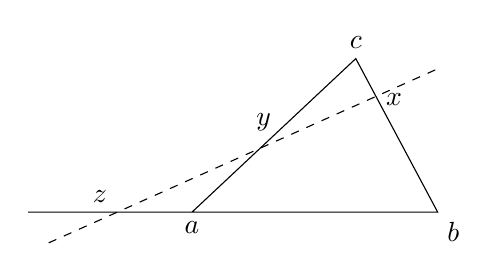
\begin{tikzpicture}[scale=1.3]
      \draw (-1,0)--(3,0)--(2.2, 1.5)--(0.6,0);
      \node[below] at (0.6, 0) {$a$};
      \node[below right] at (3,0) {$b$};
      \node[above] at (2.2, 1.5) {$c$};
      \draw[dashed] (-0.8,-0.3)--(3,1.4);
      \node[above] at (-0.3, 0) {$z$};
      \node[above] at (1.3, 0.7) {$y$};
      \node[right] at (2.4, 1.1) {$x$};
    \end{tikzpicture}\]
    Suppose that they divide these sides in the ratio 
    \[\lambda: 1, \mu: 1, \nu: 1\]
    respectively. Then, the points $x, y, z$ lie on the same line if and only if 
    \[\lambda \mu \nu = -1\]
  \end{corollary}
  \begin{proof}
  By the previous theorem, the points $x, y, z$ are linearly dependent (i.e. lies on a line) if and only if the matrix of barycentric coordinates of $x, y, z$ with respect to $a, b, c$, which is
  \begin{equation}
    \begin{pmatrix}
    0 & \frac{1}{\lambda + 1} & \frac{\lambda}{\lambda + 1} \\
    \frac{\mu}{\mu + 1} & 0 & \frac{1}{\mu + 1} \\
    \frac{1}{\nu + 1} & \frac{\nu}{\nu+1} & 0
    \end{pmatrix}
  \end{equation}
  has nonzero determinant. The determinant of the above matrix is $0$ if and only if $\lambda \mu \nu = -1$. 
  \end{proof}

  \begin{corollary}[Ceva's Theorem]
    In the triangle above, the lines $ax, by, cz$ intersect at one point if and only if 
    \begin{equation}
      \lambda \mu \nu = 1
    \end{equation}
  \end{corollary}
  \begin{proof}
    The proof can be done using barycentric coordinates. 
  \end{proof}

  \begin{theorem}
    A nonempty subset $P \subset S$ is a plane if and only if for any two distinct points $a, b \in P$, the line through $a$ and $b$ also lies in $P$. 
  \end{theorem}

  \begin{theorem}
    Given an inhomogeneous system of linear equations of form 
    \begin{equation}
      A x = b
    \end{equation}
    the set of solutions is an affine plane of dimension $n-r$, where $n$ is the number of variables and $r$ is the rank of the matrix $A$. More precisely, given that the plane is in the form $P = p_0 + U$, $p_0$ is one solution and $U$ is the set of vectors that satisfy the homogeneous system
    \begin{equation}
      Ax = 0
    \end{equation}
  \end{theorem}

  Let us observe the relative position of two planes. 

  \begin{theorem}
    Given two planes 
    \begin{align*}
      P_1 = p_1 + U_1, & P_2 = p_2 + U_2
    \end{align*}
    $P_1$ and $P_2$ intersect if and only if 
    \begin{equation}
      \overline{p_1 p_2} \subset U_1 + U_2
    \end{equation}
    where $U_1 + U_2$ is the set of all vectors of form $u_1 + u_2$, where $u_1 \in U_1, u_2 \in U_2$. 
  \end{theorem}

  Now, consider the class of functions on an affine space corresponding to the class of linear functions on a vector space. 

  \begin{definition}
    An \textbf{affine-linear} function on an affine space $S$ is a function $f: S \longrightarrow \mathbb{F}$ such that
    \begin{equation}
      f(p + x) = f(p) + \alpha (x), \;\; p \in S , x \in V
    \end{equation}
    where $\alpha$, called the \textbf{differential}, is a linear function on the vector space $V$. Let $o \in S$ be a fixed origin. By setting $p = o$, we can express an affine linear function in vectorized form as 
    \begin{equation}
      f(x) = \alpha (x) + b, \;\; b \in \mathbb{F}
    \end{equation}
    where $b = f(o)$. This implies the following coordinate form of $f$. 
    \begin{equation}
      f(x) = b + \sum_i a_i x_i
    \end{equation}
  \end{definition}

  A particular case of affine-linear functions are constant functions, where the defining characteristic is the zero differential. 

  \begin{proposition}
    Given that $\dim{S} = n$, affine-linear functions on $S$ form a $(n+1)$-dimensional subspace on the space of all linear functions on $S$. 
  \end{proposition}

  \begin{proposition}
    Barycentric coordinates are affine-linear functions. 
  \end{proposition}

  \begin{proposition}
    Let $f$ be an affine-linear function. Then
    \begin{equation}
      f \bigg( \sum_i \lambda_i p_i \bigg) = \sum_i \lambda_i f(p_i)
    \end{equation}
    for any barycentric linear combination $\sum_i \lambda_i p_i$ of points $p_1, ..., p_k$. 
  \end{proposition}

  \begin{definition}
    An affine space associated with a Euclidean vector space is called a \textbf{Euclidean affine space}. The \textbf{distance $\rho$} between two points in a Euclidean space is defined as
    \begin{equation}
      \rho(p, q) = ||\overline{pq}||
    \end{equation}
    This definition of $\rho$ satisfies the axioms of a metric space. 
  \end{definition}

\subsection{Convex Sets}

  Let $S$ be an affine space over the field of real numbers and $V$, the associated vector space. 

  \begin{definition}
    The \textbf{(closed) interval} connecting points $p, q \in S$ is the set
    \begin{equation}
      pq = \{\lambda p + (1-\lambda) q \;|\; 0 \leq \lambda \leq 1\}
    \end{equation}
    Geometrically, we can think of this as the straight line segment connecting point $p$ with point $q$. 
  \end{definition}

  \begin{definition}
    A set $M \subset S$ is \textbf{convex} if for any two points $p, q \in S$, it contains the whole interval $p, q$. 
  \end{definition}

  Clearly, the intersection of convex sets is convex. However, the union of them is not. 

  \begin{definition}
    A \textbf{convex linear combination} of points in $S$ is their barycentric linear combination with nonnegative coefficients. 
  \end{definition}

  It is clear to visualize the following proposition. 

  \begin{proposition}
    For any points $p_0, ..., p_k$ in a convex set $M \subset S$, the set $M$ also contains every convex linear combination 
    \begin{equation}
      p = \sum_i \lambda_i p_i
    \end{equation}
    Furthermore, for any set $M \subset S$, the set $\conv{M}$ of all convex linear combinations of points in $M$ is convex. 
  \end{proposition}

  \begin{definition}
    Given $M \subset S$, the set $\conv M$ is the smallest convex set containing $M$. It is called the \textbf{convex hull} of $M$. 
  \end{definition}

  \begin{definition}
    The convex hull of a system of affinely independent points $p_0, p_1, ..., p_n$ in an $n$-dimensional affine space is called the \textbf{$n$-dimensional simplex} with vertices $p_0, ..., p_n$. 
  \end{definition}

  It is clear that the interior points of a simplex is precisely the set of all points whose barycentric coordinates with respect to the vertices are all positive. 

  \begin{example}
    Here are common examples of simplices.
    \begin{enumerate}
      \item A $0$-dimensional simplex is a point. 
      \item A $1$-dimensional simplex is a closed line interval. 
      \item A $2$-dimensional simplex is a triangle. 
      \item A $3$-dimensional simplex is a tetrahedron. 
    \end{enumerate}
  \end{example}

  \begin{proposition}
    A convex set $M$ has interior points if and only if $\aff M = S$. 
  \end{proposition}

  \begin{definition}
    A convex set that has interior points is called a \textbf{convex body}. Clearly, every convex body in $n$-dimensional affine space $S$ is $n$-dimensional. 
  \end{definition}

  The set of interior points of a convex body $M$, denoted $M^\circ$, is an open convex body. 

  \begin{definition}
    For any nonconstant affine-linear function $f$ on the set $S$, let
    \begin{align*}
      H_f \equiv \{p \in S \;|\; f(p) = 0\} \\
      H^+_f \equiv \{p \in S \;|\; f(p) \geq 0\} \\
      H^-_f \equiv \{p \in S \;|\; f(p) \leq 0\}
    \end{align*}
    The set $H_f$ is a hyperplane, and $H^+_f, H^-_f$ are called \textbf{closed half spaces}. 
  \end{definition}

  \begin{definition}
    A hyperplane $H_f$ is a \textbf{supporting hyperplane} of a closed convex body $M$ if $M \subset H^+_f$ and $H_f$ contains at least one (boundary) point of $M$. The half space $H^+_f$ is then called the \textbf{supporting half-space} of $M$. 
  \end{definition}

  \begin{proposition}
    A hyperplane $H$ that passes through a boundary point of a closed convex body $M$, is supporting if and only if $H \cap M^\circ = \emptyset$. 
  \end{proposition}

  A key theorem of convex sets is the following separation theorem. 

  \begin{theorem}[Separation Theorem]
    For every boundary point of a closed convex body, there exists a supporting hyperplane passing through this point. 
  \end{theorem}

  This theorem leads to the following one. 

  \begin{theorem}
    Every closed convex set $M$ is an intersection of (perhaps infinitely many) half-spaces. 
  \end{theorem}

  \begin{definition}
    A \textbf{polyhedron} is the intersection of a finite number of half-spaces. A convex polyhedron which is also a body is called a \textbf{convex solid}. 
  \end{definition}

  \begin{example}
    A simplex with vertices $p_0, p_1, ..., p_n$ is a convex polyhedron since it is determined by linear inequalities $x_i \geq 0$ for $i = 0, 1, ..., n$, where $x_0, x_1, ..., x_n$ are barycentric coordiantes with respect to $p_0, p_1,..., p_n$. 
  \end{example}

  \begin{example}
    A convex polyhedron determined by linear inequalities $0 \leq x_i \leq 1$ for $i = 1, ..., n$, where $x_1,..., x_n$ are affine coordinates with respect ot some frame, is called an $n$-dimensional parallelopiped. 
  \end{example}

  \begin{definition}
    A point $p$ of a convex set $M$ is \textbf{extreme} if it is not an interior point of any interval in $M$. 
  \end{definition}

  \begin{theorem}
    A bounded closed convex set $M$ is the convex hull of the set $E(M)$ of its extreme points. 
  \end{theorem}

  We can create a stronger statement with the following theorem. 

  \begin{theorem}[Minkowski-Weyl Theorem]
    The following properties of a bounded set $M \subset S$ is equivalent.
    \begin{enumerate}
      \item $M$ is a convex polyhedron. 
      \item $M$ is a convex hull of a finite number of points. 
    \end{enumerate}
  \end{theorem}

  \begin{definition}
    A \textbf{face} of a convex polyhedron $M$ is a nonempty intersection of $M$ with some of its supporting hyperplanes. Given that $\dim \aff M = n$, 
    \begin{enumerate}
      \item A $0$-dimensional face is called a \textbf{vertex}. 
      \item A $1$-dimensional face an \textbf{edge}. 
      \item ...
      \item An $(n-1)$-dimensional face a \textbf{hyperface}. 
    \end{enumerate}
  \end{definition}

  Therefore, if a convex polyhedron is determined by a system of linear inequalities, we can obtain its faces by replacing some of these inequalities with equalities (in such a way that we do not get the empty set). 

  The following theorem demonstrates that in order to find its faces, it suffices to consider only the hyperplanes $H_{f_1}, ..., H_{f_m}$. 

  \begin{theorem}
    Every face $\Gamma$ of the polyhedron $M$ is of the form
    \begin{equation}
      \Gamma = M \cap \bigg( \bigcap_{j \in J} H_{f_j} \bigg)
    \end{equation}
    where $J = \{1, 2, ..., m\}$
  \end{theorem}

  \begin{proposition}
    The extreme points of a convex polyhedron $M$ are exactly its vertices. 
  \end{proposition}

  The following theorem is used often in linear programming and in optimization. 

  \begin{theorem}
    The maximum of an affine-linear function on a bounded convex polyhedron $M$ is attained at a vertex. 
  \end{theorem}

\subsection{Affine Transformations and Motions}

  Let $S$ and $S^\prime$ be affine spaces associated with vector spaces $V$ and $V^\prime$, respectively, over the same field $\mathbb{F}$. 

  \begin{definition}
    An \textbf{affine map} from the space $S$ to the space $S^\prime$ is a map $f: S \longrightarrow S^\prime$ such that
    \begin{equation}
      f(p+x) = f(p) + \varphi(x), \;\; p \in S, x \in V
    \end{equation}
    for some linear map $\varphi: V \longrightarrow V^\prime$. It follows that
    \begin{equation}
      \varphi(\overline{pq}) = \overline{f(p) f(q)}, \;\; p, q \in S
    \end{equation}
    Thus, $f$ determines the linear map $\varphi$ uniquely. Similarly, $\varphi$ is called the \textbf{differential} of $f$, denoted $df$. 
  \end{definition}

  \begin{proposition}
    Let $f: S \longrightarrow S^\prime$ and $g: S^\prime \longrightarrow S^{\prime \prime}$ be two affine maps. Then the map
    \begin{equation}
      g \circ f : S \longrightarrow S^{\prime\prime}
    \end{equation}
    is also affine. Also
    \begin{equation}
      d(g \circ f) = dg \cdot df
    \end{equation}
    where $dg$ and $df$ are the differentials of $g$ and $f$, respectively. 
  \end{proposition}

  For $\mathbb{F} = \mathbb{R}$, the differential of an affine map is a particular case of a differential of a smooth map in analysis. That is, the differential is the linear approximation of the function $f$. 

  \begin{proposition}
    An affine map is bijective if and only if its differential is bijective. 
  \end{proposition}

  \begin{definition}
    Similar to linear transformations between vector spaces, bijective affine transformations are called \textbf{isomorphisms} of affine spaces. Affine spaces are \textbf{isomorphic} if there exists an isomorphism between them. 
  \end{definition}

  \begin{corollary}
    Finite-dimensional affine spaces over the same field are isomorphic if and only if they have the same dimension. 
  \end{corollary}

  \begin{definition}
    An affine map from an affine space $S$ to itself is called an \textbf{affine transformation}. Bijective affine transformations form a group called the \textbf{affine group of $S$}, denoted $\GA(S)$. 
  \end{definition}

  It follows that given affine space $S$ with associated vector space $V$, the projection map
  \begin{equation}
    d: \GA(S) \longrightarrow \GL(V)
  \end{equation}
  is a group homomorphism. It's kernel is the group of parallel translations, called Tran$(S)$. 
  \begin{equation}
    t_a : p \mapsto p + a, \;\; a \in V
  \end{equation}

  \begin{proposition}
    For any $f \in \GA(S)$ and $a \in V$, 
    \begin{equation}
      f t_a f^{-1} = t_{df(a)}
    \end{equation}
  \end{proposition}

  \begin{definition}
    A \textbf{homothety} with the center $o$ and coefficient $\lambda$ is an affine transformation defined as
    \begin{equation}
      f( o + x ) \equiv o + \lambda x
    \end{equation}
    In its vectorized form, it is expressed
    \begin{equation}
      f(x) = \lambda x + b, \;\; b \in V
    \end{equation}
    A homothety with coefficient $-1$ is called a \textbf{central symmetry}. 
  \end{definition}

  The group of affine transformations determines the \textbf{affine geometry} of the space. The following theorem shows that all simplices are equal in affine geometry. 

  \begin{theorem}
    Let $\{p_0, ..., p_n\}$ and $\{q_0, ..., q_n\}$ be two systems of affinely independent points in an $n$-dimensional affine space $S$. Then there exists a unique affine transformation $f$ that maps $p_i$ to $q_i$ for $i = 0, 1, ..., n$. 
  \end{theorem}
  \begin{proof}
    It is easy to see once we realize that there exists a unique linear map $\varphi$ of the space $V$ that maps the basis $\{\overline{p_0 p_1}, ..., \overline{p_0 p_n}\}$ to the basis $\{\overline{q_0 q_1}, ..., \overline{q_0 q_n}\}$. If we vectorize $S$ by taking $p_0$ as the origin, the affine transformation in question has the form 
    \begin{equation}
      f(x) = \varphi(x) + \overline{p_0 q_0}
    \end{equation}
  \end{proof}

  \begin{corollary}
    In real affine geometry all parallelopipeds are equal. 
  \end{corollary}

  \begin{definition}
    A \textbf{motion} of the space $S$ is an affine transformation of $S$ whose differential is an orthogonal operator (i.e. an origin preserving isometry). Every motion is bijective. 
  \end{definition}

  Motions of a Euclidean space $S$ form a group denoted Isom$\,S$. A motion is called \textbf{proper (orientation preserving)} if its differential belongs to SO$(V)$ and improper otherwise. 

  \begin{lemma}
    The group Isom$\,S$ is generated by reflections through hyperplanes. 
  \end{lemma}

  \begin{definition}
    Let $M$ be a solid convex polyhedron in an $n$-dimensional Euclidean space. A \textbf{flag of $M$} is a collection of its faces $\{F_0, F_1, ..., F_{n-1}\}$ where $\dim{F_k} = k$ and $F_0 \subset F_1 \subset ... \subset F_{n-1}$. 
  \end{definition}

  \begin{definition}
    A convex polyhedron $M$ is \textbf{regular} if for any two of its flags, there exists a motion $f \in$ Sym$\,M$ mapping the first to the second, where 
    \begin{equation}
      \text{Sym}\,M \equiv \{f \in \text{Isom}\,S \;|\; f(M) = M \}
    \end{equation}
  \end{definition}

  Two dimensional regular polyhedra are the ordinary \textbf{regular polygons}. Their symmetry groups are known as the dihedral groups.

  Three dimensional regular polyhedra are \textbf{Platonic solids}, which are the regular tetrahedron, cube, octahedron, dodecahedron, and icosahedron. 

  \begin{definition}
    A real vector space $V$ with a fixed symmetric bilinear function $\alpha$ of signature $(k, l)$, where $k, l > 0$ and $\dim{V} = k+l$, is called the \textbf{pseudo-Euclidean vector space} of signature $(k, l)$. The group of $\alpha$-preserving linear transformations of $V$ is called the \textbf{pseudo-orthogonal group} and is denoted O$(V, \alpha)$. In an orthonormal basis, the corresponding matrix group is denoted $O{k,l}$. 
  \end{definition}

\subsection{Quadrics}

  Planes are the simplest objects of affine and Euclidean geometry, which are determined by systems of linear equations. The second simplest are quadratic functions. These types of objects are studied futher in algebraic geometry. 

  \begin{definition}
    An \textbf{affine-quadratic function} on an affine space $S$ is a function $Q: S \longrightarrow \mathbb{F}$ such that its vectorized form is
    \begin{equation}
      Q(x) = q(x) + l(x) + c
    \end{equation}
    for a quadratic function $q$, linear function $l$, and constant $c$. 
  \end{definition}

\subsection{Projective Spaces}

  \begin{definition}
    An $n$-dimensional \textbf{projective space $PV$} over a field $\mathbb{F}$ is the set of one-dimensional subspaces of an $(n+1)$-dimensional vector space $V$ over $\mathbb{F}$. For every $(k+1)$-dimensional subspace $U \subset V$, the subset $PU \subset PV$ is called a $k$-dimensional \textbf{plane} of the space $PV$. 
    \begin{enumerate}
      \item $0$-dimensional planes are the points of $PV$. 
      \item $1$-dimensional planes are called \textbf{lines}
      \item ...
      \item $(n-1)$-dimensional planes are called \textbf{hyperplanes}
    \end{enumerate}
  \end{definition}

  \begin{definition}
    $\mathbb{RP}^1$ is called the real projective line, which is topologically equivalent to a circle. 
  \end{definition}

  \begin{example}
    The real projective space of $\mathbb{R}^2$ is the set of all lines that pass through the origin. It is denoted $\mathbb{R P}^2$ and called the \textbf{real projective plane}. 
  \end{example}

  \begin{example}
    $\mathbb{RP}^3$ is diffeomorphic to SO$(3)$. 
  \end{example}

  \begin{example}
    The space $\mathbb{RP}^n$ is formed by taking the quotient of $\mathbb{R}^{n+1} \setminus \{0\}$ under the equivalence relation 
    \begin{equation}
      x \sim \lambda x \text{ for all real numbers } \lambda \neq 0
    \end{equation}
    The set of these equivalence classes is isomorphic to $\mathbb{RP}^n$. 
  \end{example}


\section{Representations}

  We will assume that $V$ is a finite-dimensional vector space over field $\mathbb{C}$. 

  \begin{definition}
    The \textbf{general linear group} of vector space $V$, denoted $\GL(V)$, is the group of all automorphisms of $V$ to itself. The \textbf{special linear group} of vector space $V$, denoted $\SL(V)$ is the subgroup of automorphisms of $V$ with determinant $1$. 
  \end{definition}

  When studying an abstract set, it is often useful to consider the set of all maps from this abstract set to a well known set (e.g. $\GL(V)$). 

  \begin{definition}
    A \textbf{representation} of an (algebraic) group $\mathcal{G}$ is a homomorphism 
    \begin{equation}
      \rho: G \longrightarrow \GL(V)
    \end{equation}
    for some vector space $V$. That is, given an element $g \in \mathcal{G}$, $\rho(g) \in \GL (V)$, meaning that $\rho(g)(v) \in V$. Additionally, since it is a homomorphism, the algebraic structure is preserved. 
    \begin{equation}
      \rho(g_1 \cdot g_2) = \rho(g_1) \cdot \rho(g_2)
    \end{equation}
    where $\cdot$ on the left hand side is the abstract group multiplication while the $\cdot$ on the right hand side is matrix multiplication. To shorten the notation, we will denote 
    \begin{equation}
      g v = \rho(g) v, \; v \in V
    \end{equation}
    Since $\rho$ is a group morphism, we have 
    \begin{equation}
      g_2 (g_1 v) = (g_2 g_1) v \; \iff \rho(g_2) \big( \rho(g_1) (v) \big) = \big( \rho(g_2) \rho(g_1) \big) (v)
    \end{equation}
    Additionally, since $g$ (that is, $\rho(g)$) is a linear map, 
    \begin{equation}
      g(\lambda_1 v_1 + \lambda_2 v_2) = \lambda_1 g v_1 + \lambda_2 g v_2
    \end{equation}
    Usually, we refer to the map as the representation, but if the map is well-understood, we just call the vector space $V$ the representation and say that the group acts on this vector space. 
  \end{definition}

  \begin{example}
    The group $\GL(2, \mathbb{C})$ can be represented a by the vector space $\mathbb{C}^2$, or explicitly, by the group of $2 \times 2$ matrices over $\mathbb{C}$ with nonzero determinant.
    \begin{equation}
      \GL(2, \mathbb{C}) \xmapsto{id} \text{Mat}(2, \mathbb{C})
    \end{equation}
    This is a trivial representation. 
  \end{example}

  We now show a nontrivial representation of $\GL(2, \mathbb{C})$. 

  \begin{example}
    We take Sym$^2 \mathbb{C}^2$, the second symmetric power of $\mathbb{C}^2$. Note that given a basis $x_1, x_2 \in \mathbb{C}^2$, the set
    \begin{equation}
      \{x_1 \odot x_1, x_1 \odot x_2, x_2 \odot x_2\}
    \end{equation}
    forms a basis of Sym$^2 \mathbb{C}^2 \implies \dim\,$Sym$^2 \mathbb{C}^2 = 3$. So, we want to represent $\GL(2, \mathbb{C})$ by associating its element with elements of $\GL(Sym^2 \mathbb{C}^2)$. More concretely, we are choosing to represent a $2 \times 2$ matrix over $\mathbb{C}$ with a $3 \times 3$ matrix group (since $\GL(Sym^2 \mathbb{C}^2) \simeq \GL(3, \mathbb{C})$. Clearly,
    \begin{align*}
      & \rho(g) (x_1 \odot x_1) = g(x_1) \odot g(x_1) \in Sym^2 \mathbb{C}^2 \\
      & \rho(g) (x_1 \odot x_2) = g(x_1) \odot g(x_2) \\
      & \rho(g) (x_2 \odot x_2) = g(x_2) \odot g(x_2)
    \end{align*}
    To present this in matrix form, let us have an element in $\GL (2, \mathbb{C})$
    \begin{equation}
      \mathcal{A} \equiv \begin{pmatrix}
      a & b \\
      c & d
      \end{pmatrix}
    \end{equation}
    We evaluate the corresponding representation in $\GL( Sym^2 \mathbb{C}^2)$. Using the identities above, we have 
    \begin{align*}
      \rho(g) (x_1 \odot x_1) & = g(x_1) \odot g(x_1) \\
      & = (a x_1 + c x_2) \odot (a x_1 + c x_2) \\
      & = a^2 x_1 \odot x_1 + 2ac x_1 \odot x_2 + c^2 x_2 \odot x_2 \\
      \rho(g) (x_1 \odot x_2) & = g(x_1) \odot g(x_2) \\
      & = (a x_1 + c x_2) \odot (b x_1 + d x_2) \\
      & = ab x_1 \odot x_1 + (ad + bc) x_1 \odot x_2 + cd x_2 \odot x_2 \\
      \rho(g) (x_2 \odot x_2) & = g(x_2) \odot g(x_2) \\
      & = (b x_1 + d x_2) \odot (b x_1 + d x_2) \\
      & = b^2 x_1 \odot x_1 + 2bd x_1 \odot x_2 + d^2 x_2 \odot x_2
    \end{align*}
    And this completely determines the matrix. So, 
    \begin{equation}
      \rho \begin{pmatrix}
      a&b\\c&d
      \end{pmatrix} = \begin{pmatrix}
      a^2&ab&b^2\\2ac&ad+bc&2bd\\c^2&cd&d^2
      \end{pmatrix}
    \end{equation}
    is the $3 \times 3$ representation of $\mathcal{A}$ in $\GL(Sym^2 \mathbb{C}^2)$. 
  \end{example}

  We continue to define maps between two representations of $\mathcal{G}$. 

  \begin{definition}
    A \textbf{morphism} between 2 representations 
    \begin{align*}
      & \rho_1: \mathcal{G} \longrightarrow \GL(V_1) \\
      & \rho_2: \mathcal{G} \longrightarrow \GL(V_2) 
    \end{align*}
    of some group but not necessarily the same vector space is a linear map $f: V_1 \longrightarrow V_2$ that is \textbf{compatible} with the group action. That is, $f$ satisfies the property that for all $g \in \mathcal{G}$
    \begin{equation}
      f \circ g = g \circ f
    \end{equation}
    Again, we use the shorthand notation that $g = \rho(g)$, meaning that the statement above really translates to $ f \circ \rho(g) = \rho(g) \circ f$. This is equivalent to saying that the following diagram commutes. 
    \[\begin{tikzcd}
    V_1 \arrow{r}{\rho_1(g)} \arrow{d}{f} & V_1 \arrow{d}{f} \\
    V_2 \arrow{r}{\rho_2 (g)} & V_2
    \end{tikzcd}\]
  \end{definition}

  \begin{definition}
    Let $V$ be a representation of $\mathcal{G}$. A \textbf{subrepresentation} is a subspace $W \subset V$ such that for all $g \in \mathcal{G}$ and for all $w \in W$, 
    \begin{equation}
      \rho(g)(w) \in W
    \end{equation}
  \end{definition}

  \begin{example}
    $V$ and $\{0\}$ are always subrepresentations of $V$. 
  \end{example}

  We now introduce the "building blocks" of all representations. 
  \begin{definition}
    A representation $W$ is \textbf{irreducible representation} if $\{0\}$ and $W$ are the only subrepresentations of $W$. 
  \end{definition}

  \begin{lemma}[Schur's Lemma]
    Let $V_1, V_2$ be irreducible representations and let $f: V_1 \longrightarrow V_2$ be a morphism (of representations). Then, either
    \begin{enumerate}
      \item $f$ is an isomorphism. 
      \item $f = 0$
    \end{enumerate}
    Furthermore, any 2 isomorphisms differ by a constant. That is, 
    \begin{equation}
      f_1 = \lambda f_2
    \end{equation}
  \end{lemma}
  \begin{proof}
    $\ker{f}$ is clearly a vector space. Furthermore, it is a subrepresentation (since it is a subspace of $V_1$) $\implies \ker{f} = V$ or $\ker{f} = 0$. If $\ker{f} = V$, then $f = 0$ and the theorem is satisfied. If $\ker{f} = 0$, then $f$ is injective, and $\im{f}$ is a subrepresentation of $V_2 \implies \im{f} = 0$ or $\im{f} = V_2$. But $\im{f} \neq 0$ since $f$ is injective, so $\im{f} = V_2 \implies f$ is surjective $\implies f$ is bijective, that is, $f$ is an isomorphism of vector spaces. So, the inverse $f^{-1}$ exists, and this map $f^{-1}$ satisfies
    \begin{equation}
      f^{-1} \circ \rho_2(g) = \rho_1 (g) \circ f^{-1}
    \end{equation}
    To prove the second part, without loss of generality, assume that the first isomorphism is the identity mapping. That is, 
    \begin{equation}
      f_1 = id
    \end{equation}
    Since we are working over the field $\mathbb{C}$, we can find an eigenvector of $f_2$. That is, there exists a $v \in V_1$ such that 
    \begin{equation}
      f_2 (v) = \lambda v
    \end{equation}
    Now, we define the map
    \begin{equation}
      f: V_1 \longrightarrow V_2, \; f \equiv f_2 - \lambda f_1
    \end{equation}
    Clearly, $\ker{f} \neq 0$, since $v \in \ker{f}$. That is, we have a map $f$ between 2 irreducible representations that has a nontrivial kernel. This means that $f = 0 \implies f_2 = \lambda f_1$.  
  \end{proof}

  \begin{theorem}[Mache's Theorem]
    Let $V$ be finite dimensional, with $\mathcal{G}$ a finite group. Then, $V$ can be decomposed as 
    \begin{equation}
      V = \bigoplus_{i} V_i
    \end{equation}
    where each $V_i$ is an irreducible representation of $\mathcal{G}$. 
  \end{theorem}
  \begin{proof}
    By induction on dimension, it suffices to prove that if $W$ is a subrepresentation of $V$, then there exists a subrepresentation $W^\prime \subset V$ such that $W \oplus W^\prime = V$. So, if $V$ isn't an irreducible representation, it can always be decomposed into smaller subrepresentations $W$ and $W^\prime$ that direct sum to $V$. Now, we define the canonical (linear) projection 
    \begin{equation}
      \pi: V \longrightarrow W
    \end{equation}
    Then, we define the new map 
    \begin{equation}
      \Tilde{\pi}: V \longrightarrow W, \; \Tilde{\pi}(v) \equiv \frac{1}{|\mathcal{G}|} \sum_{g \in \mathcal{G}} \rho(g)\big|_W \circ \pi \circ \rho(g)^{-1}
    \end{equation}
    This "averaging" of the group elements are done so that this mapping is a map of representations. This implies that 
    \begin{equation}
      V = W \oplus \ker{\Tilde{\pi}}
    \end{equation}
    meaning that $V$ can indeed be decomposed into direct sums of subrepresentations. 
  \end{proof}


\section{Lie Groups and Lie Algebras}

  \begin{definition}
    A \textbf{Lie group} is a group $\mathcal{G}$ that is also a finite-dimensional smooth manifold, in which the group operations of multiplication and inversion are smooth maps. Smoothness of the group multiplication
    \begin{equation}
      \mu: \mathcal{G} \times \mathcal{G} \rightarrow \mathcal{G}, \; \mu(x, y) = x y
    \end{equation}
    means that $\mu$ is a smooth mapping of the product manifold $\mathcal{G} \times \mathcal{G}$ into $\mathcal{G}$. These two requirements can be combined to the single requirement that tahe mapping 
    \begin{equation}
      (x, y) \mapsto x^{-1} y
    \end{equation}
    be a smooth mapping of the product manifold into $\mathcal{G}$. 
  \end{definition}

  \begin{definition}
    A \textbf{Lie Algebra} is a vector space $\mathfrak{g}$ with an operation called the \textbf{Lie Bracket} 
    \begin{equation}
      [\cdot, \cdot]: \mathfrak{g} \times \mathfrak{g} \rightarrow \mathfrak{g}
    \end{equation}
    Satisfying
    \begin{enumerate}
      \item Bilinearity: $[ax + by, z] = a[x,z] + b[y,z], \; [z, ax + by] = a[z, x] + b[z,y]$
      \item Anticommutativity: $[x,y] = -[y,x]$
      \item Jacobi Identity: $[x,[y,z]] + [y,[z,x]] + [z,[x,y]] = 0$
    \end{enumerate}
    Clearly, this implies that $\mathfrak{g}$ is a nonassociative algebra. Note that a Lie Algebra does not necessarily need to be an algebra in the sense that there needs to be multiplication operation that is closed in $\mathfrak{g}$. 
  \end{definition}

  \begin{example}
    A common example of a Lie Braket in the algebra of matrices is defined
    \begin{equation}
      [A, B] \equiv AB - BA
    \end{equation}
    called the \textbf{commutator}. Note that in this case, the definition of the Lie bracket is dependent on the definition of the matrix multiplication. Without defining the multiplication operation, we wouldn't know what $AB$ or $BA$ means. Therefore, we see that the Lie algebra of $n \times n$ matrices has three operations: matrix addition, matrix multiplication, and the commutator (along with scalar multiplication). But in general, it is not necessary to have that multiplication operation for abstract Lie algebras. $\mathfrak{g}$ just needs to be a vector space with the bracket.  
  \end{example}

  \begin{example}
    The set of all symmetric matrices is a vector space, but it is \textbf{not} a Lie algebra since the commutator $[A,B]$ is not symmetric unless $A B = B A$. 
  \end{example}

  We will first talk about groups of matrices as a more concerete example before we get into abstract Lie groups. Recall that the matrix exponential map is defined
  \begin{equation}
    exp: \text{Mat}(n, \mathbb{C}) \rightarrow \text{mat}(n, \mathbb{C}), \; exp(A) = e^A = \sum_{p \geq 0} \frac{A^p}{p!}
  \end{equation}
  Note that this value is always well defined. This lets us define
  \begin{equation}
    exp(t A) \equiv e^{t A} \equiv I + tA + \frac{1}{2} t^2 A^2 + \frac{1}{3!} t^3 A^3 + ... 
  \end{equation}
  where if $t$ is small, we can expect a convergence. Note that exp maps addition to multiplication. That is, we can interpret it as a homomorphism from 
  \begin{equation}
    exp: \mathfrak{g} \rightarrow \mathcal{G}
  \end{equation}
  where $\mathfrak{g}$ is the Lie algebra and $\mathcal{G}$ is the Lie group (which we will treat just as a matrix group). To find the inverse of the exponential map, we can take the derivative of $e^{tA}$ at $t=0$. That is, 
  \begin{align*}
    \bigg(\frac{d}{d t} e^{tA} \bigg) \bigg|_{t=0} & = \bigg(\sum_{k=0}^\infty \frac{1}{k!} t^k A^{k+1} \bigg) \bigg|_{t=0} = A
  \end{align*}
  So, the mapping
  \begin{equation}
    \frac{d}{dt} \bigg|_{t=0}: \mathcal{G} \rightarrow \mathfrak{g}
  \end{equation}
  maps the Lie group back to the algebra. We can interpret this above mapping by visualizing the Lie Algebra as a tangent (vector) space of the abstract Lie group $\mathcal{G}$ at the identity element of the Lie group. The visualization below isn't the most abstract one, but it may help:

  \begin{figure}[H]
    \centering 
    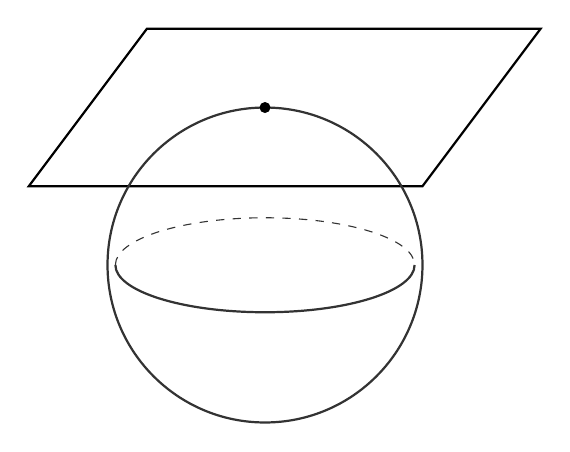
\begin{tikzpicture}[scale=1]
      % Define colors
      \colorlet{spherecol}{black!80}
      \colorlet{arrowcol}{cyan!70!blue}
      
      % Draw the tangent plane (Lie Algebra)
      \draw[thick] (-1.5,3) -- (3.5,3) -- (2,1) -- (-3,1) -- cycle;
      
      % Draw the sphere (Lie Group)
      \draw[spherecol, thick] (0,0) circle (2cm);
      \draw[spherecol, thick] (-1.9,0) arc (180:360:1.9cm and 0.6cm);
      \draw[spherecol, dashed] (-1.9,0) arc (180:0:1.9cm and 0.6cm);
      
      % Identity element
      \fill (0,2) circle (0.07cm);
    \end{tikzpicture}
    \caption{The Lie algebra can be visualized as the tangent space at the identity.} 
    \label{fig:lie_algebra_tangent_space}
  \end{figure}

  For example, say that the Lie group $\mathcal{G}$ is a unit circle in $\mathbb{C}$, then the Lie algebra of $\mathcal{G}$ is the tangent space at the identity $1$, which can be identified as the imaginary line in the complex plane $\{i t \; | \; t \in \mathbb{R}\}$, with 
  \begin{equation}
    i t \mapsto exp(it) \equiv e^{it} \equiv \cos{t} + i \sin{t}
  \end{equation}

  \begin{center}
    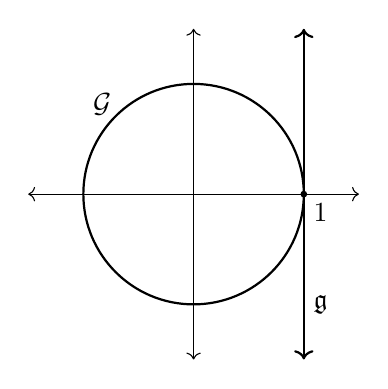
\begin{tikzpicture}[scale=0.7]
      \draw[thick] (0,0) circle (2);
      \node[below right] at (-2,2) {$\mathcal{G}$};
      \draw[<->] (-3,0)--(3,0);
      \draw[<->] (0,-3)--(0,3);
      \draw[fill] (2,0) circle (0.05);
      \node[below right] at (2,0) {$1$};
      \draw[thick, <->] (2,-3)--(2,3);
      \node[right] at (2,-2) {$\mathfrak{g}$};
    \end{tikzpicture}
  \end{center}
  So, analyzing the Lie group by looking at its Lie algebra turns a nonlinear problem to a linear one; this is called a \textbf{linearization} of the Lie group. The existence of this exponential map is one of the primary reasons that Lie algebras are useful for studying Lie groups. 

  \begin{example}
    The exponential map 
    \begin{equation}
      exp: \mathbb{R} \rightarrow \mathbb{R}^+, \; x \mapsto e^x
    \end{equation}
    is a group homomorphism that maps $(\mathbb{R}, +)$ to $(\mathbb{R}^+, \times)$. This means that $\mathbb{R}$ is the Lie algebra of the Lie group $\mathbb{R}^+$. 
  \end{example}

  \begin{theorem}
    If $A$ and $B$ are commuting square matrices, then 
    \begin{equation}
      e^{A + B} = e^A \, e^B
    \end{equation}
    In general, the solution $C$ to the equation
    \begin{equation}
      e^{A} \, e^B = e^C
    \end{equation}
    is given by the \textbf{Baker-Campbell-Hausdorff formula}, defined
    \begin{equation}
      C = A + B + \frac{1}{2}[A,B] + \frac{1}{12} [A,[A,B]] - \frac{1}{12} [B,[A,B]] + ...
    \end{equation}
    consisting of terms involving higher commutators of $A$ and $B$. The full series is much too complicated to write, so we ask the reader to be satisfied with what is shown. 
  \end{theorem}

  The BCH formula is messy, but it allows us to compute products in the Lie Group as long as we known the commutators in the Lie Algebra. 

  Therefore, we can describe the process of constructing a Lie group from a Lie Algebra (which a vector space) as such. We take a vector space $V$ and endow it the additional bracket operation. We denote this as
  \begin{equation}
    \mathfrak{g} \equiv (V, [\cdot, \cdot])
  \end{equation}
  Then, we take every element of $\mathfrak{g}$ and apply the exponential map to them to get an another set $\mathcal{G}$. We then endow a group structure on $\mathcal{G}$ by defining the multiplication as 
  \begin{equation}
    \cdot: \mathcal{G} \times \mathcal{G} \rightarrow \mathcal{G}, \; e^A \cdot e^B = e^{A * B}
  \end{equation}
  where $A*B$ is defined by the BCH formula up to a certain $k$th order. Since the $*$ operation is completely defined by the bracket in the Lie algebra, it tells us how to multiply in the Lie group. This process can be made more abstractly, depending on what $A, B$ and $[\cdot,\cdot]$ is, beyond matrices. 

\subsection{Lie Algebras of Classical Lie Groups}

  \begin{definition}[General Linear Group]
    The \textbf{general linear group}, denoted GL$(V)$, is the set of all bijective linear mappings from $V$ to itself. Similarly, GL$_{n}(\mathbb{F})$, or GL $(n, \mathbb{F})$ is the set of all nonsingular $n \times n$ matrices over the field $\mathbb{F}$. Due to the same dimensionality of the following spaces, it is clear that GL$(V) \simeq$ GL$(\mathbb{F}^{n}) \simeq$ GL$_{n}(\mathbb{F})$. The \textbf{special linear group}, denoted SL$_{n} (\mathbb{F})$ or SL$(n, \mathbb{F})$, is the set of $n\times n$ matrices a with determinant $1$. SL$_{n}(\mathbb{F})$ is a subgroup of GL$_{n}(\mathbb{F})$, which is a subset of the ring of all $n \times n$ matrices over field $\mathbb{F}$, denoted $\mathbb{L}_{n}(\mathbb{F})$. 
  \end{definition}

  \begin{definition}[Translation Group]
    The group of all translations in the space $V$ is denoted Tran$\,V$. Its elements are usually denoted as $t_{u}$, where $u$ is the vector that is being translated by. It can also be interpreted as shifting the origin by $-u$. It is clear that Tran$\,V \simeq V$. 
  \end{definition}

  \begin{definition}[General Affine Group]
    The \textbf{general affine group} is the pair of all transformations
    \begin{equation}
      \text{GA} (V) \equiv \text{Tran}(V) \times \text{GL}(V)
    \end{equation}
  \end{definition}

  \begin{definition}[Isometries]
    The \textbf{Euclidean group} of \textbf{isometries} in the Euclidean space $\mathbb{E}^{n}$ (with the Euclidean norm), denoted Isom$\, \mathbb{E}^{n}$ or $\mathbb{E}(n)$, consists of all distance-preserving bijections from $\mathbb{E}^{n}$ to itself, called \textbf{motions} or \textbf{rigid transformations}. It consists of all combinations of rotations, reflections, and translations. The \textbf{special Euclidean group} of all isometries that preserve the \textbf{handedness} of figures is denoted $\mathbb{SE}(n)$, which is comprised of all combinations rotations and translations called \textbf{rigid motions} or \textbf{proper rigid transformations}.
  \end{definition}

  \begin{definition}[Orthogonal Group]
    The \textbf{orthogonal group}, denoted $\O(n)$, consists of all isometries that preserve the origin, i.e. consists of rotations and reflections. The \textbf{special orthogonal group}, denoted SO$(n)$, is a subgroup of O$(n)$ consisting of only rotations. We can see that 
    \begin{equation}
      \text{O}(n)=\frac{\text{Isom}\, \mathbb{E}^{n}}{\text{Tran}\,V}
    \end{equation}
  \end{definition}

  \begin{definition}[Transitive]
    A transformation group $G$ is called \textbf{transitive} if for any $x, y \in X$, there exists a $\phi \in G$ such that $y = \phi(x)$. 
  \end{definition}

  \begin{example}
    Tran$(V)$ and GA$(V)$ are transitive groups. 
  \end{example}

  \begin{definition}[Congruence Classes]
    Let $X$ be a set and $G$ its transformation group on $X$. The way we define $G$ determines the \textbf{geometry} of $X$. More specifically, a figure $F_{1} \subset X$ is \textbf{equivalent} or \textbf{congruent} to $F_{2} \subset X$ iff there exists $\phi \in G$ such that $F_{2} = \phi (F_{1})$ (or equivalently, $F_{1} = \phi (F_{2})$). This is an equivalence relation since
    \begin{enumerate}
      \item $F \sim F$. 
      \item $F \sim H \implies H \sim F$. 
      \item $F \sim H, H \sim K \implies F \sim K$
    \end{enumerate}
    Two figures that are in the same equivalence class are known to be \textbf{congruent} with respect to the geometry of $X$ induced by $G$. 
  \end{definition}

  Clearly, if two figures are congruent in Euclidean geometry, then they are congruent in Affine geometry, since E$(n) \subset$ GA$(n)$. 


\subsubsection[Lie Algebras of SL(2, R) and SL(2, C)]{Lie Algebras of $\SL(2, \mathbb{R})$ and $\SL(2, \mathbb{C})$}

  Given the group $\SL(2, \mathbb{R})$, there must be a corresponding Lie algebra of matrices such that $g = e^A \in \SL(2, \mathbb{R})$. We attempt to find this Lie algebra. Let $g \in \SL(2, \mathbb{R})$, with $g = e^A$. So, if $\det{g} = 1$, what is the corresponding restriction on $A$ in the algebra? We use the following theorem. 

  \begin{theorem}
    \begin{equation}
      \det{(e^A)} = e^{\Tr{(A)}}
    \end{equation}
  \end{theorem}
  \begin{proof}
    Put $A$ in Jordan Normal Form: $A = S^{-1} J S \implies A^n = S^{-1} J^n S \implies exp(A) = S^{-1} exp(A) S \implies \det{(exp(A))} = \det{e^J}$. But since $J$ is upper trianglar, $J^n$ is upper triangular $\implies e^J$ is upper triangular, which implies that 
    \begin{equation}
      \det{e^J} = \prod_i e^{\lambda_i} = e^{\Tr{(J)}} = e^{\Tr{(A)}}
    \end{equation}
    since trace is invariant under a change of basis. 
  \end{proof}

  So, $\det{(e^A)} = 1 \implies \Tr{(A)} = 2 \pi i n$ for $n \in \mathbb{Z}$. Since we want to component connected to the identity, we choose $n=0$ meaning that $\Tr{(A)} = 0$. And we are done. That is, the Lie algebra of $\SL(2, \mathbb{R})$ consists of traceless $2 \times 2$ matrices, denoted $\mathfrak{sl}_2 \mathbb{R}$. $\mathfrak{sl}_2 \mathbb{R}$ has basis (chosen arbitrarily) 
  \begin{equation}
    \bigg\{ H = \begin{pmatrix}
    1&0\\0&-1
    \end{pmatrix}, X = \begin{pmatrix}
    0&1\\0&0
    \end{pmatrix}, Y = \begin{pmatrix}
    0&0\\1&0
    \end{pmatrix}\bigg\}
  \end{equation}
  and the identity in the Lie algebra is the zero matrix, which translates to the $2 \times 2$ identity matrix in the Lie group. 
  \begin{equation}
    exp \begin{pmatrix}
    0&0\\0&0
    \end{pmatrix} = I
  \end{equation}
  We must not forget to define the bracket structure in $\mathfrak{sl}_2 \mathbb{R}$, so we define it as the commutator, which gives the identity
  \begin{align*}
    & [H,X] = HX - XH = 2X \\
    & [H,Y] = HY - YH = -2Y \\
    & [X,Y] = XY - YX = H
  \end{align*}
  Note that regular matrix multiplication is not closed within this Lie algebra. For example, 
  \begin{equation}
    X Y = \begin{pmatrix}
    1&0\\0&0
    \end{pmatrix}
  \end{equation}
  is clearly not traceless. However, the bracket operation keeps the matrices within this traceless condition (and thus, within this algebra), so you can't just stupidly multiply matrices together in a Lie algebra. Remember that regular matrix multiplication does not have anything to do with the Lie bracket and does not apply to this group. This algebra also simplifies the multiplicative inverse of a group to a simple additive inverse, making calculations easier. 

  Similarly, the Lie algebra of $\SL(2, \mathbb{C})$ also has the same basis 
  \begin{equation}
    \bigg\{ H = \begin{pmatrix}
    1&0\\0&-1
    \end{pmatrix}, X = \begin{pmatrix}
    0&1\\0&0
    \end{pmatrix}, Y = \begin{pmatrix}
    0&0\\1&0
    \end{pmatrix}\bigg\}
  \end{equation}
  but we choose the field to be $\mathbb{C}$, meaning that we take complex linear combinations rather than real linear ones. 

\subsubsection[Lie Algebra of SU(2)]{Lie Algebra of \(\SU(2)\)}

  $g \in $ SU$(2) \implies \det{g} = 1 \implies \Tr{A} = 0$. We also see that by definition $e^A$, 
  \begin{equation}
    (e^A)^\dagger = e^{A^\dagger} \text{ and } (e^A)^{-1} = e^{-A}
  \end{equation}
  which implies that $A^\dagger = - A$. That is, the unitary condition implies that the Lie algebra elements in $\mathfrak{su}(2)$ are traceless, anti-self adjoint $2 \times 2$ matrices over $\mathbb{C}$. 

  \begin{definition}
    The \textbf{Pauli matrices} are the three matrices
    \begin{equation}
      \bigg\{ \sigma_x = \begin{pmatrix}
      0&1\\1&0
      \end{pmatrix}, \sigma_y = \begin{pmatrix}
      0&-i\\i&0
      \end{pmatrix}, \sigma_z = \begin{pmatrix}
      1&0\\0&-1
      \end{pmatrix}\bigg\}
    \end{equation}
    Note that with some calculation, 
    \begin{align*}
      & [\sigma_x, \sigma_y] = 2 i \sigma_z \\
      & [\sigma_y, \sigma_z] = 2 i \sigma_x \\
      & [\sigma_z, \sigma_x] = 2 i \sigma_y
    \end{align*}
  \end{definition}

  To identify the basis of $\mathfrak{su}(2)$, we take the Pauli matrices and let 
  \begin{align*}
    & A_x \equiv - \frac{i}{2} \sigma_x = \begin{pmatrix} 0&-i/2\\-i/2&0 \end{pmatrix} \\
    & A_y \equiv - \frac{i}{2} \sigma_y = \begin{pmatrix}0&-1/2\\1/2&0\end{pmatrix} \\
    & A_z \equiv -\frac{i}{2} \sigma_z = \begin{pmatrix}-i/2&0\\0&i/2\end{pmatrix}
  \end{align*} 
  be the basis of $\mathfrak{su}(2)$. Clearly, $A_x, A_y, A_z$ are all traceless, anti-self adjoint $2 \times 2$ matrices. Moreover, they also satisfy
  \begin{align*}
    & [A_x, A_y] = A_z \\
    & [A_y, A_z] = A_x \\
    & [A_z, A_x] = A_y
  \end{align*}
  However, note that the algebra $\mathfrak{su}(2)$ consists of all \textbf{real} linear combinations of $A_x, A_y, A_z$. That is, $\mathfrak{su}(2)$ is a 3 dimensional \textbf{real} vector space, even though it has basis elements containing complex numbers. 

  However, we can always complexify this space by simply replacing real scalar multiplication in $\mathfrak{su}(2)$ with complex scalar multiplication. By complexifying $\mathfrak{su}(2)$, the Lie group SU$(2)$ formed by taking the exponential map on this complexified space is actually identical to $\SL(2, \mathbb{C})$. Indeed, this is true because first, the basis $\{H, X, Y\}$ of $\mathfrak{sl}_2 \mathbb{C}$ and the basis $\{A_x, A_y, A_z\}$ of $\mathfrak{su}(2)$ span precisely the same subspace in the vector space Mat$(2, \mathbb{C})$, meaning that the two Lie algebras are the same vector space. Secondly, the bracket operation $[\cdot, \cdot]$ in both $\mathfrak{sl}_2 \mathbb{C}$ and $\mathfrak{su}(2)$ are equivalent since the operation defined to be the commutator in both cases, resulting in the similarities in the bracket behaviors. 
  \begin{align*}
    [H,X] = 2X & \iff [A_x, A_y] = A_z \\
    [H,Y] = - 2Y & \iff [A_y, A_z] = A_x\\
    [X,Y] = H & \iff  [A_z, A_x] = A_y 
  \end{align*}
  Therefore, the complexification of SU$(2)$ and $\SL(2, \mathbb{R})$ both leads to the construction of $\SL(2, \mathbb{C})$. 

  \begin{center}
    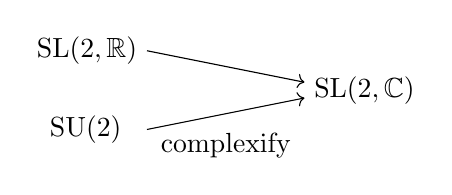
\begin{tikzpicture}
      \node[left] at (0,0.5) {$\SL(2, \mathbb{R})$};
      \node[left] at (-0.2,-0.5) {SU$(2)$};
      \node[right] at (2,0) {$\SL(2,\mathbb{C})$};
      \draw[->] (0,0.5)--(2,0.1);
      \draw[->] (0,-0.5)--(2,-0.1);
      \node at (1,-0.7) {complexify};
    \end{tikzpicture}
  \end{center}
  We can interpret the "real forms" of $\SL(2, \mathbb{C})$ as "slices" of some complex group. However, this does not mean that the real version of these groups are equal. That is, 
  \begin{equation}
    \SL(2, \mathbb{R}) \neq \text{SU}(2)
  \end{equation}

\subsubsection{Lie Algebra of SO(3)}

  It is easy to see that for SO$(2)$, it is easy to see that its Lie algebra $\mathfrak{so}(2)$ has 
  \begin{equation}
    \bigg\{ \begin{pmatrix}
    0&-1\\1&0
    \end{pmatrix}\bigg\}
  \end{equation}
  as its only basis, since 
  \begin{equation}
    exp  \bigg( \begin{pmatrix}
    0&-1\\1&0
    \end{pmatrix} \theta \bigg) = \begin{pmatrix}
    \cos{\theta} & - \sin{\theta} \\
    \sin{\theta} & \cos{\theta}
    \end{pmatrix}
  \end{equation}
  meaning that the dimension of SO$(2)$ is $1$. By adding a component, we can get a rotation in $\mathbb{R}^3$. 
  \begin{align*}
    & R_x = \begin{pmatrix}0&0&0\\0&0&-1\\0&1&0\end{pmatrix} \implies e^{R_x} = \begin{pmatrix}
    1&0&0\\ 0&\cos{\theta}&-\sin{\theta}\\0&\sin{\theta}&\cos{\theta}
    \end{pmatrix}\\
    & R_y = \begin{pmatrix}0&0&1\\0&0&0\\-1&0&0\end{pmatrix} \implies e^{R_y} = \begin{pmatrix}
    \cos{\theta} & 0 & -\sin{\theta}\\ 0&1&0 \\
    \sin{\theta}& 0 & \cos{\theta} \end{pmatrix} \\
    & R_z = \begin{pmatrix}0&-1&0\\1&0&0\\0&0&0\end{pmatrix} \implies e^{R_z} = \begin{pmatrix}
    \cos{\theta} & -\sin{\theta} & 0\\
    \sin{\theta}& \cos{\theta} & 0 \\ 0 & 0 & 1\end{pmatrix}
  \end{align*}
  That is, $e^{R_x}, e^{R_y}$, and $e^{R_z}$ generates a rotation around the $x, y$, and $z$ axis, respectively, which completely generates the group SO$(3)$. Therefore, the Lie algebra $\mathfrak{so}(3)$ consists of the basis 
  \begin{equation}
    \{R_x, R_y, R_z\}
  \end{equation}
  The bracket structure (again, defined as the commutator) of this Lie algebra is 
  \begin{align*}
    & [R_x, R_y] = R_z \\
    & [R_y, R_z] = R_x \\
    & [R_z, R_x] = R_y
  \end{align*}
  which is similar to the brakcet structure of $\mathfrak{su}(2)$. Therefore, SO$(3)$ and SU$(2)$ have the \textbf{same} Lie algebra, which is the algebra of dimension 3 with the same bracket structure. Note that Lie algebras are uniquely determined by the bracket structure and dimension. However, having the same Lie algebra does not imply that the groups are identical (obviously) nor isomorphic. For example, 
  \begin{equation}
    exp(2\pi R_z) = \begin{pmatrix}
    \cos{2\pi} & -\sin{2\pi} & 0 \\
    \sin{2\pi} & \cos{2\pi} & 0 \\
    0 & 0 & 1
    \end{pmatrix} = I
  \end{equation}
  while 
  \begin{equation}
    exp(2\pi A_z) = 
    exp(-i \pi \sigma_z) = exp \bigg(-i \pi \begin{pmatrix}
    1&0\\0&-1
    \end{pmatrix} \bigg) = -I
  \end{equation}
  There is discrepancy by a factor of $-1$. In fact, it turns out that
  \begin{equation}
    \text{SO}(3) = \frac{\text{SU}(2)}{\pm I}
  \end{equation}
  We justify this in the following way. Let $v \in \mathbb{R}^3$ have components $(x, y, z)$. Consider
  \begin{equation}
    M = x \sigma_x + y \sigma_y + z \sigma_z
  \end{equation}
  $M$ is clearly traceless and $M^\dagger = M$. Now, let $S \in$ SU$(2)$ and let $M^\prime = S^{-1} M S$. Then, $\Tr{M^\prime} = \Tr{S^{-1} M S} = \Tr{M} = 0$ and $(M^\prime)^\dagger = (S^{-1} M S)^\dagger = S^\dagger M^\dagger (S^{-1})^\dagger = S^{-1} M S = M^\prime$. Therefore, since $M^\prime$ is self adjoint and traceless, it can be expressed in the form
  \begin{equation}
    x^\prime \sigma_x + y^\prime \sigma_y + z^\prime \sigma_z
  \end{equation}
  for some $(x^\prime, y^\prime, z^\prime)$. Now, since 
  \begin{equation}
    M^2 = (-x^2 - y^2 - z^2) I
  \end{equation}
  we have 
  \begin{align*}
    (M^\prime)^2 & = S^{-1} M^2 S = (-x^2 - y^2 - z^2) I \\
    & = (-x^{\prime 2} - y^{\prime 2} - z^{\prime 2}) I 
  \end{align*}
  So, $x^2 + y^2 + z^2 = x^{\prime 2} + y^{\prime 2} + z^{\prime 2}$, implying that the lengths of $v$ stayed the same. (The proof of linearity of $S$ is easy.) Therefore, the transformation $M \mapsto M^\prime$, i.e. $(x, y, z) \mapsto (x^\prime, y^\prime, z^\prime)$ is a linear transformation preserving length in $\mathbb{R}^3$ (with respect to the usual inner product and norm) $\implies$ it is in SO$(3)$. If we have
  \begin{equation}
    S  = \begin{pmatrix}
    -1&0\\0&-1
    \end{pmatrix}
  \end{equation}
  then $M^\prime = M$, which explains why SO$(3)$ is a coset deviating by both $I$ and $-I$. Visually, if we let SU$(2)$ be a circle, points that are diametrically opposite of each other are "equivalent" in SO$(3)$. That is, SU$(2)$ is a three-dimensional sphere, and $g$ and $-g$ are identified onto the same element in SO$(3)$. This map
  \begin{equation}
    \rho: \text{SU}(2) \rightarrow \text{SO}(3)
  \end{equation}
  in which 2 points are mapped to 1 point is a surjective map with
  \begin{equation}
    \ker{\rho} = \{I, -I\}
  \end{equation}
  \begin{center}
    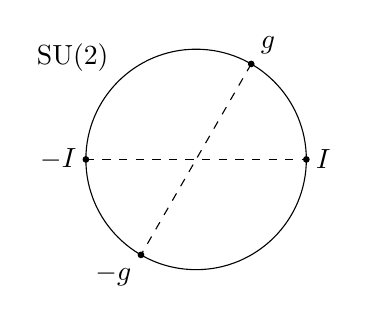
\begin{tikzpicture}[scale=0.7]
      \draw (0,0) circle (2);
      \draw[fill] (2,0) circle (0.05);
      \draw[fill] (-2,0) circle (0.05);
      \node[right] at (2,0) {$I$};
      \node[left] at (-2,0) {$-I$};
      \draw[fill] (1,1.732) circle (0.05);
      \draw[fill] (-1,-1.732) circle (0.05);
      \node[above right] at (1, 1.732) {$g$};
      \node[below left] at (-1, -1.732) {$-g$};
      \draw[dashed] (-2,0)--(2,0);
      \draw[dashed] (1, 1.732)--(-1, -1.732);
      \node[above left] at (-1.414, 1.414) {SU$(2)$};
    \end{tikzpicture}
  \end{center}

  We can in fact explicitly describe exponential map from $\mathfrak{so}(3)$ to SO$(3)$ with the following lemma. 

  \begin{lemma}[Rodrigues' Formula]
    The exponential map $exp: \mathfrak{so}(3) \rightarrow$ SO$(3)$ is defined by 
    \begin{equation}
      e^A = \cos{\theta} I_3 + \frac{\sin{\theta}}{\theta} A + \frac{(1 - \cos{\theta})}{\theta^2} B
    \end{equation}
    where 
    \begin{equation}
      A = \begin{pmatrix}
      0&-c&b\\c&0&-a\\-b&a&0
      \end{pmatrix}, B = \begin{pmatrix}
      a^2&ab&ac\\ab&b^2&bc\\ac&bc&c^2
      \end{pmatrix}
    \end{equation}
    This formula has many applications in kinematics, robotics, and motion interpolation. 
  \end{lemma}

  \begin{theorem}
  The Lie algebras for the following classical Lie groups are summarized as follows. 
  \begin{enumerate}
    \item $\mathfrak{sl}_n \mathbb{R}$ is the real vector space of real $n \times n$ matrices with null trace.
    \item $\mathfrak{so}(n)$ is the real vector space of real $n \times n$ skew-symmetric matrices. 
    \item $\mathfrak{gl}_n \mathbb{R}$ is the real vector space of all real $n \times n$ matrices.
    \item $\mathfrak{o}(n) = \mathfrak{o}(n)$
  \end{enumerate}
  \end{theorem}
  Note that the corresponding groups $\GL(n, \mathbb{R}), \SL(n, \mathbb{R}), \mathfrak{gl}_n \mathbb{R}, \mathfrak{sl}_n \mathbb{R}$ are Lie groups, meaning that they are smooth real manifolds. We can view each of them as smooth real manifolds embedded in the $n^2$ dimensional vector space of real matrices, which is isomorphic to $\mathbb{R}^{n^2}$. 

  \begin{theorem}
    The Lie algebras $\mathfrak{gl}_ \mathbb{R}, \mathfrak{sl}_n \mathbb{R}, \mathfrak{o}(n), \mathfrak{so}(n)$ are well-defined, but only 
    \begin{equation}
      exp: \mathfrak{so}(n) \rightarrow \text{SO}(n)
    \end{equation}
    is surjective. 
  \end{theorem}

  \begin{theorem}
    The Lie algebras for the following classical Lie groups are summarized as follows. 
    \begin{enumerate}
      \item $\mathfrak{sl}_2 \mathbb{C}$ is the real (or complex) vector space of traceless complex $n \times n$ matrices. 
      \item $\mathfrak{u}(n)$ is the real vector space of complex $n \times n$ skew-Hermitian matrices. 
      \item $\mathfrak{su}(n) = \mathfrak{u} \cap \mathfrak{sl}_2 \mathbb{C}$. It is also a real vector space. 
      \item $\mathfrak{gl}_n \mathbb{C}$ is the real (or complex) vector space of complex $n \times n$ matrices. 
    \end{enumerate}
    Note that even though the matrices in these Lie algebras have complex coefficients, we have assigned them to be in a \textbf{real} vector space, which means that we are only allowed to take real linear combinations of these elements. That is, the field we are working over is $\mathbb{R}$ (this does not contradict any of the axioms for vector spaces). For example an element $A$ in $\mathfrak{u}(n)$ or $\mathfrak{su}(n)$ must be anti-self adjoint, but $iA$ is self adjoint. 
  \end{theorem}

  Similarly, the Lie groups 
  \begin{equation}
    \GL(n, \mathbb{C}), \SL(n, \mathbb{C}), \mathfrak{gl}_n \mathbb{C}, \mathfrak{sl}_n \mathbb{C}
  \end{equation}
  are also smooth real manifolds embedded in Mat$(n, \mathbb{C}) \simeq \mathbb{C}^{n^2} \simeq \mathbb{R}^{2 n^2}$. So, we can view these four groups as manifolds embedded in $\mathbb{R}^{2 n^2}$. 

  Note some of the similarities and differences between the real and complex counterparts of these Lie groups and algebras. 
  \begin{enumerate}
    \item $\mathfrak{o}(n) = \mathfrak{so}(n)$, but $\mathfrak{u}(n) \neq \mathfrak{su}(n)$. 
    \item $exp: \mathfrak{gl}_n \mathbb{R} \rightarrow \GL(n, \mathbb{R})$ is not surjective, but $exp: \mathfrak{gl}_n \mathbb{C} \rightarrow \GL(n, \mathbb{C})$ is surjective due to the spectral theorem and surjectivity of $exp: \mathbb{C} \rightarrow \mathbb{C}^*$.
    \item The exponential maps $exp: \mathfrak{u}(n) \rightarrow \text{U}(n)$ and $exp: \mathfrak{su}(n) \rightarrow \text{SU}(n)$ are surjective. 
    \item Still, $exp: \mathfrak{sl}_2 \mathbb{C} \rightarrow \SL(2, \mathbb{C})$ is not surjective. This will be proved now. 
  \end{enumerate}

  \begin{theorem}
    $exp: \mathfrak{sl}_2 \mathbb{C} \rightarrow \SL(2, \mathbb{C})$ is not surjective. 
  \end{theorem}
  \begin{proof}
    Given $M \in \SL(n, \mathbb{C})$, assume that $M = e^A$ for some matrix $A \in \mathfrak{sl}_2 \mathbb{C}$. Putting $A$ into the Jordan Normal Form $J = N A N^{-1}$ means that $J$ can either be of form
    \begin{equation}
      J = \begin{pmatrix}
      0&1\\0&0
      \end{pmatrix}, \begin{pmatrix}
      \lambda&0\\0&-\lambda
      \end{pmatrix} \implies e^J = \begin{pmatrix}
      1&1\\0&1
      \end{pmatrix}, \begin{pmatrix}
      e^\lambda&0\\0&e^{-\lambda}
      \end{pmatrix}
    \end{equation}
    which is also in JNF in $\SL(2, \mathbb{C})$. But a matrix $P \in \SL(2, \mathbb{C})$ may exist with JNF of 
    \begin{equation}
      K = \begin{pmatrix}
      -1&1\\0&-1
      \end{pmatrix}
    \end{equation}
    which is not one of the 2 forms. So, $K \not\in \im{exp} \implies exp$ is not surjective. 
  \end{proof}

  \begin{theorem}
  The exponential maps 
  \begin{align*}
    & exp: \mathfrak{u}(n) \rightarrow \text{U}(n) \\
    & exp: \mathfrak{su}(n) \rightarrow \text{SU}(n)
  \end{align*}
  are surjective. 
  \end{theorem}

\subsubsection{Lie Algebra of SE(n)}

  Recall that the group of affine rigid isometries is denoted SE$(n)$. That is, 
  \begin{equation}
    \text{SE}(n) \equiv \text{SO}(n) \ltimes \text{Tran}\,\mathbb{R}^n
  \end{equation}
  We can define the matrix representation of this affine transformation as such. Given an element $g \in$ SE$(n)$ such that
  \begin{equation}
    g(x) \equiv R x + U, \; R \in \text{SO}(n), U \in \text{Tran}\, \mathbb{R}^n 
  \end{equation}
  we define the representation
  \begin{equation}
    \rho: \text{SE}(n) \rightarrow \GL(n+1, \mathbb{R}), \rho(g) \equiv \begin{pmatrix}
    R&U\\0&1
    \end{pmatrix}
  \end{equation}
  where $R$ is a real $n\times n$ matrix in SO$(n)$ and $U$ is a real $n$-vector in Tran$\,\mathbb{R}^n \simeq \mathbb{R}^n$. We would then have
  \begin{equation}
    \rho(g) \begin{pmatrix}
    x\\1
    \end{pmatrix} \equiv \begin{pmatrix}
    R&U\\0&1
    \end{pmatrix} \begin{pmatrix}
    x\\1
    \end{pmatrix} = \begin{pmatrix}
    R x + U\\1
    \end{pmatrix} \in \mathbb{R}^{n+1}
  \end{equation}

  Clearly, SE$(n)$ is a Lie group, and the matrix representation $\varrho$ of its Lie algebra $\mathfrak{se}(n)$ can be defined as the vector space of $(n+1) \times (n+1)$ matrices of the block form 
  \begin{equation}
    A = \begin{pmatrix}
    \Omega & U \\0 & 0
    \end{pmatrix}
  \end{equation}
  where $\Omega$ is an $n \times n$ skew-symmetric matrix and $U \in \mathbb{R}^n$. Note that there are two different exponential maps here: one belonging to the abstract Lie group SE$(n)$ and another belonging to the concrete, matrix group $\GL(n+1, \mathbb{R})$. This can be represented with the commutative diagram. 
  \[\begin{tikzcd}
  \mathfrak{se}(n) \arrow{r}{exp} \arrow{d}{\varrho} & SE(n) \arrow{d} {\rho}\\
  \mathfrak{gl}_{n+1} \mathbb{R} \arrow{r}{exp} & \GL(n+1, \mathbb{R})
  \end{tikzcd}\]

  \begin{lemma}
    Given any $(n+1) \times (n+1)$ matrix of form 
    \begin{equation}
      A = \begin{pmatrix}
       \Omega & U \\0&0
      \end{pmatrix}
    \end{equation}
    where $\Omega$ is any matrix and $U \in \mathbb{R}^n$, 
    \begin{equation}
      A^k = \begin{pmatrix}
      \Omega^k & \Omega^{k-1} U \\0&0
      \end{pmatrix}
    \end{equation}
    where $\Omega^0 = I_n$, which implies that
    \begin{equation}
      e^A = \begin{pmatrix}
      e^\Omega & V U \\ 0 & 1
      \end{pmatrix}, \; V = I_n + \sum_{k \geq 1} \frac{\Omega^k}{(k+1)!}
    \end{equation}
  \end{lemma}

  \begin{theorem}
    The exponential map
    \begin{equation}
      exp: \mathfrak{se}(n) \rightarrow SE(n)
    \end{equation}
    is well-defined and surjective. 
  \end{theorem}

\subsection{Representations of Lie Groups and Lie Algebras}

  Let $\mathcal{G}$ be an abstract group and let
  \begin{equation}
    \rho: \mathcal{G} \rightarrow \GL(V)
  \end{equation}
  be the representation of $\mathcal{G}$. Then, let $\mathfrak{g}$ be the Lie algebra of $\mathcal{G}$, and $\mathfrak{gl}(V)$ be the Lie algebra of $\GL(V)$. Then, $\rho$ induces another homomorphism 
  \begin{equation}
    \varrho: \mathfrak{g} \rightarrow \mathfrak{gl}(V)
  \end{equation}
  where the bracket structure (in this case, the comutator in the matrix algebra) is preserved. 
  \begin{equation}
    \varrho([X,Y]) = [\varrho(X), \varrho(Y)]
  \end{equation}
  We can visualize this induced homomorphism with the following commutative diagram, which states that $\rho \circ exp = exp \circ \varrho$. 

  \[\begin{tikzcd}
  \mathcal{G} \arrow{r}{\rho} & \GL(V)\\
  \mathfrak{g} \arrow{u}{exp} \arrow{r}{\varrho} & \mathfrak{gl}(V) \arrow{u}{exp}
  \end{tikzcd}\]

  Note that there are very crucial differences between $\rho$ and $\varrho$. First, $\rho$ is a homomorphism between \textbf{groups}, while $\varrho$ is a homomorphism between \textbf{vector spaces}. Additionally, $\GL(V)$ is a group, not a linear space, while $\mathfrak{gl}(V)$ is a linear space. Finally, note that $\GL(V)$ is restricted to only matrices with nonzero determinants, while the elements of $\mathfrak{gl}(V)$ can be any matrix. 

  \begin{example}
    The representation of SE$(n)$ to $\GL(n+1 \mathbb{R}$ and $\mathfrak{se}(n)$ to $\mathfrak{gl}_{n+1} \mathbb{R}$ induces the second homomorphism $\varrho: \mathfrak{gl}_{n+1} \mathbb{R} \rightarrow \GL(n+1, \mathbb{R})$. 
  \end{example}

  \begin{definition}
    The direct sum of representations is a representation. That is, if $U$ is a representation and $V$ is a representation, then $U \oplus V$ is a representation. That is, if 
    \begin{equation}
      \rho_1: \mathcal{G} \rightarrow U, \; \rho_1 (g) = \begin{pmatrix}
      u_1&u_2\\u_3&u_4
      \end{pmatrix}
    \end{equation}
    and
    \begin{equation}
      \rho_2: \mathcal{G} \rightarrow V, \; \rho_2 (g) = \begin{pmatrix}
      v_1 & v_2 \\ v_3 & v_4
      \end{pmatrix}
    \end{equation}
    are two representations of the same group element $g \in \mathcal{G}$, then 
    \begin{equation}
      (\rho_1 \oplus \rho_2): \mathcal{G} \rightarrow (U \oplus V), \;(\rho_1 \oplus \rho_2) (g) = \begin{pmatrix}
      u_1 & u_2 & 0 & 0 \\
      u_3 & u_4 & 0 & 0 \\
      0 & 0 & v_1 & v_2 \\
      0 & 0 & v_3 & v_4 
      \end{pmatrix}
    \end{equation}
    is a bigger representation of $g$ in $U \oplus V$. 
  \end{definition}

  \begin{definition}
    $V$ is irreducible if the only subspaces which are representations are only $V$ and $\{0\}$. 
  \end{definition}

  For our case, we will consider that any representation can be written as a direct sum of irreducible representations. We will now proceed to find an irreducible representation of $\mathfrak{sl}_2 \mathbb{C}$. This means that we want to find the smallest (lowest dimensional) vector space $V$ such that there exists a representation
  \begin{equation}
    \varrho: \mathfrak{sl}_2 \mathbb{C} \rightarrow \mathfrak{gl}(V)
  \end{equation}
  We will write, as shorthand notation, that 
  \begin{equation}
    H = \varrho(H), X = \varrho(X), Y = \varrho(Y)
  \end{equation}
  Clearly, $H, X, Y \in \mathfrak{gl}(V) \simeq \mathfrak{gl}(\mathbb{C}^n)$. By the spectral theorem, we can find an orthonormal basis of eigenvectors $e_1, e_2, ..., e_n$ of the mapping $H$ such that
  \begin{equation}
    H e_i = \lambda_i e_i, \; \lambda_i \in \mathbb{C}
  \end{equation}
  Since $[H,X] = 2X$, it follows that $HX e_i - X H e_i = 2X e_i \implies H (X e_i) = (\lambda_i + 2) (X e_i) \implies Xe_i$ for all $i = 1, 2, ..., n$ are also eigenvectors of $H$ with eigenvalue $(\lambda_i + 2)$, or $X e_i = 0$. So, $X$ is a "ladder operator" that maps each eigenvector $e_i$ with eigenvalue $\lambda_i$ to a different eigenvector $e_j$ with eigenvalue $\lambda_j = \lambda_i + 2$. Having nowhere to be mapped to, the eigenvector with the largest eigenvalue (which must exist since $V$ is finite dimensional) will get mapped to the $0$ vector by $X$. Let us denote this eigenvector having the maximum eigenvalue $m$, as $v_m$. 

  Similarly, $[H,Y] = -2Y$ implies that
  \begin{equation}
    HY e_i - YH e_i = -2Y e_i \implies H(Y e_i) = (\lambda_i - 2)(Y e_i)
  \end{equation}

  implying that $Y$ maps each eigenvector $e_i$ with eigenvaue $\lambda_i$ to another eigenvector $e_j$ with eigenvalue $\lambda_j = \lambda_i - 2$, except for the eigenvector with smallest eigenvalue, which gets mapped to $0$. Since $Y$ clearly maps each eigenvector to a different eigenvector that has a strictly decreasing eigenvalue, we can construct a basis of $V$ to be
  \begin{equation}
    \{v_m, Y v_m, Y^2 v_m, Y^3 v_m, ..., Y^{n-1} v_m\}
  \end{equation}
  (remember that $Y^n v_m = 0$). So, elements of $\mathfrak{sl}_2 \mathbb{C}$ acts on the space $V$ with basis above. To continue, we introduce the following theorem. 

  \begin{theorem}
    \begin{equation}
      X Y^j v_m = j(m-j+1) Y^{j-1} v_m
    \end{equation}
  \end{theorem}
  \begin{proof}
    By induction on $j$ using bracket relations.
  \end{proof}

  $V$ is $n$-dimensional. Since $Y^n v_m = 0$ and $Y^{n-1} v_m \neq 0$, we use the theorem above to get
  \begin{equation}
    0 = X Y^n v_m = n (m-n+1) Y^{n-1} v_m \implies m-n+1=0
  \end{equation}
  So, $n = m+1$, which means that the eigenvalues of $H$ are
  \begin{equation}
    m, m-2, m-4, \ldots, m - 2(n-1) = -m
  \end{equation}

  and we are done. We now classify the 1, 2, and 3 dimensional irreducible representations of $\mathfrak{sl}_2 \mathbb{C}$. 
  \begin{enumerate}
    \item When $n = 1$ (i.e. dimension is 1), $m = n-1 = 0$, meaning that the greatest (and only) eigenvalue is $0$. That is, 
      \begin{equation}
        H v_0 = 0,\; X v_0 = 0,\; Y v_0 = 0
      \end{equation}
    which is the trivial representation of $\mathfrak{sl}_2 \mathbb{C}$. Explicitly, we can completely define the representation (which is a linear homomorphism) with the three equations. 
    \begin{equation}
      \varrho(H) = (0),\; \varrho(X) = (0),\; \varrho(Y) = (0)
    \end{equation}

    \item When $n = 2$ and $m=1$. We now look for a 2 dimensional irreducible representation. The eigenvalues are $1$ and $-1$, with $\{v_1, v_{-1}\}$ as a basis of 2 dimensional space $V$. Then we have 
      \begin{align*}
        & Hv_1 = v_1, \; Hv_{-1} = - v_{-1} \\
        & X v_1 = 0, \; X v_{-1} = v_1 \\
        & Y v_1 = v_{-1}, \; Y v_{-1} = 0
      \end{align*}
    which explicitly translates to the representation $\varrho$ being defined
    \begin{equation}
      \varrho(H) = \begin{pmatrix}
      1&0\\0&-1
      \end{pmatrix}, \; \begin{pmatrix}
      0&1\\0&0
      \end{pmatrix}, \; \begin{pmatrix}
      0&0\\1&0
      \end{pmatrix}
    \end{equation}

    \item When $n=3 \implies m=2$, the basis is $\{v_{-2}, v_0, v_2\}$ with eigenvalues $2, 0, -2$, and the irreducible representation $\varrho$ is defined
      \begin{equation}
        \varrho(H) = \begin{pmatrix}
        2&&\\&0&\\&&-2
        \end{pmatrix}, \varrho(Y) = \begin{pmatrix}
        0&0&0\\1&0&0\\0&1&0
        \end{pmatrix}, \varrho(X) = \begin{pmatrix}
        0&1&0\\0&0&1\\0&0&0
        \end{pmatrix}
      \end{equation}

    \item The same process continues on for $n=4, 5, ...$, and this entirely classifies the irreducible representations of $\mathfrak{sl}_2 \mathbb{C}$. 
  \end{enumerate} 

  \pagebreak

  \subsubsection{Tensor Products of Group Representations}

    \begin{definition}
      If $V$ and $W$ are two different representations of a group $\mathcal{G}$, then we know that $V \oplus W$ is also a representation of $\mathcal{G}$. Furthermore, the tensor product space $V \otimes W$ also defines a representation of $\mathcal{G}$. That is, given representations
      \begin{align*}
        & \rho_V: \mathcal{G} \rightarrow \GL(V) \\
        & \rho_W: \mathcal{G} \rightarrow \GL(W)
      \end{align*}
      The homomorphism $\rho_V \otimes \rho_W: \mathcal{G} \rightarrow \GL(V \otimes W)$ is also a representation of $\mathcal{G}$, which is defined
      \begin{equation}
        (\rho_V \otimes \rho_W)(g) (v \otimes w) \equiv \rho_V (g) (v) \otimes \rho_W (g) (w)
      \end{equation}
      or represented in shorthand notation, 
      \begin{equation}
        g(v \otimes w) \equiv (g v) \otimes (g w)
      \end{equation}
      We know that exp$(H)$ acts on $V$ and $W$ since it is an element of $\GL(V)$ and $\GL(W)$. This means that
      \begin{equation}
        exp(H)(v \otimes w) \equiv \big( exp(H)(v)\big) \otimes \big( exp(H)(w)\big)
      \end{equation}
      If $H$ ($= \rho_V (H)$ or $\rho_W(H)$) has an eigenvalue $\lambda$ on $v$ in $V$ and eigenvalue $\mu$ on $w$ in $W$, then 
      \begin{equation}
        exp(H) (v \otimes w) = (e^\lambda v) \otimes (e^\mu w) = e^{\lambda + \mu} v \otimes w
      \end{equation}
      That is, eigenvalues of $H$ \textbf{add} on tensor products. 
    \end{definition}

    \begin{example}
      Recall that the $2$ dimensional representation $V$ of $\mathfrak{sl}_2 \mathbb{C}$ has eigenvalues $1$ and $-1$ (with corresponding eigenvectors $e_1$ and $e_{-1}$). So, $V \otimes V$ has eigenvalues 
      \begin{align*}
        & (-1) + (-1) = -2, \;\; (-1) + 1 = 0 \\
        & 1 + (-1) = 0, \;\; 1 + 1 = 2
      \end{align*}
      Therefore, the eigenvalues of $V \otimes V$ is $-2$ (geometric multiplicity of 1), $0$ (geometric multiplicity of 2), and $2$ (geometric multiplicity of 1), (Notation-wise, the $n$-dimensional irreducible representation of $\mathfrak{sl}_2 \mathbb{C}$ is denoted $\mathbf{n}$.) which means that
      \begin{equation}
        \mathbf{2} \otimes \mathbf{2} = \mathbf{3} \oplus \mathbf{1}
      \end{equation}
      We can decompose $V \otimes V$ into its symmetric and exterior power components. Sym$^2 V$ has basis (of eigenvectors)
      \begin{equation}
        \{e_{-1} \odot e_{-1}, \; e_{-1} \odot e_1, \; e_1 \odot e_1\}
      \end{equation}
      where the corresponding eigenvalues are $-2$, $0$, and $2$, respectively. So, $\dim{Sym^2 V} = 3$, which means that $Sym^2 V = \mathbf{3}$. As for the exterior power component of $V$, $\Lambda^2 V$ has basis $\{e_{-1} \wedge e_1\}$ with eigenvalue $= 0 \implies \dim{\Lambda^2 V} = 1$, meaning that $\Lambda^2 V = \mathbf{1}$. Therefore, 
      \begin{equation}
        V \otimes V = Sym^2 V \oplus \Lambda^2 V = \mathbf{3} \oplus \mathbf{1}
      \end{equation}
    \end{example}

\subsection{Topological Decompositions of Lie Groups}

  \begin{definition}
    Let us define 
    \begin{enumerate}
      \item S$(n)$ is the vector space of real, symmetric $n \times n$ matrices. 
      \item SP$(n)$ is the set of symmetric, positive semidefinite matrices. 
      \item SPD$(n)$ is the set of symmetric, positive definite matrices. 
    \end{enumerate}
    Note that SP$(n)$ and SPD$(n)$ are not even vector spaces at all. 
  \end{definition}

  \begin{lemma}
    The exponential map 
    \begin{equation}
      exp: S(n) \rightarrow SPD(n)
    \end{equation}
    is a homeomorphism. One may be tempted to call S$(n)$ the Lie algebra of SPD$(n)$, but this is not the case. S$(n)$ is not even a Lie algebra since the commutator is not algebraically closed. Furthermore, SPD$(n)$ is not even a multiplicative group (since matrix multiplication is not closed). 
  \end{lemma}

  Recall from linear algebra the Polar Decomposition. We express this result in a slightly modified way. 

  \begin{theorem}[Polar Decomposition]
    Given a Euclidean space $\mathbb{E}^n$ and any linear endomorphism $f$ of $\mathbb{E}^n$, there are two positive definite self-adjoint linear maps $h_1, h_2 \in$ End$(\mathbb{E}^n)$ and $g \in$ O$(n)$ such that
    \begin{equation}
      f = g \circ h_1 = h_2 \circ g
    \end{equation}
    That is, such that $f$ can be decomposed into the following compositions of functions that commute. 

    \[\begin{tikzcd}
    \mathbb{E}^n \arrow{r}{h_2} & \mathbb{E}^n \\
    \mathbb{E}^n \arrow{u}{g} \arrow{ur}{f} \arrow{r}{h_1} & \mathbb{E}^n \arrow{u}{g}
    \end{tikzcd}\]

    This means that there is a bijection between $Mat(n, \mathbb{R})$ and $O(n) \times SP(n)$. If $f$ is an automorphism, then this decomposition is unique. 
  \end{theorem}

  \begin{corollary}
    The two topological groups are homeomorphic. 
    \begin{equation}
      GL(n, \mathbb{R}) \cong O(n) \times SPD(n)
    \end{equation}
  \end{corollary}

  \begin{corollary}
    For every invertible real matrix $A \in GL(n, \mathbb{R})$, there exists a unique orthogonal matrix $R$ and unique symmetric matrix $S$ such that
    \begin{equation}
      A = R e^S
    \end{equation}
    $\implies$ there is a bijection between $\GL(n, \mathbb{R})$ and $O(n) \times S(n) \simeq \mathbb{R}^{n(n+1)/2}$. Moreover, they are homeomorphic. That is, 
    \begin{equation}
      \GL(n, \mathbb{R}) \simeq O(n) \times S(n) \simeq O(n) \times \mathbb{R}^{n(n+1)/2}
    \end{equation}
    This essentially reduces the study of $\GL(n, \mathbb{R})$ to the study of $O(n)$, which is nice since $O(n)$ is compact. 
  \end{corollary}

  \begin{corollary}
    Given a real matrix $A$, if $\det{A} > 0$, then we can decompose $A$ as
    \begin{equation}
      A = R e^S
    \end{equation}
    where $R \in SO(n)$ and $S \in S(n)$. 
  \end{corollary}

  \begin{corollary}
    There exists a bijection between
    \begin{equation}
      \SL(n, \mathbb{R}) \text{ and } SO(n) \times (S(n) \cap \mathfrak{sl}_n \mathbb{R})
    \end{equation}
  \end{corollary}
  \begin{proof}
    $A \in \SL(n, \mathbb{R}) \implies 1 = \det{A} = \det{R} \det{e^S} = \det{e^S} \implies \det{e^S} = e^{\Tr{S}} = 1 \implies \Tr{S} = 0 \implies S \in$ S$(n) \cap \mathfrak{sl}_n \mathbb{R}$. 
  \end{proof}

  \begin{definition}
    Let us define
    \begin{enumerate}
      \item H$(n)$ is the real vector space of $n \times n$ Hermitian matrices. 
      \item HP$(n)$ is the set of Hermitian, positive semidefinite $n \times n$ matrices. 
      \item HPD$(n)$ is the set of Hermitian, positive definite $n \times n$ matrices. 
    \end{enumerate}
    Similarly, HP$(n)$ and HPD$(n)$ are not vector space. They are just sets. 
  \end{definition}

  \begin{lemma}
    The exponential mapping
    \begin{equation}
      exp: H(n) \rightarrow HPD(n)
    \end{equation}
    is a homeomorphism. 
  \end{lemma}

  However again, HPD$(n)$ is not a Lie group (multiplication is not algebraically closed) nor is H$(n)$ a Lie algebra (commutator is not algebraically closed). By the polar form theorem of complex $n \times n$ matrices, we have a (not necessarily unique) bijection between
  \begin{equation}
    \text{Mat}(n, \mathbb{C}) \text{ and } U(n) \times HP(n)
  \end{equation}
  which implies that
  \begin{equation}
    \GL(n, \mathbb{C}) \cong U(n) \times HPD (n)
  \end{equation}

  \begin{corollary}
    For every complex invertible matrix $A$, there exists a unique decomposition
    \begin{equation}
      A = U e^S
    \end{equation}
    where $U \in U(n)$ and $S \in H(n)$, which implies that the following groups are homeomorphic. 
    \begin{align*}
      \GL(n, \mathbb{C}) & \cong U(n) \times H(n) \\
      & \cong U(n) \times \mathbb{R}^{n^2}
    \end{align*} 
    This essentially reduces the study of $\GL(n, \mathbb{C})$ to that of U$(n)$. 
  \end{corollary}

  \begin{corollary}
    There exists a bijection between 
    \begin{equation}
      \SL(n, \mathbb{C}) \text{ and } SU(n) \times (H(n) \cap \mathfrak{sl}_n \mathbb{C})
    \end{equation}
  \end{corollary}
  \begin{proof}
    Similarly, when $A = U e^S$, we know that $|\det{U}| = 1$ and $\Tr{S}$ is real (since by the Spectral theorem, every self adjoint matrix has a real spectral decomposition). Since $S$ is Hermitian, this implies that $\det{e^S} > 0$. If $A \in \SL(n, \mathbb{C})$, then $\det{A} = 1 \implies \det{e^S} = 1 \implies S \in H(n) \cap \mathfrak{sl}_n \mathbb{C}$. 
  \end{proof}

\subsection{Linear Lie Groups}

  We will assume that the reader has the necessary background knowledge in manifolds, chart mappings, diffeomorphisms, tangent spaces, and transition mappings. 

  Recall that the algebra of real $n \times n$ matrices Mat$(n, \mathbb{R})$ is bijective to $\mathbb{R}^{n^2}$, which is a topological space. Therefore, this bijection 
  \begin{equation}
    i:(\mathbb{R}^{n^2}, \tau_E) \rightarrow \text{Mat}(n, \mathbb{R})
  \end{equation}
  induces a topology on Mat$(n, \mathbb{R})$, defined 
  \begin{equation}
    \tau_M \equiv \{U \in \text{Mat}(n, \mathbb{R}) \; | \; e^{-1} (U) \in \tau_E\}
  \end{equation}
  With this, consider the subset
  \begin{equation}
    \GL(n, \mathbb{R}) \subset \text{Mat}(n, \mathbb{R})
  \end{equation}
  where
  \begin{equation}
    \GL(n, \mathbb{R}) \equiv \{x \in \text{Mat}(n, \mathbb{R}) \;|\; \det{x} \neq 0\}
  \end{equation}
  This set, as we expect, is a multiplicative group. 

  \begin{definition}
    The \textbf{general linear group}, denoted $\GL(n, \mathbb{R})$ is the set of $n \times n$ matrices with nonzero determinant. The more technical definition is that $\GL(n, \mathbb{R})$ is really just the automorphism group of $\mathbb{R}^n$, 
    \begin{equation}
      \GL(n, \mathbb{R}) \equiv \text{Aut}(\mathbb{R}^n)
    \end{equation}
    but it is customary to assume a basis on $\mathbb{R}^n$ in order to realize $\GL(n, \mathbb{R})$ as a matrix group. Note that the procedure of assuming a basis on $\mathbb{R}^n$ is the same as defining a representation of the abstract group $\GL(n, \mathbb{R})$. Both assigns a real $n \times n$ matrix to each element of $\GL(n, \mathbb{R})$. 
  \end{definition}

  In this way, we can view $\GL(n, \mathbb{R})$ as a topological space in $\mathbb{R}^{n^2}$, and it is fine to interpret $\GL(n, \mathbb{R})$ as a matrix group rather than an abstract group. 

  Since the matrix representation of $\GL(n, \mathbb{R})$ is always well defined, the abstract subgroups of $\GL(n, \mathbb{R})$, which are $\SL(n, \mathbb{R}), O(n)$, and $SO(n)$, also have well defined matrix representations (that we are all familiar with). Additionally, since there exists a bijection
  \begin{equation}
    \text{Mat}(n, \mathbb{C}) \cong \mathbb{C}^{n^2} \cong \mathbb{R}^{2 n^2}
  \end{equation}
  we can view $\GL(n, \mathbb{C})$ as a subset of $\mathbb{R}^{2n^2}$, meaning that the subgroups $\SL(n, \mathbb{C}), U(n)$, and $SU(n)$ of $\GL(n, \mathbb{C})$ can also be viewed as subsets of $\mathbb{R}^{2n^2}$. This also applies to $SE(n)$ since it is a subgroup of $\SL(n+1, \mathbb{R})$. We formally state it now. 

  \begin{theorem}
    SE$(n)$ is a linear Lie group. 
  \end{theorem}
  \begin{proof}
    The matrix representation of elements $g \in SE(n)$ is 
    \begin{equation}
      \rho(g) \equiv \begin{pmatrix}
      R_g & U_g \\ 0 & 1
      \end{pmatrix}, \; R_g \in SO(n), U_g \in \mathbb{R}^n
    \end{equation}
    But such matrices also belong to the bigger group $\SL(n+1, \mathbb{R}) \implies SE(n) \subset \SL(n+1, \mathbb{R})$. Moreover, this canonical embedding 
    \begin{equation}
      i: SE(n) \rightarrow \SL(n+1, \mathbb{R})
    \end{equation}
    is a group homomorphism since
    \begin{align*}
      i\big( \rho(g_1 \cdot g_2) \big) & = \begin{pmatrix}
      RS & RV + U \\ 0 & 1
      \end{pmatrix} \\
      & = \begin{pmatrix}
      R & U \\ 0 & 1
      \end{pmatrix} \begin{pmatrix}
      S & V \\ 0 & 1
      \end{pmatrix} = \rho \big( i(g_1) \cdot i(g_2) \big) 
    \end{align*}
    and the inverse is given by 
    \begin{equation}
      \begin{pmatrix}
      R & U \\ 0 & 1
      \end{pmatrix}^{-1} = \begin{pmatrix}
      R^{-1} & - R^{-1} U \\ 0 & 1
      \end{pmatrix} = \begin{pmatrix}
      R^T & - R^T U \\ 0 & 1
      \end{pmatrix}
    \end{equation}
    is also consistent between the inverse operation in SE$(n)$ and $\SL(n+1, \mathbb{R})$. Therefore, SE$(n)$ is a subgroup of $\SL(n+1, \mathbb{R})$, which is a subgroup of $\GL(n+1, \mathbb{R})$. 
  \end{proof}

  Note that even though SE$(n)$ is diffeomorphic (a topological relation) to SO$(n) \times \mathbb{R}^n$, it is \textbf{not} isomorphic (an algebraic relation) sicne group operations are not preserved. Therefore, we write this "equality" as a semidirect product of groups. 
  \begin{equation}
    SE(n) \equiv SO(n) \ltimes \mathbb{R}^n
  \end{equation}

  Therefore, all of the classical Lie groups that we have mentioned can be viewed as subsets of $\mathbb{R}^N$ (with the subspace topology) and as subgroups of $\GL(N, \mathbb{R})$ for some big enough $N$. This defines a special family of Lie groups, called linear Lie groups. 

  \begin{definition}
    A \textbf{linear Lie group} is a subgroup of $\GL(n, \mathbb{R})$ for some $n \geq 1$ which is also a smooth manifold in $\mathbb{R}^{n^2}$. 
  \end{definition}

  \begin{theorem}[Von Neumann, Cartan]
    A closed subgroup $\mathcal{G}$ of $\GL(n, \mathbb{R})$ is a linear Lie group. That is, a closed subgroup $\mathcal{G}$ of $\GL(n, \mathbb{R})$ is a smooth manifold in $\mathbb{R}^{n^2}$.
  \end{theorem}

  \begin{definition}
    Since a linear Lie group $\mathcal{G}$ is a smooth submanifold in $\mathbb{R}^N$, we can take its tangent space at the identity element $I$, which is defined 
    \begin{equation}
      T_I \mathcal{G} \equiv \{p^\prime (0) \;|\; p: I \subset \mathbb{R} \rightarrow \mathcal{G}, p(0) = I\}
    \end{equation}
    where $p$ is a path function on $\mathcal{G}$. 
  \end{definition}

  Note that we haven't mentioned anything about the exponential map up to now. We mention the relationship between this map and the Lie algebra with the following theorem. 

  \begin{theorem}
    Let $\mathcal{G}$ be a linear Lie group. The set $\mathfrak{g}$ defined such that
    \begin{equation}
      \mathfrak{g} \equiv \{X \in \text{Mat}(n, \mathbb{R}) \; | \; e^{t X} \in \mathcal{G} \; \forall t \in \mathbb{R}\}
    \end{equation}
    is equal to the tangent space of $\mathcal{G}$ at the identity element. That is, 
    \begin{equation}
      \mathfrak{g} = T_I \mathcal{G}
    \end{equation}
    Furthermore, $\mathfrak{g}$ is closed under the commutator 
    \begin{equation}
      [A,B] \equiv A B - B A
    \end{equation}
  \end{theorem}

  This theorem ensures that given a linear Lie group $\mathcal{G}$, the tangent space $\mathfrak{g}$ exists and is closed under the commutator. We formally define this space. 

  \begin{definition}
    The Lie algebra of a linear Lie group is a real vector space (of matrices) together with a algebraically closed bilinear map 
    \begin{equation}
      [A,B] \equiv A B - B A
    \end{equation}
    called the \textbf{commutator}. 
  \end{definition} 

  The definition of $\mathfrak{g}$ given in the previous theorem shows that 
  \begin{equation}
    exp: \mathfrak{g} \rightarrow \mathcal{G}
  \end{equation}
  is well defined. In general, exp is neither injective nor surjective. Visually, this exponential mapping is what connects the Lie algebra, i.e. the tangent space of manifold $\mathcal{G}$ to the actual Lie group $\mathcal{G}$. To define the inverse map that maps Lie group elements to Lie algebra ones, we can simply just compute the tangent vectors of the manifold $\mathcal{G}$ at the identity $I$ by taking the derivative of arbitrary path functions in $\mathcal{G}$. That is, for every $X \in T_I \mathcal{G}$, we define the smooth curve 
  \begin{equation}
    \gamma_X: t \mapsto e^{tX}
  \end{equation}
  where $\gamma_X(0) = I$. If we take the derivative of this curve, with respect to $t$ at $t = 0$, we will get the tangent vector $X$ corresponding to that group element $g = e^{X}$. More visually, we just need to take the collection of all smooth path functions $\gamma$ on manifold $\mathcal{G}$ such that $\gamma(0) = I$. Then, taking the derivative of all these paths at $t = 0$ will produce the collection of all tangent vectors at the identity element. We show this process in the following examples. 

  \begin{theorem}
    The matrix representation of $\mathfrak{sl}_n \mathbb{R}$ is precisely the set of traceless $n \times n$ matrices. 
  \end{theorem}

  \begin{proof}
    Clearly, $\mathfrak{sl}_n \mathbb{R}$ is a vector space since it is a Lie algebra. So, $X \in \mathfrak{sl}_n \mathbb{R} \implies t X \in \mathfrak{sl}_n \mathbb{R}$ for all $t \in \mathbb{R} \implies \det{e^{tX}} = 1$ for all $t \in \mathbb{R}$, for all $X \in \mathfrak{sl}_n \mathbb{R}$. But we use the identity 
    \begin{align*}
      \det{e^{tX}} = e^{\Tr{(tX)}} & \implies 1 = e^{\Tr{(t X)}} \\
      & \implies \Tr{(tX)} = 0 \\
      & \implies \Tr{(X)} t = 0 \implies \Tr{X} = 0
    \end{align*}
  \end{proof}
  We now provide an alternative, better proof. We first need a lemma. 

  \begin{lemma}
    $\det^\prime (I) = \Tr$. That is, the differential of the $\det$ operator, evaluated at the identity matrix, is equal to the trace. That is, given any matrix $T$ in the vector space of matrices, 
  \end{lemma}
  \begin{proof}
    \begin{align*}
      \det^\prime (I) (T) = \nabla_T \det(I) \\
      & = \lim_{\varepsilon \rightarrow 0} \frac{\det{(I + \varepsilon T)} - \det{I}}{\varepsilon} \\
      & = \lim_{\varepsilon \rightarrow 0} \frac{\det{(I + \varepsilon T)} - 1}{\varepsilon}
    \end{align*}
    Clearly, $\det(I + \varepsilon(T)) \in \mathbb{R}[\varepsilon]$, where the constant term of the polynomial approaches $1$ and the linear term (coefficient of $\varepsilon$) is $\Tr{T}$. So, 
    \begin{equation}
      \nabla_T \det{I} = \lim_{\varepsilon \rightarrow 0} ... + \Tr{T} = \Tr{T}
    \end{equation}
  \end{proof}

  This means that the instantaneous rate at which $\det$ changes at $I$ when traveling in direction $T$ is directly proportional to $\Tr{T}$. Now, we provide an alternative proof of the theorem. 
  \begin{proof}
    Let $R: \mathbb{R} \rightarrow \SL(n, \mathbb{R})$ such that $R(0) = I$. Then, by definition, $\im{R} \subset \SL(n, \mathbb{R}) \implies \det{(R(t))} = 1$ for all $t \in (-\varepsilon, \varepsilon)$. Compute the derivative of the mapping $\det \circ R$. 
    \begin{align*}
        (\det \circ  R) (t) = 1 & \implies \det^\prime \big( R(t) \big) \cdot R^\prime (t) \\ 
        & \implies \det^\prime (I) = \det^\prime \big(R(t)\big) = 0 
    \end{align*}
    We now use the previous lemma get that 
    \begin{equation}
      \det^\prime \big( R^\prime(0)\big) = \det^\prime (I)=0 \implies \Tr{R^\prime(0)} = 0
    \end{equation}
  \end{proof} 

  \begin{theorem}
    The matrix representation of $\mathfrak{so}(n)$ is precisely the set of antisymmetric matrices. 
  \end{theorem}
  \begin{proof}
    Let $R: \mathbb{R} \rightarrow SO(n)$ be a arbitrary smooth curve in $\SL(n)$ such that $R(0) = I$. Then, for all $t \in (-\epsilon, \epsilon)$, 
    \begin{equation}
      R(t) R(t)^T = I
    \end{equation}
    Taking the derivative at $t = 0$, we get
    \begin{equation}
      R^\prime (0) R(0)^T + R(0) R^\prime(0)^T = 0 \implies R^\prime (0) + R^\prime(0)^T = 0
    \end{equation}
    which states that the tangent vector $X = R^\prime (0)$ is skew symmetric. Since the diagonal elements of a skew symmetric matrix are $0$, the trace is $0$ and the condition that $\det{R} = 1$ yields nothing new. This shows that $\mathfrak{o}(n) = \mathfrak{so}(n)$. 
  \end{proof}




  We have only worked with linear Lie groups so far. The reason that linear Lie groups are so nice to work with is because they have well defined matrix representations. This allows us to have concrete structures on these groups and their Lie algebras. 
  \begin{enumerate}
    \item A linear Lie group is concretely defined as a submanifold of $\mathbb{R}^N$, while a general one is an abstract manifold. 
    \item The Lie bracket with regards to a linear Lie group is defined to be the commutator 
      \begin{equation}
        [A,B] \equiv A B - B A
      \end{equation}
    but for elements that are not matrices this doesn't make sense. 

    \item The exponential map from the algebra to the group is defined
      \begin{equation}
        e^A \equiv \sum_{k=0}^\infty \frac{1}{k!} A^k
      \end{equation}
    but if $A$ is not a matrix, then exp cannot be defined this way.
  \end{enumerate}
  We seek to generalize these concepts to abstract Lie groups, but we will do this in the next section. 

  \subsubsection{Lie Algebras of SO(3) and SU(2), Revisited}

    \begin{example}
      The Lie algebra $\mathfrak{so}(3)$ is the real vector space of $3 \times 3$ skew symmetric matrices of form 
      \begin{equation}
        \begin{pmatrix}
        0 & -d & c \\ d & 0 & -b \\ -c & b & 0
        \end{pmatrix}
      \end{equation}
      where $b, c, d \in \mathbb{R}$. The Lie bracket $[A,B]$ of $\mathfrak{so}(3)$ is also just the usual commutator. 

      We can define an isomorphism of Lie algebras $\psi: (\mathbb{R}^3, \times) \rightarrow \mathfrak{so}(3)$ (where $\times$ is the cross product) by the formula 
      \begin{equation}
        \psi(b, c, d) \equiv \begin{pmatrix}
        0 & -d & c \\
        d & 0 & -b \\
        -c & b & 0
        \end{pmatrix}
      \end{equation}
      where, by definition, 
      \begin{equation}
        \psi(u \times v) = [\psi(u), \psi(v)]
      \end{equation}
      It is also easily verified that for all $u, v \in \mathbb{R}^3$, 
      \begin{equation}
        \psi(u) (v) = u \times v
      \end{equation}
    \end{example}

    \begin{example}
      Similarly, we can see that $\mathfrak{su}(2)$ is the real vector space consisting of all complex $2 \times 2$ skew Hermitian matrices of null trace, which is of form
      \begin{equation}
        i(d \sigma_1 + c \sigma_2 + b \sigma_3) = \begin{pmatrix}
        i b & c + i d\\
        -c + i d & - i b
        \end{pmatrix}
      \end{equation}
      where $\sigma_1, \sigma_2, \sigma_3$ are the Pauli spin matrices. We can also define an isomorphism of Lie algebras $\varphi: (\mathbb{R}^3, \times) \rightarrow \mathfrak{su}(2)$ by the formula
      \begin{equation}
        \varphi(b, c, d) = \frac{i}{2} (d \sigma_1 + c \sigma_2 + b \sigma_3) = \frac{1}{2} \begin{pmatrix}
        i b & c + i d\\
        -c + i d & - i b
        \end{pmatrix}
      \end{equation}
      where, by definition of ismorphism, we have
      \begin{equation}
        \varphi(u \times v) = [\varphi(u), \varphi(v)]
      \end{equation}
    \end{example}

    We now restate the connection between the groups SO$(3)$ and SU$(2)$. Note that letting $\theta = \sqrt{b^2 + c^2 + d^2}$, we can write 
    \begin{equation}
      A = \frac{1}{\theta} (d \sigma_1 + c \sigma_2 + b \sigma_3) = \frac{1}{\theta} \begin{pmatrix}
      i b & c + i d\\
      -c + i d & - i b
      \end{pmatrix}
    \end{equation}
    such that $A^2 = I$. With this, we can rewrite the exponential map as 
    \begin{equation}
      exp: \mathfrak{su}(2) \rightarrow SU(2), \; exp(i \theta A) = \cos{\theta} I  + i \sin{\theta} A
    \end{equation}
    As for the isomorphism $\varphi: (\mathbb{R}^3, \times) \rightarrow \mathfrak{su}(2)$, we have
    \begin{equation}
      \varphi(b, c, d) \equiv \frac{1}{2} \begin{pmatrix}
      i b & c + i d\\
      -c + i d & - i b
      \end{pmatrix} = i \frac{\theta}{2} A
    \end{equation}
    Similarly, we can view the exponential map $exp: (\mathbb{R}^3, \times) \rightarrow SU(2)$ as 
    \begin{equation}
      exp(\theta v) = 
    \end{equation}


    \begin{example}
      The lie algebra $\mathfrak{se}(n)$ is the set of all matrices of form 
      \begin{equation}
        \begin{pmatrix}
        B & U \\ 0 & 0
        \end{pmatrix}
      \end{equation}
      where $B \in \mathfrak{so}(n)$ and $U \in \mathbb{R}^n$. The Lie bracket is given by
      \begin{equation}
        \begin{pmatrix}
        B & U \\ 0 & 0
        \end{pmatrix} \begin{pmatrix}
        C & V \\ 0 & 0
        \end{pmatrix} - \begin{pmatrix}
        C & V \\ 0 & 0
        \end{pmatrix} \begin{pmatrix}
        B & U \\ 0 & 0
        \end{pmatrix} = \begin{pmatrix}
        BC - CB & BV - CU \\ 0 & 0
        \end{pmatrix}
      \end{equation}
    \end{example}

\subsection{Abstract Lie Groups}

  \begin{definition}
    A (real) \textbf{Lie group} $\mathcal{G}$ is a group $\mathcal{G}$ that is also a real, finite-dimensional smooth manifold where  group multiplication and inversion are smooth maps. 
  \end{definition}

  \begin{definition}
    A (real) Lie algebra $\mathfrak{g}$ is a real vector space with a map 
    \begin{equation}
      [\cdot, \cdot]: \mathfrak{g} \times \mathfrak{g} \rightarrow \mathfrak{g}
    \end{equation}
    called the Lie bracket satisfying bilinearity, antisymmetricity, and the Jacobi Identity. 
  \end{definition}

  To every Lie group $\mathcal{G}$ we can associate a Lie algebra $\mathfrak{g}$ whose underlying vector space is the tangent space of $\mathcal{G}$ at the identity element. Additionally, the exponential map allows us to map elements from the Lie algebra to the Lie group. These concrete definitions in the context of linear Lie groups is easy to work with, but has some minor problems: to use it we first need to represent a Lie group as a group of matrices, but not all Lie groups can be represented in this way. 

  To do this, we must introduce further definitions. 

  \begin{definition}
    Let $M_1$ ($m_1$-dimensional) and $M_2$ ($m_2$ dimensional) be manifolds in $\mathbb{R}^N$. For any smooth function $f: M_1 \rightarrow M_2$ and any $p \in M_1$, the function 
    \begin{equation}
      f^\prime_p: T_p M_1 \rightarrow T_{f(p)} M_2
    \end{equation}
    called the \textbf{tangent map, derivative, or differential} of $f$ at $p$, is defined as follows. For every $v \in T_p M_1$ and every smooth curve $\gamma: I \rightarrow M_1$ such that $\gamma(0) = p$ and $\gamma^\prime (0) = v$ , 
    \begin{equation}
      f^\prime_p(v) \equiv (f \circ \gamma)^\prime (0)
    \end{equation}
    The map $f^\prime_p$ is also denoted $d f_p$ and is a linear map. 
  \end{definition}

  \begin{definition}
    Given two Lie groups $\mathcal{G}_1$ and $\mathcal{G}_2$, a \textbf{homomorphism of Lie groups} is a function 
    \begin{equation}
      f: \mathcal{G}_1 \rightarrow \mathcal{G}_2
    \end{equation}
    that is both a group homomorphism and a smooth map (between manifolds $\mathcal{G}_1$ and $\mathcal{G}_2$). An \textbf{isomorphism of Lie groups} is a bijective function $f$ such that both $f$ and $f^{-1}$ are homomorphisms of Lie groups. 
  \end{definition}

  \begin{definition}
    Given two Lie algebras $\mathfrak{g}_1$ and $\mathfrak{g}_2$, a \textbf{homomorphism of Lie algebras} is a function 
    \begin{equation}
      f: \mathfrak{g}_1 \rightarrow \mathfrak{g}_2
    \end{equation}
    that is a linear homomorphism that preserves Lie brackets; that is, 
    \begin{equation}
      f([A,B]) = [f(A), f(B)]
    \end{equation}
    for all $A, B \in \mathfrak{g}$. An \textbf{isomorphism of Lie algebras} is a bijective function $f$such that both $f$ and $f^{-1}$ are homomorphisms of Lie algebras. 
  \end{definition}

  \begin{theorem}
    If $f: \mathcal{G}_1 \rightarrow \mathcal{G}_2$ is a homomorphism of Lie groups, then 
    \begin{equation}
      f_I^\prime: \mathfrak{g}_1 \rightarrow \mathfrak{g}_2
    \end{equation}
    is a homomorphism of Lie algebras. 
  \end{theorem}

  We have explained how to construct the Lie bracket (as the commutator) of the Lie algebra of a linear Lie group, but we have not defined how to construct the Lie bracket for general Lie groups. There are several ways to do this, and we describe one such way through \textbf{adjoint representations}. 

  \begin{definition}
    Given a Lie group $\mathcal{G}$, we define a \textbf{left translation} as the map
    \begin{equation}
      L_a: \mathcal{G} \rightarrow \mathcal{G}, \; L_a (b) \equiv a b
    \end{equation}
    for all $b \in \mathcal{G}$. Similarly, the \textbf{right translation} is defined
    \begin{equation}
      R_a: \mathcal{G} \rightarrow \mathcal{G}, \; R_a (b) \equiv b a
    \end{equation}
    for all $b \in \mathcal{G}$. 
  \end{definition}

  Both $L_a$ and $R_a$ are diffeomorphisms. Additionally, given the automorphism
  \begin{equation}
    R_{a^{-1}} L_a \equiv R_{a^{-1}} \circ L_a, \; R_{a^{-1}} L_a (b) \equiv a b a^{-1}
  \end{equation}
  the derivative
  \begin{equation}
    (R_{a^{-1}} L_a)^\prime_I: \mathfrak{g} \rightarrow \mathfrak{g}
  \end{equation}
  is an ismorphism of Lie algebras, also denoted 
  \begin{equation}
    \text{Ad}_a: \mathfrak{g} \rightarrow \mathfrak{g}
  \end{equation}

  \begin{definition}
    This induces another map $a \mapsto$ Ad$_a$, which is a map of Lie groups
    \begin{equation}
      Ad: \mathcal{G} \rightarrow \GL(\mathcal{\mathfrak{g}})
    \end{equation}
    which is called the \textbf{adjoint representation of $\mathcal{G}$}. In the case of a linear map, we can verify that 
    \begin{equation}
      \text{Ad}(a) (X) \equiv \text{Ad}_a (X) \equiv a X a^{-1}
    \end{equation}
    for all $a \in \mathcal{G}$ and for all $X \in \mathfrak{g}$. 
  \end{definition}

  \begin{definition}
    Furthermore, the derivative of this map at the identity 
    \begin{equation}
      \text{Ad}_I^\prime: \mathfrak{g} \rightarrow \mathfrak{gl}(\mathfrak{g})
    \end{equation}
    is a map between Lie algebras, denoted simply as 
    \begin{equation}
      \text{ad}: \mathfrak{g} \rightarrow \mathfrak{gl}(\mathfrak{g})
    \end{equation}
    called the \textbf{adjoint representation} of $\mathfrak{g}$. It is easily visualized with the following commutative diagram. 

    \[\begin{tikzcd}
    \mathcal{G} \arrow{r}{Ad} & \GL(\mathfrak{g}) \\
    \mathfrak{g} \arrow{u}{exp} \arrow{r}{ad} & \mathfrak{gl}(\mathfrak{g}) \arrow{u}{exp}
    \end{tikzcd}\]

    We define the map ad to be 
    \begin{equation}
      ad(A)(B) \equiv [A,B]
    \end{equation}
    where $[A,B]$ is the Lie bracket (of $\mathfrak{g}$) of $A, B \in \mathfrak{g}$. We can actually conclude something stronger about this mapping. Since the Lie bracket of $\mathfrak{g}$ satisfies the properties of the bracket, the Jacobi identity of $[\cdot, \cdot]$ implies that ad is a Lie algebra homomorphism. 
    \begin{align*}
      & [x, [y,z]] + [y,[z,x]] + [z, [x,y]] = 0 \\
      \implies & [x, ad(y)(z)] + [y, ad(z)(x)] + [z, ad(x)(y)] = 0 \\
      \implies & ad(x)\big(ad(y)(z)\big) + ad(y) \big( ad(z)(x)\big) + ad(z) \big(ad(x)(y)\big) = 0 \\
      \implies & ad(x) ad(y) (z) - ad(y) ad(x) z - ad \big(ad(x)(y)\big) (z) = 0 \\
      \implies & \big( ad(x) ad(y) - ad(y) ad(x) \big) (z) = ad\big( ad(x)(y) \big) (z) \\
      \implies & [ad(x), ad(y)] (z) = ad ([x,y]) (z) \\
      \implies & [ad(x), ad(y)] = ad([x,y])
    \end{align*}
    Therefore, ad preserves brackets and thus ad is a Lie algebra homomorphism. That is, 
    \begin{equation}
      \text{ad}([A,B]) = [\text{ad}(A), \text{ad}(B)]
    \end{equation}
    Note that the bracket on the left side represents the bracket of $\mathfrak{g}$, while the bracket on the right represents the Lie bracket from the Lie algebra $\mathfrak{gl}(\mathfrak{g})$. The fact that ad is a Lie algebra homomorphism indicates that it is a representation of $\mathfrak{g}$, which is why it's called the adjoint representation. 
  \end{definition}

  \begin{definition}
    This construction finally allows us to define the Lie bracket in the case of a general Lie group. The Lie bracket on $\mathfrak{g}$ is defined as 
    \begin{equation}
      [A,B] \equiv \text{ad} (A) (B)
    \end{equation}
  \end{definition}

  We would also need to introduce a general exponential map for non-linear Lie groups, but we will not do it here. 



\end{document}

